
% ------------------------------------------------------------------------
\chapter{Integer Linear Programming (ILP)}

ILP models are used to design networks that describe real components and their capabilities through a set of linear equations. Despite their quality, the solutions obtained through these models, depending on the number of variables and computational resources, can take days, months or even years.\\
The focus of the current chapter is to propose and describe an optimization model for calculating the CAPEX of the network, based on the three modes of transport (opaque, transparent and translucent) without survivability and protection.\\
In section \ref{ILP_CAPEX}, it is described how the network CAPEX is calculated as well as the objective function of the dimensioning problem. In the following subsections it is proposed in detail the restrictions of the three models previously mentioned, without survivability and with protection as well as a detailed report of the obtained results for each case.\\

%Section CAPEX
\clearpage

\section{ILP models}\label{ILP_CAPEX}

As we know the telecommunications networks are made up of links and nodes, so it is possible to define the CAPEX as being the sum of the cost of links and cost of nodes\cite{aulas}. This can be said that the CAPEX cost in monetary units (e.g. euros, or dollars), $C_C$, is given by the equation \ref{Capex}

\begin{equation}
C_C = C_L + C_N
\label{Capex}
\end{equation}

\noindent
where $C_L$	is the link cost in monetary units (e.g. euros, or dollars) and $C_N$ is the node cost in monetary units (e.g. euros, or dollars).\\

For this calculation first let's focus on the cost of the links and for this we have to take into account the figure \ref{link_design} where we can see the design of a link. In this figure we can see that a link consists of two optical line terminals (one at each end), it also has several amplifiers (this number depends on the length of the link) placed at a certain distance (span) and finally it also consists of several optical channels each with a certain wavelength \cite{aulas}\cite{ramas2010}.\\

\begin{figure}[h!]
\centering
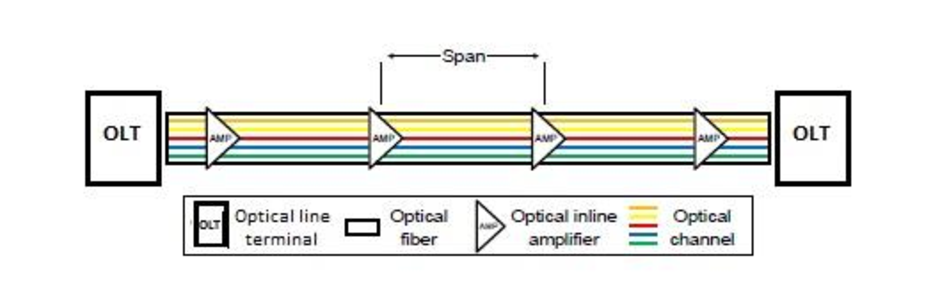
\includegraphics[width=\textwidth]{sdf/ILP/figures/link_design}
\caption{Design of a link.}
\label{link_design}
\end{figure}

\vspace{13pt}
Through the previous image, we can conclude that the link cost in monetary units (e.g. euros, or dollars), $C_L$, is calculated by the equation \ref{Capex_Link}

\begin{equation}
C_L = \sum_{i=1}^N \sum_{j=i+1}^N L_{ij} \bigg( 2 \gamma_0^{OLT} + 2 \gamma_1^{OLT} \tau W_{ij} + 2 N^R_{ij} c^R \bigg)
\label{Capex_Link}
\end{equation}

\noindent
where
\begin{itemize}
\item{$i$               $\rightarrow$   Index for start node of a physical link}
\item{$j$               $\rightarrow$   Index for end node of a physical link}
\item{$N$				$\rightarrow$	Total number of nodes, N $\in \mathbb{N}$}
\item{$L_{ij}$			$\rightarrow$	Binary variable indicating if link between the nodes $i$ and $j$ is used, $L_{ij} \in {0, 1}$}
\item{$\gamma_0^{OLT}$	$\rightarrow$	OLT cost in monetary units (e.g. euros, or dollars)}
\item{$\gamma_1^{OLT}$	$\rightarrow$	Transponder cost in monetary units (e.g. euros, or dollars)}
\item{$\tau$		    $\rightarrow$	Line bit-rate}
\item{$W_{ij}$          $\rightarrow$   Total number of optical channels in link $i$ $j$}
\item{$N^R_{ij}$    	$\rightarrow$	Number of optical amplifiers in link $i$ $j$}
\item{$c^R$				$\rightarrow$	Optical amplifiers cost in monetary units (e.g. euros, or dollars)}
\end{itemize}

\vspace{11pt}
The number of amplifiers for each link can be calculated by equation \ref{Capex_amplifiers}

\begin{equation}
N^R_{ij} = \sum_{i=1}^{N}\sum\limits_{j=i+1}^{N}\left(\left\lceil\frac{len_{ij}}{span}\right\rceil-1\right)
\label{Capex_amplifiers}
\end{equation}

\vspace{11pt}
\noindent
where the variable $len_{ij}$ is the length of link $ij$ in kilometers and the $span$ is the distance between amplifiers also in kilometers \cite{aulas}. For all cases this distance is always 100 km.\\

The next step is to take into account the cost of the nodes, but for this we must first know how a node is constituted. The nodes have an electrical part, $C_{EXC}$, and an optical part, $C_{OXC}$, so we can conclude that the cost of the nodes, $C_N$, is given by the sum of these two parts \cite{aulas} thus obtaining the equation \ref{Capex_Node}.

\begin{equation}
C_N = C_{EXC} + C_{OXC}
\label{Capex_Node}
\end{equation}

\vspace{11pt}
In relation to the electric part we can see the figure \ref{exc_design} where it shows its constitution.

\begin{figure}[h!]
\centering
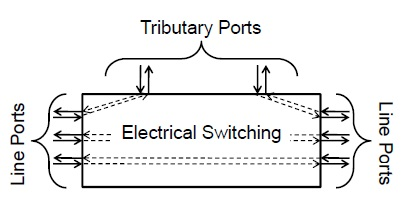
\includegraphics[width=8cm]{sdf/ILP/figures/exc_design}
\caption{Design of a electrical switching.}
\label{exc_design}
\end{figure}

Through this image, we can conclude in a simple way that the electric cost is the sum of the fixed cost of the electrical connection with the total cost of all the electric ports.\\
Therefore the electric cost in monetary units (e.g. euros, or dollars), $C_{EXC}$, is given by equation \ref{Capex_Node_EXC}\\

\begin{equation}
C_{EXC} = \sum_{n=1}^{N} N_{exc,n} \left( \gamma_{e0} + \sum_{c=-1}^B \gamma_{e1,c} P_{exc,c,n} \right)
\label{Capex_Node_EXC}
\end{equation}

\noindent
where
\begin{itemize}
\item{$N$				$\rightarrow$	Total number of nodes, N $\in \mathbb{N}$}
\item{$N_{exc,n}$		$\rightarrow$	Binary variable indicating if node $n$ is used, $N_{exc,n} \in {0, 1}$}
\item{$\gamma_{e0}$ 	$\rightarrow$	EXC cost in monetary units (e.g. euros, or dollars)}
\item{$\gamma_{e1,c}$	$\rightarrow$	EXC port cost in monetary units (e.g. euros, or dollars) with bit-rate $B$ and with a given transceiver reach}
\item{$P_{exc,c,n}$	    $\rightarrow$	Number of ports of the electrical switch}
\item{$B$           	$\rightarrow$	A natural number corresponding to the maximum index of short-reach ports, see table below}
\end{itemize}

\begin{table}[h!]
\centering
\begin{tabular}{|c|c|}
  \hline
  Index & Bit rate \\
 \hline\hline
  -1 & 100 Gbits/s line bit-rate (long-reach port) \\
  0 & 1.25 Gbits/s tributary bit-rate (short-reach port) \\
  1 & 2.5 Gbits/s tributary bit-rate (short-reach port) \\
  2 & 10 Gbits/s tributary bit-rate (short-reach port) \\
  3 & 40 Gbits/s tributary bit-rate (short-reach port) \\
  4 & 100 Gbits/s tributary bit-rate (short-reach port) \\
  \hline
\end{tabular}
\caption{Table with index and your corresponding bit rate}
\label{table_bitrate}
\end{table}

Now, in relation to the optical part through the figure \ref{oxc_design} we can see its constitution.\\

\begin{figure}[h!]
\centering
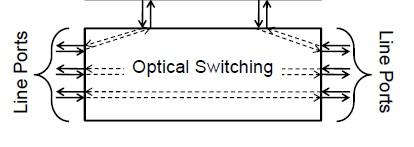
\includegraphics[width=8cm]{sdf/ILP/figures/oxc_design}
\caption{Design of a optical switching.}
\label{oxc_design}
\end{figure}

Through the previous image, we can conclude in a simple way that the optical cost is the sum of the fixed cost of the optical connection with the total cost of all the optical ports.
Therefore the optical cost in monetary units (e.g. euros, or dollars), $C_{OXC}$, is given by equation \ref{Capex_Node_OXC}

\begin{equation}
C_{OXC} = \sum_{n=1}^{N} N_{oxc,n} \bigg( \gamma_{o0} + \gamma_{o1} P_{oxc,n} \bigg)
\label{Capex_Node_OXC}
\end{equation}

\noindent
where
\begin{itemize}
\item{$N$				$\rightarrow$	Total number of nodes, N $\in \mathbb{N}$}
\item{$N_{oxc,n}$		$\rightarrow$	Binary variable indicating if node $n$ is used, $N_{oxc,n} \in {0, 1}$}
\item{$\gamma_{o0}$ 	$\rightarrow$	OXC cost in monetary units (e.g. euros, or dollars)}
\item{$\gamma_{o1}$ 	$\rightarrow$	OXC port cost in monetary units (e.g. euros, or dollars) }
\item{$P_{oxc,n}$	    $\rightarrow$	Number of ports of the optical switch}
\end{itemize}


\vspace{10pt}
We have to take into account that the calculated value for the variable $P_{exc,c,n}$ and $P_{oxc,n}$ will depend on the mode of transport used (opaque, transparent or translucent) but in next subsections will be explained how these values are calculated for each specific transport mode.\\

All transport modes require the routing of the demands. In this work we assume that the routing is performed by the ILP model instead of feeding it with candidate paths.\\
The flow conservation constraints ensures that, for each $(o,d)$ pair we route Z units of flow from node $o$ to node $d$. The flow conservation constraints are as follows \cite{teserui}:

\begin{equation}
\sum_{j=1\textbackslash \{o\}}^{N} f_{ij}^{od} = Z  \qquad \qquad \qquad \qquad \qquad \qquad \qquad \qquad \qquad
\forall(o,d) : o < d, \forall i: i = o
\label{ILPOpaque1_CAPEX}
\end{equation}
\noindent
Constraint \ref{ILPOpaque1_CAPEX} states that for each $(o,d)$ pair the node $o$ (being the source of the flow) sends Z units through one or more links $(i,j)$ such as $o=i$. The variable Z depends of the transport mode and survivability mechanism.

\begin{equation}
\sum_{j=1\textbackslash \{o\}}^{N} f_{ij}^{od} = \sum_{j=1\textbackslash \{d\}}^{N} f_{ji}^{od}   \qquad \qquad \qquad \qquad \qquad \qquad \qquad \qquad
\forall(o,d) : o < d, \forall i: i \neq o,d
\label{ILPOpaque2_CAPEX}
\end{equation}
\noindent
Constraint \ref{ILPOpaque2_CAPEX} ensures that the remaining nodes, being neither origin or destination of the flow, the amount of received flow have to be send.

\begin{equation}
\sum_{j=1\textbackslash \{d\}}^{N} f_{ji}^{od} = Z  \qquad \qquad \qquad \qquad \qquad \qquad \qquad \qquad \qquad \qquad
\forall(o,d) : o < d, \forall i: i = d
\label{ILPOpaque3_CAPEX}
\end{equation}
\noindent
Constraint \ref{ILPOpaque3_CAPEX} states that the destination node, $d$, has to receive those Z units of flow.\\

Finally, one aspect to be taken into account is the cost of the equipment used in the network. Through the table \ref{table_cost_ilp} we can see the cost in euros of the equipment.

\begin{table}[h!]
\centering
\begin{tabular}{|| c | c | c||}
 \hline
 Equipment & Symbol & Cost \\
 \hline\hline
 OLT without transponders & $\gamma_0^{OLT}$ & 15 000 \euro \\
 Transponder & $\gamma_1^{OLT}$ & 5 000 \euro/Gb \\
 Unidirectional Optical Amplifier & $c^R$ & 4 000 \euro \\
 EXC & $\gamma_{e0}$ & 10 000 \euro \\
 OXC & $\gamma_{o0}$ & 20 000 \euro \\
 EXC Port for line ports & $\gamma_{e1,-1}$ & 100 000 \euro /port\\
 EXC Port for ODU0 & $\gamma_{e1,0}$ & 10 \euro /port\\
 EXC Port for ODU1 & $\gamma_{e1,1}$ & 15 \euro /port\\
 EXC Port for ODU2 & $\gamma_{e1,2}$ & 30 \euro /port\\
 EXC Port for ODU3 & $\gamma_{e1,3}$ & 60 \euro /port\\
 EXC Port for ODU4 & $\gamma_{e1,4}$ & 100 \euro /port\\
 OXC Port & $\gamma_{o1}$ & 2 500 \euro /port \\
 \hline
\end{tabular}
\caption{Table of costs used to calculate CAPEX using ILP models \cite{aulas}.}
\label{table_cost_ilp}
\end{table}


%Subsection with the different transport mode
\clearpage

\subsection{Opaque without Survivability}\label{ILP_Opaque_Survivability}
\begin{tcolorbox}	
\begin{tabular}{p{2.75cm} p{0.2cm} p{10.5cm}} 	
\textbf{Student Name}  &:& Tiago Esteves    (October 03, 2017 - )\\
\textbf{Goal}          &:& Implement the ILP model for the opaque transport mode without survivability.
\end{tabular}
\end{tcolorbox}

\subsubsection{Model description}

First, for a better understanding of the functions and variables used in the ILP, a table \ref{description_opaque} will be created with all indexes, inputs and variables and with their respective description.\\

\begin{table}[h!]
\centering
\begin{tabular}{ |p{1cm}||p{13cm}|}
 \hline
 \multicolumn{2}{|c|}{Description of notation used in the objective function} \\
 \hline
 \hline
 $i$ & index for start node of a physical link \\
 $j$ & index for end node of a physical link \\
 $o$ & index for node that is origin of a demand \\
 $d$ & index for node that is destination of a demand \\
 $c$ & index for bit rate of the client signal \\
 $($ i,j $)$ & physical link between the nodes $i$ and $j$ \\
 $($ o,d $)$ & demand between the nodes $o$ and $d$ \\
 $C$ & set of the client signal \\
 $f_{ij}^{od}$ & binary variable indicating if link between the nodes $i$ and $j$ is used in the path between nodes $o$ and $d$ \\
 $L_{ij}$ & binary variable indicating if link between the nodes $i$ and $j$ is used \\
 $W_{ij}$ & number of optical channels between the nodes $i$ and $j$\\
 $B_c $ & client signals granularities $($1.25, 2.5, 10, 40, 100$)$ \\
 $D_{odc}$ & client demands with bit rate $c$ between nodes $o$ and $d$ \\
 $G_{ij}$ & network topology in form of adjacency matrix \\
 \hline
\end{tabular}
\caption{Table with description of variables}
\label{description_opaque}
\end{table}

Before carrying out the description of the objective function we must take into account the following particularity of this mode of transport:
\begin{itemize}
  \item $N_{OXC,n}$ = 0, \quad $\forall$ n
  \item $N_{EXC,n}$ = 1, \quad $\forall$ n that process traffic
\end{itemize}


\vspace{11pt}
The objective function of following the ILP is a minimization of the CAPEX through the equation \ref{Capex} where in this case for the cost of nodes we only have in consideration the electric cost \ref{Capex_Node_EXC} because of the particularity previously mentioned.
In this case the value of $P_{exc,c,n}$ is obtained by equation \ref{EXC_pexc1_opaque} for long-reach and by the equation \ref{EXC_pexc2_opaque} for short-reach.\\

\newpage
As previously mentioned, equation \ref{EXC_pexc1_opaque} refers to the number of long-reach ports, that is, the number of line ports of node n is calculated.

\begin{equation}
P_{exc,-1,n} = \sum_{j=1}^{N} w_{nj}
\label{EXC_pexc1_opaque}
\end{equation}

\begin{itemize}
\item{$P_{exc,-1,n}$	$\rightarrow$	Number of long-reach ports of the electrical switch, i.e. number of line ports}
\item{$w_{nj}$			$\rightarrow$	Number of optical channels between node $n$ and node $j$}
\end{itemize}

\vspace{11pt}
As previously mentioned, equation \ref{EXC_pexc2_opaque} refers to the number of sort-reach ports, that is, the number of tributary ports with bit-rate c in node n is calculated.

\begin{equation}
P_{exc,c,n} = \sum_{d=1}^{N} D_{nd,c}
\label{EXC_pexc2_opaque}
\end{equation}

\begin{itemize}
\item{$P_{exc,c,n}$	$\rightarrow$	Number of sort-reach ports of the electrical switch}
\item{$D_{nj,c}$	$\rightarrow$	client demands between nodes $n$ and $d$ with bit rate $c$}
\end{itemize}

\vspace{11pt}
In this case there is the following particularity:

\begin{itemize}
  \item When $n$=$j$ the value of client demands is always zero, i.e, $D_{nn,c}=0$
\end{itemize}


\vspace{17pt}
The objective function, to be minimized, is the expression \ref{ILPOpaque_CAPEX}.\\


$subject$ $to$
\begin{equation}
\sum_{j\textbackslash \{o\}} f_{ij}^{od} = 1  \qquad \qquad \qquad \qquad \qquad \qquad \qquad \qquad \qquad \qquad
\forall(o,d) : o < d, \forall i: i = o
\label{ILPOpaque1_Surv}
\end{equation}

This constraint are equal to the constraint \ref{ILPOpaque1_CAPEX} assuming that Z variable has the value of 1.

\begin{equation}
\sum_{j\textbackslash \{o\}} f_{ij}^{od} = \sum_{j\textbackslash \{d\}} f_{ji}^{od}   \qquad \qquad \qquad \qquad \qquad \qquad \qquad \qquad
\forall(o,d) : o < d, \forall i: i \neq o,d
\label{ILPOpaque2_Surv}
\end{equation}

This constraint are equal to the constraint \ref{ILPOpaque2_CAPEX}.

\begin{equation}
\sum_{j\textbackslash \{d\}} f_{ji}^{od} = 1  \qquad \qquad \qquad \qquad \qquad \qquad \qquad \qquad \qquad \qquad
\forall(o,d) : o < d, \forall i: i = d
\label{ILPOpaque3_Surv}
\end{equation}

This constraint are equal to the constraint \ref{ILPOpaque3_CAPEX} assuming that Z variable has the value of 1.

\begin{equation}
\sum_{(o,d):o<d} \left(f_{ij}^{od} + f_{ji}^{od}\right) + \sum_{c\in C} (B\left(c\right) D_{odc}\leq100 W_{ij} G_{ij} \qquad \qquad \qquad \qquad
\forall(i,j) : i < j
\label{ILPOpaque4_Surv}
\end{equation}

This restriction is considered grooming constraint, so it means the total client traffic flows can not be greater than the capacity of optical channels on all links.

\begin{equation}
W_{ij} \leq K_{ij} L_{ij} \qquad  \qquad \qquad \qquad \qquad \qquad \qquad \qquad \qquad \qquad \qquad \qquad \qquad \forall(i,j) : i < j
\label{ILPOpaque5_Surv}
\end{equation}

This restriction concerns the capacity of the optical channels which must be less or equal to the maximum number of optical channels. For any situation the maximum number of optical channels supported by each transmission system is 80, i.e., $K_{ij}$ = 80.

\begin{equation}
f_{ij}^{od} , f_{ji}^{od} \in \{0,1\}   \qquad \qquad \qquad \qquad \qquad \qquad \qquad \qquad \qquad
\forall(i,j) : i < j, \forall(o,d) : o < d
\label{ILPOpaque6_Surv}
\end{equation}

The number of flows per demand in this case can be zero if there are no traffic demands or one if considering traffic.

\begin{equation}
W_{ij} \in \mathbb{N}  \qquad \qquad \qquad \qquad \qquad \qquad \qquad \qquad \qquad \qquad \qquad \qquad \qquad
\forall(i,j) : i < j
\label{ILPOpaque7_Surv}
\end{equation}

The last constraint is just needed to ensure the number optical of channels is a positive integer values greater than zero.\\

 
\subsubsection{Result description}

To perform the calculations using the implementation of the models described in previous subsection it is necessary to use a mathematical software tool. For this we will use MATLAB which is ideal for dealing with linear programming problems and can call the LPsolve through an external interface.\\
We already have all the necessary to obtain the CAPEX value for the reference network \ref{Reference_Network_Topology}. As described in the subsection of network traffic \ref{Reference_Network_Traffic}, we have three values of network traffic (low, medium and high traffic) so we have to obtain three different CAPEX.
The value of the CAPEX of the network will be calculated based on the costs of the equipment present in the table \ref{table_cost_ilp}.
\newpage
\begin{table}[h!]
\centering
\begin{tabular}{|| c | c||}
 \hline
 Equipment & Cost \\
 \hline\hline
 OLT without transponders & 15000 \euro \\
 Transponder & 5000 \euro/Gb \\
 Unidirectional Optical Amplifier & 4000 \euro \\
 EXC & 10000 \euro \\
 OXC & 20000 \euro \\
 EXC Port & 1000 \euro /Gb/s\\
 OXC Port & 2500 \euro /porto \\
 \hline
\end{tabular}
\caption{Table with costs}
\label{table_cost_ilp}
\end{table}


\textbf{Low Traffic Scenario:}\\

In this scenario we have to take into account the traffic calculated in \ref{low_traffic_scenario}. In figure \ref{link_opaque_surv_ref_low} we can see the number of optical channels and the number of amplifiers for each link calculated through MatLab.\\
 
\begin{figure}[h!]
\centering
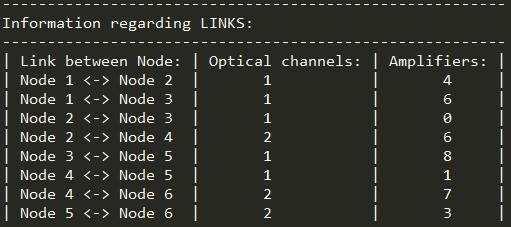
\includegraphics[width=10cm]{sdf/ilp/opaque_survivability/figures/link_opaque_surv_ref_low}
\caption{The ILP script used in the low scenario with the Link information.}
\label{link_opaque_surv_ref_low}
\end{figure}

In figure \ref{node_opaque_surv_ref_low}  we can see the number of transceivers, the number of line ports and the number of tributary ports for each node.\\

\begin{figure}[h!]
\centering
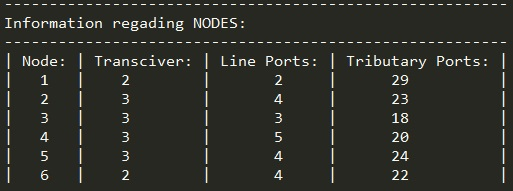
\includegraphics[width=10cm]{sdf/ilp/opaque_survivability/figures/node_opaque_surv_ref_low}
\caption{The ILP script used in the low scenario with the Node information.}
\label{node_opaque_surv_ref_low}
\end{figure}

Detailed description of each node:

Node 1:\\
- Needs 2 transceivers:\\
-- One to connect to Node 2;\\
-- One to connect to Node 3;\\
- Needs 2 line ports:\\
-- 1 line ports to connect to Node 2;\\
-- 1 line ports to connect to Node 3;\\
- Needs 29 tributary ports:\\
-- Where 13 is the ODU0;\\
-- Where 13 is the ODU1;\\
-- Where 3 is the ODU2;\\

Node 2:\\
- Needs 3 transceivers:\\
-- One to connect to Node 1;\\
-- One to connect to Node 3;\\
-- One to connect to Node 4;\\
- Needs 4 line ports:\\
-- 1 line ports to connect to Node 1;\\
-- 1 line ports to connect to Node 3;\\
-- 2 line ports to connect to Node 4;\\
- Needs 23 tributary ports:\\
-- Where 11 is the ODU0;\\
-- Where 7 is the ODU1;\\
-- Where 2 is the ODU2;\\
-- Where 2 is the ODU3;\\
-- Where 1 is the ODU4;\\

Node 3:\\
- Needs 3 transceivers:\\
-- One to connect to Node 1;\\
-- One to connect to Node 2;\\
-- One to connect to Node 5;\\
- Needs 3 line ports:\\
-- 1 line ports to connect to Node 1;\\
-- 1 line ports to connect to Node 2;\\
-- 1 line ports to connect to Node 5;\\
- Needs 18 tributary ports:\\
-- Where 7 is the ODU0;\\
-- Where 6 is the ODU1;\\
-- Where 3 is the ODU2;\\
-- Where 2 is the ODU3;\\

Node 4:\\
- Needs 3 transceivers:\\
-- One to connect to Node 2;\\
-- One to connect to Node 5;\\
-- One to connect to Node 6;\\
- Needs 5 line ports:\\
-- 2 line ports to connect to Node 2;\\
-- 1 line ports to connect to Node 5;\\
-- 2 line ports to connect to Node 6;\\
- Needs 20 tributary ports:\\
-- Where 7 is the ODU0;\\
-- Where 10 is the ODU1;\\
-- Where 3 is the ODU2;\\

Node 5:\\
- Needs 3 transceivers:\\
-- One to connect to Node 3;\\
-- One to connect to Node 4;\\
-- One to connect to Node 6;\\
- Needs 4 line ports:\\
-- 1 line ports to connect to Node 3;\\
-- 1 line ports to connect to Node 4;\\
-- 2 line ports to connect to Node 6;\\
- Needs 24 tributary ports:\\
-- Where 14 is the ODU0;\\
-- Where 4 is the ODU1;\\
-- Where 4 is the ODU2;\\
-- Where 1 is the ODU3;\\
-- Where 1 is the ODU4;\\

Node 6:\\
\quad - Needs 2 transceivers:\\
\quad \qquad - One to connect to Node 4;\\
\quad \qquad - One to connect to Node 5;\\
\quad - Needs 4 line ports:\\
\quad \qquad - 2 line ports to connect to Node 4;\\
\quad \qquad - 2 line ports to connect to Node 5;\\
\quad - Needs 22 tributary ports:\\
\quad \qquad - Where 8 is the ODU0;\\
\quad \qquad - Where 10 is the ODU1;\\
\quad \qquad - Where 1 is the ODU2;\\
\quad \qquad - Where 1 is the ODU3;\\
\quad \qquad - Where 2 is the ODU4;\\

Information regarding PATHS:\\

Path between Node1 <-> Node2:
\quad-Link(1,2)

Path between Node1 <-> Node3:
\quad-Link(1,3)

Path between Node1 <-> Node4:
\quad-Link(1,2) -Link(2,4)

Path between Node1 <-> Node5:
\quad-Link(1,3) -Link(3,5)

Path between Node1 <-> Node6:
\quad-Link(1,3) -Link(3,5) -Link(5,6)

Path between Node2 <-> Node3:
\quad-Link(2,3)

Path between Node2 <-> Node4:
\quad-Link(2,4)

Path between Node2 <-> Node5:
\quad-Link(2,3) -Link(3,5)

Path between Node2 <-> Node6:
\quad-Link(2,4) -Link(4,6)

Path between Node3 <-> Node4:
\quad-Link(3,2) -Link(2,4)

Path between Node3 <-> Node5:
\quad-Link(3,5)

Path between Node3 <-> Node6:
\quad-Link(3,5) -Link(5,6)

Path between Node4 <-> Node5:
\quad-Link(4,5)

Path between Node4 <-> Node6:
\quad-Link(4,6)

Path between Node5 <-> Node6:
\quad-Link(5,6)

\vspace{11pt}
Through the figure \ref{scriptopaque_surv_ref_low} we can see the result of CAPEX obtained with this ILP model.\\

\begin{figure}[h!]
\centering
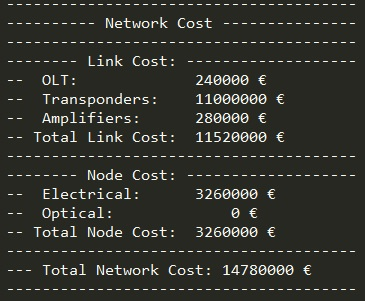
\includegraphics[width=10cm]{sdf/ilp/opaque_survivability/figures/script_opaque_surv_ref_low}
\caption{The ILP script used in the low scenario with the network cost.}
\label{scriptopaque_surv_ref_low}
\end{figure}

As we can see the cost of CAPEX for this scenario is \textbf{14 632 000 \euro}.\\


\textbf{Medium Traffic Scenario:}\\

In this scenario we have to take into account the traffic calculated in \ref{medium_traffic_scenario}. In table \ref{result_ILP2_reference} we can see the number of optical channels for each link calculated through MatLab and through the image \ref{scriptopaque_surv_ref_medium} we can see the results obtained with this ILP model.\\

\begin{table}[h!]
\centering
\begin{tabular}{|| c | c||}
 \hline
 Number of optical channels & Value \\
 \hline\hline
 in the link (1,2) & 5 \\
 in the link (1,3) & 3 \\
 in the link (2,3) & 5 \\
 in the link (2,4) & 8 \\
 in the link (3,5) & 5 \\
 in the link (4,5) & 3 \\
 in the link (4,6) & 3 \\
 in the link (5,6) & 3 \\
 \hline
\end{tabular}
\caption{Table with the number of optical channels for each link}
\label{result_ILP2_reference}
\end{table}


\begin{figure}[h!]
\centering
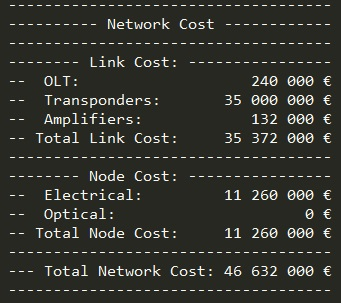
\includegraphics[width=10cm]{sdf/ilp/opaque_survivability/figures/script_opaque_surv_ref_medium}
\caption{The ILP script used in the medium scenario with the network cost.}
\label{scriptopaque_surv_ref_medium}
\end{figure}

As we can see the cost of CAPEX for this scenario is \textbf{46 632 000 \euro}.\\

\newpage
\textbf{High Traffic Scenario:}\\

In this scenario we have to take into account the traffic calculated in \ref{high_traffic_scenario}. In table \ref{result_ILP3_reference} we can see the number of optical channels for each link calculated through MatLab and through the image \ref{scriptopaque_surv_ref_high} we can see the results obtained with this ILP model.\\

\begin{table}[h!]
\centering
\begin{tabular}{|| c | c||}
 \hline
 Number of optical channels & Value \\
 \hline\hline
 in the link (1,2) & 4 \\
 in the link (1,3) & 4 \\
 in the link (2,3) & 4 \\
 in the link (2,4) & 19 \\
 in the link (3,5) & 9 \\
 in the link (4,5) & 5 \\
 in the link (4,6) & 16 \\
 in the link (5,6) & 14 \\
 \hline
\end{tabular}
\caption{Table with the number of optical channels for each link}
\label{result_ILP3_reference}
\end{table}


\begin{figure}[h!]
\centering
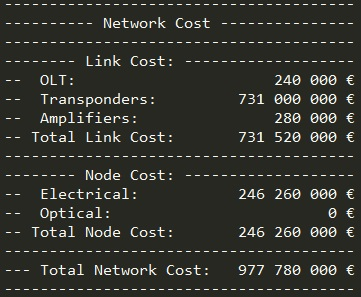
\includegraphics[width=10cm]{sdf/ilp/opaque_survivability/figures/script_opaque_surv_ref_high}
\caption{The ILP script used in the high scenario with the network cost.}
\label{scriptopaque_surv_ref_high}
\end{figure}

As we can see the cost of CAPEX for this scenario is \textbf{100 432 000 \euro}\\

\clearpage

\section{Opaque with 1+1 protection}\label{ILP_Opaque_Protection}

\subsection{Model description}

Once more, firstly in order to be able to apply the ILP model we have to take into account the physical and logical topologies allowed by this mode of transport and the type of survivability. Again based in section \ref{opaque} we can conclude that both topologies are the same and the following figures can be confirmed.\\

\begin{figure}[h!]
\centering
\includegraphics[width=10cm]{sdf/ilp/opaque_protection/figures/allowed_physical_topology}
\caption{Opaque with 1+1 protection: allowed physical topology. The allowed physical topology is defined by the duct and sites in the field. It is assumed that each duct supports up to 1 bidirectional transmission system and each site supports up to 1 node.}
\label{allowed_physical_protectionlow}
\end{figure}

\vspace{13pt}
\begin{figure}[h!]
\centering
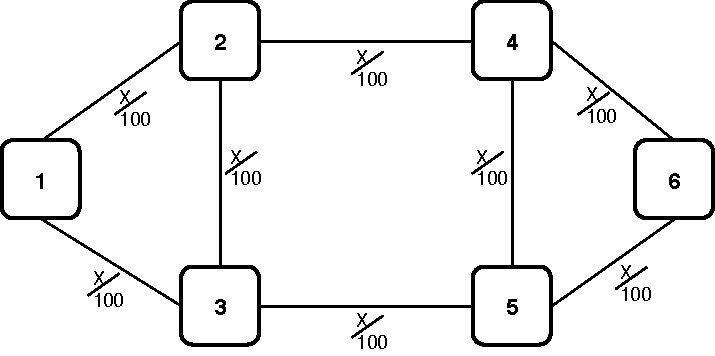
\includegraphics[width=10cm]{sdf/ilp/opaque_protection/figures/allowed_optical_topology}
\caption{Opaque with 1+1 protection: allowed optical topology. The allowed optical topology is defined by the transport mode. It is assumed that each transmission system supports up to 100 optical channels.}
\label{allowed_optical_protectionlow}
\end{figure}

Now taking this into account and based on the specific constraints of the opaque mode with 1+1 protection it is possible to define the ILP model \cite{tesevasco}.\\
\newpage
The objective function, to be minimized, is the expression \ref{Capex}, i.e.,

\begin{equation*}
  minimize \qquad \Big\{ \quad C_C \quad \Big\}
\end{equation*}

$subject$ $to$
\begin{equation}
\sum_{j=1\textbackslash \{o\}}^{N} fb_{ij}^{od} = 2  \qquad \qquad \qquad \qquad \qquad \qquad \qquad \qquad \qquad
\forall(o,d) : o < d, \forall i: i = o
\label{ILPOpaque1}
\end{equation}
\noindent
Constraint \ref{ILPOpaque1} is equal to the constraint \ref{ILPOpaque1_CAPEX} assuming that Z = 2.

\begin{equation}
\sum_{j=1\textbackslash \{o\}}^{N} fb_{ij}^{od} = \sum_{j=1\textbackslash \{d\}}^{N} f_{ji}^{od}   \qquad \qquad \qquad \qquad \qquad \qquad
\forall(o,d) : o < d, \forall i: i \neq o,d
\label{ILPOpaque2}
\end{equation}
\noindent
Constraint \ref{ILPOpaque2} is equal to the constraint \ref{ILPOpaque2_CAPEX}

\begin{equation}
\sum_{j=1\textbackslash \{d\}}^{N} fb_{ji}^{od} = 2  \qquad \qquad \qquad \qquad \qquad \qquad \qquad \qquad \qquad
\forall(o,d) : o < d, \forall i: i = d
\label{ILPOpaque3}
\end{equation}
\noindent
Constraint \ref{ILPOpaque3} is equal to the constraint \ref{ILPOpaque3_CAPEX} assuming that Z = 2.

\begin{equation}
\sum_{o=1}^{N} \sum_{d=o+1}^{N} \left(fb_{ij}^{od} + fb_{ji}^{od}\right) \sum_{c=1}^{C} (B\left(c\right) D_{odc})\leq \tau W_{ij} G_{ij} \qquad \qquad \qquad \qquad
\forall(i,j) : i < j
\label{ILPOpaque4}
\end{equation}
\noindent
The constraint \ref{ILPOpaque4} is considered the grooming constraint and is equal to the constraint \ref{ILPOpaque4_Surv} referred to in the case without survivability.

\begin{equation}
W_{ij} \leq K_{ij} L_{ij} \qquad \qquad \qquad \qquad \qquad \qquad \qquad \qquad \qquad \qquad \qquad \qquad \forall(i,j) : i < j
\label{ILPOpaque5}
\end{equation}
\noindent
Constraint \ref{ILPOpaque5} refers to the capacity of optical channels where they must be less or equal than the maximum number. For any situation, the maximum number of optical channels per transmission system is 100, that is, $K_{ij}$ = 100.

\begin{equation}
fb_{ij}^{od} , fb_{ji}^{od} , L_{ij} \in \{0,1\} \qquad \qquad \qquad \qquad \qquad \qquad \qquad
\forall(i,j) : i < j, \forall(o,d) : o < d
\label{ILPOpaque6}
\end{equation}
\noindent
The number of flows per demand in this case can be zero if there are no traffic demands or one if considering working or protection traffic, in relation to the use of the link, can be zero if it is not being used or one if is being used.
\newpage
\begin{equation}
W_{ij} \in \mathbb{N}  \qquad \qquad \qquad \qquad \qquad \qquad \qquad \qquad \qquad \qquad \qquad \qquad \qquad
\forall(i,j) : i < j\label{ILPOpaque7}
\end{equation}
\noindent
The last constraint is just needed to ensure the number of optical channels is a positive integer value.\\


\subsection{Result description}

As described in the subsection of network traffic \ref{Reference_Network_Traffic}, we have three values of network traffic so we have to obtain three different CAPEX.
The value of the CAPEX of the network will be calculated based on the costs of the equipment present in the table \ref{table_cost_ilp}.\\

\textbf{Low Traffic Scenario:}\\

In a first phase, we will show the resulting physical and optical topology. These topologies are based on the allowed topologies referred to in the model description and also taking into account the logical topology for all ODU's mentioned in the section \ref{low_scenario}.\\

\begin{figure}[h!]
\centering
\includegraphics[width=11cm]{sdf/ilp/opaque_protection/figures/physical_topology}
\caption{Opaque with 1+1 protection in low scenario: physical topology after dimensioning.}
\label{physical_protectionlow}
\end{figure}
\newpage
\begin{figure}[h!]
\centering
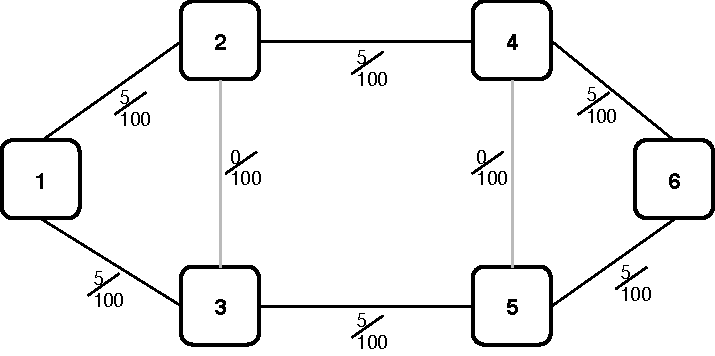
\includegraphics[width=11cm]{sdf/ilp/opaque_protection/figures/optical_topology_low}
\caption{Opaque with 1+1 protection in low scenario: optical topology after dimensioning.}
\label{optical_protectionlow}
\end{figure}

In table \ref{link_opaque_protec_ref_low} we can see the number of optical channels calculated using \ref{Capex_Link} and \ref{ILPOpaque_CAPEX} and the number of amplifiers for each link calculated using \ref{Capex_amplifiers}.

\begin{table}[h!]
\centering
\begin{tabular}{|| c | c | c ||}
 \hline
 \multicolumn{3}{|| c ||}{Information regarding links} \\
 \hline
 \hline
 Bidirectional Link & Optical Channels & Amplifiers\\
 \hline
 Node 1 <-> Node 2 & 2 & 4 \\
 Node 1 <-> Node 3 & 2 & 6 \\
 Node 2 <-> Node 3 & 3 & 0 \\
 Node 2 <-> Node 4 & 3 & 6 \\
 Node 3 <-> Node 5 & 3 & 8 \\
 Node 4 <-> Node 5 & 3 & 1 \\
 Node 4 <-> Node 6 & 3 & 7 \\
 Node 5 <-> Node 6 & 3 & 3 \\
 \hline
\end{tabular}
\caption{Table with information regarding links for opaque mode with 1+1 protection in low scenario.}
\label{link_opaque_protec_ref_low}
\end{table}

In table \ref{node_opaque_protec_ref_low} we can see the resulting nodal degree at the physical layer, calculated based on the number of connections that the node in question performs, the number of line ports calculated using \ref{EXC_pexc1_opaque} and the number of tributary ports calculated using \ref{EXC_pexc2_opaque} for each node.

\begin{table}[h!]
\centering
\begin{tabular}{|| c | c | c | c ||}
 \hline
 \multicolumn{4}{|| c ||}{Information regarding nodes} \\
 \hline
 \hline
 Node & Resulting Nodal Degree & Line Ports & Tributary Ports\\
 \hline
 1 & 2 & 4 & 29 \\
 2 & 3 & 8 & 23 \\
 3 & 3 & 8 & 18 \\
 4 & 3 & 9 & 20 \\
 5 & 3 & 9 & 24 \\
 6 & 2 & 6 & 22 \\
\hline
\end{tabular}
\caption{Table with information regarding nodes for opaque mode with 1+1 protection in low scenario.}
\label{node_opaque_protec_ref_low}
\end{table}
\newpage
Through the information obtained previously on the nodes we can now create tables with detailed information about each node. In each table mentioned below we can see how many ports are connected to a given node and its bit rate and how many ports are assigned to each different bit rate.

\begin{table}[h!]
\centering
\begin{tabular}{|| c | c | c ||}
 \hline
 \multicolumn{3}{|| c ||}{Detailed description of Node 1} \\
 \hline
 \hline
  & Number of tributary ports & Bit rate \\ \hline
\multirow{3}{*}{29 tributary ports} & 13 & ODU0 \\
 & 13 & ODU1 \\
 & 3 & ODU2 \\
 \hline
 \hline
  & Node<--Optical Channels-->Node & Bit rate \\
 \hline
 \multirow{2}{*}{4 line ports} & 1  <---- 2 ---->  2 & \multirow{2}{*}{100 Gbits/s} \\
 & 1  <---- 2 ---->  3 & \\
\hline
\end{tabular}
\caption{Opaque with 1+1 protection in low scenario: detailed description of node 1. The number of demands is distributed to the various destination nodes, this distribution can be observed in section \ref{low_scenario}.}
\end{table}

\begin{table}[h!]
\centering
\begin{tabular}{|| c | c | c ||}
 \hline
 \multicolumn{3}{|| c ||}{Detailed description of Node 2} \\
 \hline
 \hline
  & Number of total demands & Bit rate \\ \hline
\multirow{5}{*}{23 tributary ports} & 11 & ODU0 \\
 & 7 & ODU1 \\
 & 2 & ODU2 \\
 & 2 & ODU3 \\
 & 1 & ODU4 \\
 \hline
 \hline
  & Node<--Optical Channels-->Node & Bit rate \\ \hline
 \multirow{3}{*}{8 line ports} & 2  <---- 2 ---->  1 & \multirow{3}{*}{100 Gbits/s} \\
 & 2  <---- 3 ---->  3 & \\
 & 2  <---- 3 ---->  4 & \\
\hline
\end{tabular}
\caption{Opaque with 1+1 protection in low scenario: detailed description of node 2. The number of demands is distributed to the various destination nodes, this distribution can be observed in section \ref{low_scenario}.}
\end{table}

\begin{table}[h!]
\centering
\begin{tabular}{|| c | c | c ||}
 \hline
 \multicolumn{3}{|| c ||}{Detailed description of Node 3} \\
 \hline
 \hline
  & Number of total demands & Bit rate \\ \hline
\multirow{4}{*}{18 tributary ports} & 7 & ODU0 \\
 & 6 & ODU1\\
 & 3 & ODU2\\
 & 2 & ODU3\\
 \hline
 \hline
   & Node<--Optical Channels-->Node & Bit rate \\ \hline
 \multirow{3}{*}{8 line ports} & 3  <---- 2 ---->  1 & \multirow{3}{*}{100 Gbits/s}\\
 & 3  <---- 3 ---->  2 & \\
 & 3  <---- 3 ---->  5 & \\
\hline
\end{tabular}
\caption{Opaque with 1+1 protection in low scenario: detailed description of node 3. The number of demands is distributed to the various destination nodes, this distribution can be observed in section \ref{low_scenario}.}
\end{table}
\newpage
\begin{table}[h!]
\centering
\begin{tabular}{|| c | c | c ||}
 \hline
 \multicolumn{3}{|| c ||}{Detailed description of Node 4} \\
 \hline
 \hline
  & Number of total demands & Bit rate \\ \hline
\multirow{3}{*}{20 tributary ports} & 7 & ODU0 \\
 & 10 & ODU1 \\
 & 3 & ODU2 \\
 \hline
 \hline
   & Node<--Optical Channels-->Node & Bit rate \\ \hline
 \multirow{3}{*}{9 line ports} & 4  <---- 3 ---->  2 & \multirow{3}{*}{100 Gbits/s}\\
 & 4  <---- 3 ---->  5 & \\
 & 4  <---- 3 ---->  6 & \\
\hline
\end{tabular}
\caption{Opaque with 1+1 protection in low scenario: detailed description of node 4. The number of demands is distributed to the various destination nodes, this distribution can be observed in section \ref{low_scenario}.}
\end{table}

\begin{table}[h!]
\centering
\begin{tabular}{|| c | c | c ||}
 \hline
 \multicolumn{3}{|| c ||}{Detailed description of Node 5} \\
 \hline
 \hline
  & Number of total demands & Bit rate \\ \hline
\multirow{5}{*}{24 tributary ports} & 14 & ODU0 \\
 & 4 & ODU1 \\
 & 4 & ODU2 \\
 & 1 & ODU3 \\
 & 1 & ODU4 \\
 \hline
 \hline
   & Node<--Optical Channels-->Node & Bit rate \\ \hline
 \multirow{3}{*}{9 line ports} & 5  <---- 3 ---->  2 & \multirow{3}{*}{100 Gbits/s}\\
 & 5  <---- 3 ---->  4 & \\
 & 5  <---- 3 ---->  6 & \\
\hline
\end{tabular}
\caption{Opaque with 1+1 protection in low scenario: detailed description of node 5. The number of demands is distributed to the various destination nodes, this distribution can be observed in section \ref{low_scenario}.}
\end{table}

\begin{table}[h!]
\centering
\begin{tabular}{|| c | c | c ||}
 \hline
 \multicolumn{3}{|| c ||}{Detailed description of Node 6} \\
 \hline
 \hline
  & Number of total demands & Bit rate \\ \hline
\multirow{5}{*}{22 tributary ports} & 8 & ODU0 \\
 & 10 & ODU1 \\
 & 1 & ODU2 \\
 & 1 & ODU3 \\
 & 2 & ODU4 \\
 \hline
 \hline
   & Node<--Optical Channels-->Node & Bit rate \\ \hline
 \multirow{2}{*}{6 line ports} & 6  <---- 3 ---->  4 & \multirow{2}{*}{100 Gbits/s}\\
 & 6  <---- 3 ---->  5 & \\
\hline
\end{tabular}
\caption{Opaque with 1+1 protection in low scenario: detailed description of node 6. The number of demands is distributed to the various destination nodes, this distribution can be observed in section \ref{low_scenario}.}
\end{table}

\newpage
In the next table, we can see all the routing obtained for all nodes. These paths are bidirectional so the path from one node to another is the same path in the opposite direction. In the Links column we can see that there are two paths but it is not possible to distinguish them because we do not know which is protection and which is working.

\begin{table}[h!]
\centering
\begin{tabular}{|| c | c | c | c | c | c | c | c ||}
 \hline
 \multicolumn{8}{|| c ||}{Routing} \\
 \hline
 \hline
 o & d & Links & ODU0 & ODU1 & ODU2 & ODU3 & ODU4\\
 \hline
 \multirow{2}{*}{1} & \multirow{2}{*}{2} & \{(1,2)\} & \multirow{2}{*}{5} & \multirow{2}{*}{2} & \multirow{2}{*}{1} & \multirow{2}{*}{0} & \multirow{2}{*}{0} \\
 & & \{(1,3),(3,2)\} & & & & & \\ \hline
 \multirow{2}{*}{1} & \multirow{2}{*}{3} & \{(1,3)\} & \multirow{2}{*}{1} & \multirow{2}{*}{4} & \multirow{2}{*}{1} & \multirow{2}{*}{0} & \multirow{2}{*}{0}\\
 & & \{(1,2),(2,3)\} & & & & &\\ \hline
 \multirow{2}{*}{1} & \multirow{2}{*}{4} & \{(1,2),(2,4)\} & \multirow{2}{*}{3} & \multirow{2}{*}{2} & \multirow{2}{*}{1} & \multirow{2}{*}{0} & \multirow{2}{*}{0}\\
 & & \{(1,3),(3,5),(5,4)\} & & & & &\\ \hline
 \multirow{2}{*}{1} & \multirow{2}{*}{5} & \{(1,3),(3,5)\} & \multirow{2}{*}{1} & \multirow{2}{*}{0} & \multirow{2}{*}{0} & \multirow{2}{*}{0} & \multirow{2}{*}{0}\\
 & & \{(1,2),(2,4),(4,5)\} & & & & &\\ \hline
 \multirow{2}{*}{1} & \multirow{2}{*}{6} & \{(1,2),(2,4),(4,6)\} & \multirow{2}{*}{3} & \multirow{2}{*}{5} & \multirow{2}{*}{0} & \multirow{2}{*}{0} & \multirow{2}{*}{0}\\
 & & \{(1,3),(3,5),(5,6)\} & & & & &\\ \hline
 \multirow{2}{*}{2} & \multirow{2}{*}{3} & \{(2,3)\} & \multirow{2}{*}{0} & \multirow{2}{*}{0} & \multirow{2}{*}{0} & \multirow{2}{*}{1} & \multirow{2}{*}{0}\\
 & & \{(2,1),(1,3)\} & & & & &\\ \hline
 \multirow{2}{*}{2} & \multirow{2}{*}{4} & \{(2,4)\} & \multirow{2}{*}{1} & \multirow{2}{*}{3} & \multirow{2}{*}{0} & \multirow{2}{*}{0} & \multirow{2}{*}{0}\\
 & & \{(2,3),(3,5),(5,4)\} & & & & &\\ \hline
 \multirow{2}{*}{2} & \multirow{2}{*}{5} & \{(2,3),(3,5)\} & \multirow{2}{*}{5} & \multirow{2}{*}{1} & \multirow{2}{*}{1} & \multirow{2}{*}{0} & \multirow{2}{*}{0}\\
 & & \{(2,4),(4,5)\} & & & & &\\ \hline
 \multirow{2}{*}{2} & \multirow{2}{*}{6} & \{(2,4),(4,6)\} & \multirow{2}{*}{0} & \multirow{2}{*}{1} & \multirow{2}{*}{0} & \multirow{2}{*}{1} & \multirow{2}{*}{1}\\
 & & \{(2,3),(3,5),(5,6)\} & & & & &\\ \hline
 \multirow{2}{*}{3} & \multirow{2}{*}{4} & \{(3,2),(2,4)\} & \multirow{2}{*}{1} & \multirow{2}{*}{1} & \multirow{2}{*}{1} & \multirow{2}{*}{0} & \multirow{2}{*}{0}\\
 & & \{(3,5),(5,4)\} & & & & &\\ \hline
 \multirow{2}{*}{3} & \multirow{2}{*}{5} & \{(3,5)\} & \multirow{2}{*}{4} & \multirow{2}{*}{1} & \multirow{2}{*}{1} & \multirow{2}{*}{1} & \multirow{2}{*}{0}\\
 & & \{(3,1),(1,2),(2,4),(4,5)\} & & & & &\\ \hline
 \multirow{2}{*}{3} & \multirow{2}{*}{6} & \{(3,5),(5,6)\} & \multirow{2}{*}{1} & \multirow{2}{*}{0} & \multirow{2}{*}{0} & \multirow{2}{*}{0} & \multirow{2}{*}{0}\\
 & & \{(3,2),(2,4),(4,6)\} & & & & &\\ \hline
 \multirow{2}{*}{4} & \multirow{2}{*}{5} & \{(4,5)\} & \multirow{2}{*}{1} & \multirow{2}{*}{1} & \multirow{2}{*}{1} & \multirow{2}{*}{0} & \multirow{2}{*}{0}\\
 & & \{(4,6),(6,5)\} & & & & &\\ \hline
 \multirow{2}{*}{4} & \multirow{2}{*}{6} & \{(4,6)\} & \multirow{2}{*}{1} & \multirow{2}{*}{3} & \multirow{2}{*}{0} & \multirow{2}{*}{0} & \multirow{2}{*}{0}\\
 & & \{(4,5),(5,6)\} & & & & &\\ \hline
 \multirow{2}{*}{5} & \multirow{2}{*}{6} & \{(5,6)\} & \multirow{2}{*}{3} & \multirow{2}{*}{1} & \multirow{2}{*}{1} & \multirow{2}{*}{0} & \multirow{2}{*}{1}\\
 & & \{(5,4),(4,6)\} & & & & &\\
 \hline
\end{tabular}
\caption{Opaque with 1+1 protection in low scenario: description of routing. We are assuming that between a pair of nodes all demands follow the same route.}
\label{path_opaque_protec_ref_low}
\end{table}

Finally, in next page, through table \ref{scriptopaque_protec_ref_low} we can see the CAPEX result for this model. This value is obtained using equation \ref{ILPOpaque_CAPEX} and all of the constraints mentioned above.\\
\newpage
\begin{table}[h!]
\centering
\begin{tabular}{|| c | c | c | c | c | c | c ||}
 \hline
 \multicolumn{7}{|| c ||}{CAPEX of the Network} \\
 \hline
 \hline
 \multicolumn{3}{|| c |}{ } & Quantity & Unit Price & Cost & Total \\
 \hline
 \multirow{3}{*}{\makecell{Link \\ Cost}} & \multicolumn{2}{ c |}{OLTs} & 16 & 15 000 \euro & 240 000 \euro & \multirow{3}{*}{22 520 000 \euro} \\ \cline{2-6}
 & \multicolumn{2}{ c |}{100 Gbits/s Transceivers} & 44 & 5 000 \euro/Gbit/s & 22 000 000 \euro & \\ \cline{2-6}
 & \multicolumn{2}{ c |}{Amplifiers} & 70 & 4 000 \euro & 280 000 \euro & \\
 \hline
 \multirow{9}{*}{\makecell{Node \\ Cost}} & \multirow{7}{*}{Electrical} & EXCs & 6 & 10 000 \euro & 60 000 \euro & \multirow{9}{*}{4 462 590 \euro} \\ \cline{3-6}
 & & ODU0 Ports & 60 & 10 \euro/port & 600 \euro & \\ \cline{3-6}
 & & ODU1 Ports & 50 & 15 \euro/port & 750 \euro & \\ \cline{3-6}
 & & ODU2 Ports & 16 & 30 \euro/port & 480 \euro & \\ \cline{3-6}
 & & ODU3 Ports & 6 & 60 \euro/port & 360 \euro & \\ \cline{3-6}
 & & ODU4 Ports & 4 & 100 \euro/port & 400 \euro & \\ \cline{3-6}
 & & Line Ports & 44 & 100 000 \euro/port & 4 400 000 \euro & \\ \cline{2-6}
 & \multirow{2}{*}{Optical} & OXCs & 0 & 20 000 \euro & 0 \euro & \\ \cline{3-6}
 & & Ports & 0 & 2 500 \euro/porto & 0 \euro & \\
 \hline
 \multicolumn{6}{|| c |}{Total Network Cost} & 26 982 590 \euro \\
\hline
\end{tabular}
\caption{Opaque with 1+1 protection in low scenario: detailed description of CAPEX for this scenario.}
\label{scriptopaque_protec_ref_low}
\end{table}


\textbf{Medium Traffic Scenario:}\\

In a first phase, we will show the resulting physical and optical topology. These topologies are based on the allowed topologies referred to in the model description and also taking into account the logical topology for all ODU's mentioned in the section \ref{medium_traffic_scenario}.\\

\begin{figure}[h!]
\centering
\includegraphics[width=11cm]{sdf/ilp/opaque_protection/figures/physical_topology}
\caption{Opaque with 1+1 protection in medium scenario: physical topology after dimensioning.}
\label{physical_protectionmedium}
\end{figure}
\newpage
\begin{figure}[h!]
\centering
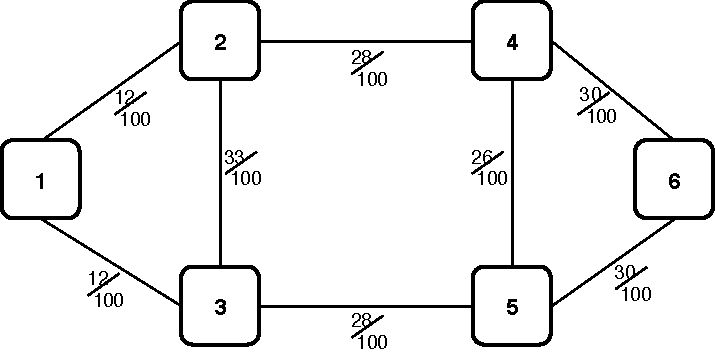
\includegraphics[width=11cm]{sdf/ilp/opaque_protection/figures/optical_topology_medium}
\caption{Opaque with 1+1 protection in medium scenario: optical topology after dimensioning.}
\label{optical_protectionmedium}
\end{figure}

Through table \ref{link_opaque_protec_ref_medium} we can see the number of optical channels calculated using \ref{Capex_Link} and \ref{ILPOpaque_CAPEX} and the number of amplifiers for each link calculated using \ref{Capex_amplifiers}.

\begin{table}[h!]
\centering
\begin{tabular}{|| c | c | c ||}
 \hline
 \multicolumn{3}{|| c ||}{Information regarding links} \\
 \hline
 \hline
 Bidirectional Link & Optical Channels & Amplifiers\\
 \hline
 Node 1 <-> Node 2 & 12 & 4 \\
 Node 1 <-> Node 3 & 12 & 6 \\
 Node 2 <-> Node 3 & 33 & 0 \\
 Node 2 <-> Node 4 & 28 & 6 \\
 Node 3 <-> Node 5 & 28 & 8 \\
 Node 4 <-> Node 5 & 26 & 1 \\
 Node 4 <-> Node 6 & 30 & 7 \\
 Node 5 <-> Node 6 & 30 & 3 \\
 \hline
\end{tabular}
\caption{Table with information regarding links for opaque mode with 1+1 protection in medium scenario.}
\label{link_opaque_protec_ref_medium}
\end{table}

We can see the resulting nodal degree at the physical layer, calculated based on the number of connections that the node in question performs, the number of line ports calculated using \ref{EXC_pexc1_opaque} and the number of tributary ports calculated using \ref{EXC_pexc2_opaque} for each node in table \ref{node_opaque_protec_ref_medium}.

\begin{table}[h!]
\centering
\begin{tabular}{|| c | c | c | c ||}
 \hline
 \multicolumn{4}{|| c ||}{Information regarding nodes} \\
 \hline
 \hline
 Node & Connections & Line Ports & Tributary Ports\\
 \hline
 1 & 2 & 24 & 290 \\
 2 & 3 & 73 & 230 \\
 3 & 3 & 73 & 180 \\
 4 & 3 & 84 & 200 \\
 5 & 3 & 84 & 240 \\
 6 & 2 & 60 & 220 \\
\hline
\end{tabular}
\caption{Table with information regarding nodes for opaque mode with 1+1 protection in medium scenario.}
\label{node_opaque_protec_ref_medium}
\end{table}

\newpage
Once more through the information obtained previously on the nodes we can now create tables with detailed information about each node. In each table mentioned below we can see how many ports are connected to a given node and its bit rate and how many ports are assigned to each different bit rate.

\begin{table}[h!]
\centering
\begin{tabular}{|| c | c | c ||}
 \hline
 \multicolumn{3}{|| c ||}{Detailed description of Node 1} \\
 \hline
 \hline
  & Number of total demands & bit rate \\ \hline
\multirow{3}{*}{290 tributary ports} & 130 & ODU0 \\
 & 130 & ODU1 \\
 & 30 & ODU2 \\
 \hline
 \hline
  & Node <-- Optical Channels --> Node & bit rate \\ \hline
\multirow{2}{*}{24 line ports} & 1  <---- 12 ---->  2 & \multirow{2}{*}{100 Gbtis/s} \\
 & 1  <---- 12 ---->  3 & \\
\hline
\end{tabular}
\caption{Opaque with 1+1 protection in medium scenario: detailed description of node 1. The number of demands is distributed to the various destination nodes, this distribution can be observed in section \ref{medium_traffic_scenario}.}
\end{table}

\begin{table}[h!]
\centering
\begin{tabular}{|| c | c | c ||}
 \hline
 \multicolumn{3}{|| c ||}{Detailed description of Node 2} \\
 \hline
 \hline
  & Number of total demands & bit rate \\ \hline
\multirow{5}{*}{230 tributary ports} & 110 & ODU0 \\
 & 70 & ODU1 \\
 & 20 & ODU2 \\
 & 20 & ODU3 \\
 & 10 & ODU4 \\
 \hline
 \hline
  & Node <-- Optical Channels --> Node & bit rate \\ \hline
 \multirow{3}{*}{73 line ports} & 2  <---- 12 ---->  1 & \multirow{3}{*}{100 Gbtis/s}\\
 & 2  <---- 33 ---->  3 & \\
 & 2  <---- 28 ---->  4 & \\
\hline
\end{tabular}
\caption{Opaque with 1+1 protection in medium scenario: detailed description of node 2. The number of demands is distributed to the various destination nodes, this distribution can be observed in section \ref{medium_traffic_scenario}.}
\end{table}

\begin{table}[h!]
\centering
\begin{tabular}{|| c | c | c ||}
 \hline
 \multicolumn{3}{|| c ||}{Detailed description of Node 3} \\
 \hline
 \hline
  & Number of total demands & bit rate \\ \hline
\multirow{4}{*}{180 tributary ports} & 70 & ODU0 \\
 & 60 & ODU1\\
 & 30 & ODU2\\
 & 20 & ODU3\\
  & Node <-- Optical Channels --> Node & bit rate \\ \hline
 \multirow{3}{*}{73 line ports} & 3  <---- 12 ---->  1 & \multirow{3}{*}{100 Gbtis/s}\\
 & 3  <---- 33 ---->  2 & \\
 & 3  <---- 28 ---->  5 & \\
\hline
\end{tabular}
\caption{Opaque with 1+1 protection in medium scenario: detailed description of node 3. The number of demands is distributed to the various destination nodes, this distribution can be observed in section \ref{medium_traffic_scenario}.}
\end{table}

\newpage
\begin{table}[h!]
\centering
\begin{tabular}{|| c | c | c ||}
 \hline
 \multicolumn{3}{|| c ||}{Detailed description of Node 4} \\
 \hline
 \hline
  & Number of total demands & bit rate \\ \hline
\multirow{3}{*}{200 tributary ports} & 70 & ODU0 \\
 & 100 & ODU1 \\
 & 30 & ODU2 \\
  & Node <-- Optical Channels --> Node & bit rate \\ \hline
\multirow{3}{*}{84 line ports} & 4  <---- 28 ---->  2 & \multirow{3}{*}{100 Gbtis/s}\\
 & 4  <---- 26 ---->  5 & \\
 & 4  <---- 30 ---->  6 & \\
\hline
\end{tabular}
\caption{Opaque with 1+1 protection in medium scenario: detailed description of node 4. The number of demands is distributed to the various destination nodes, this distribution can be observed in section \ref{medium_traffic_scenario}.}
\end{table}

\begin{table}[h!]
\centering
\begin{tabular}{|| c | c | c ||}
 \hline
 \multicolumn{3}{|| c ||}{Detailed description of Node 5} \\
 \hline
 \hline
  & Number of total demands & bit rate \\ \hline
\multirow{5}{*}{240 tributary ports} & 140 & ODU0 \\
 & 40 & ODU1 \\
 & 40 & ODU2 \\
 & 10 & ODU3 \\
 & 10 & ODU4 \\
  & Node <-- Optical Channels --> Node & bit rate \\ \hline
 \multirow{3}{*}{84 line ports} & 5  <---- 28 ---->  3 & \multirow{3}{*}{100 Gbtis/s} \\
 & 5  <---- 26 ---->  4 & \\
 & 5  <---- 30 ---->  6 & \\
\hline
\end{tabular}
\caption{Opaque with 1+1 protection in medium scenario: detailed description of node 5. The number of demands is distributed to the various destination nodes, this distribution can be observed in section \ref{medium_traffic_scenario}.}
\end{table}

\begin{table}[h!]
\centering
\begin{tabular}{|| c | c | c ||}
 \hline
 \multicolumn{3}{|| c ||}{Detailed description of Node 6} \\
 \hline
 \hline
  & Number of total demands & bit rate \\ \hline
\multirow{5}{*}{220 tributary ports} & 80 & ODU0 \\
 & 100 & ODU1 \\
 & 10 & ODU2 \\
 & 10 & ODU3 \\
 & 20 & ODU4 \\
  & Node <-- Optical Channels --> Node & bit rate \\ \hline
 \multirow{2}{*}{60 line ports} & 6  <---- 30 ---->  4 & \multirow{2}{*}{100 Gbtis/s} \\
 & 6  <---- 30 ---->  5 & \\
\hline
\end{tabular}
\caption{Opaque with 1+1 protection in medium scenario: detailed description of node 6. The number of demands is distributed to the various destination nodes, this distribution can be observed in section \ref{medium_traffic_scenario}.}
\end{table}

\newpage
Now let's focus on the routing information. These paths are bidirectional so the path from one node to another is the same path in the opposite direction. In table \ref{path_opaque_protec_ref_medium} we can see all the routing obtained for all nodes. In the Links column we can see that there are two paths but it is not possible to distinguish them because we do not know which is protection and which is working.\\

\begin{table}[h!]
\centering
\begin{tabular}{|| c | c | c | c | c | c | c | c ||}
 \hline
 \multicolumn{8}{|| c ||}{Routing} \\
 \hline
 \hline
 o & d & Links & ODU0 & ODU1 & ODU2 & ODU3 & ODU4\\
 \hline
 \multirow{2}{*}{1} & \multirow{2}{*}{2} & \{(1,2)\} & \multirow{2}{*}{50} & \multirow{2}{*}{20} & \multirow{2}{*}{10} & \multirow{2}{*}{0} & \multirow{2}{*}{0} \\
 & & \{(1,3),(3,2)\} & & & & & \\ \hline
 \multirow{2}{*}{1} & \multirow{2}{*}{3} & \{(1,3)\} & \multirow{2}{*}{10} & \multirow{2}{*}{40} & \multirow{2}{*}{10} & \multirow{2}{*}{0} & \multirow{2}{*}{0}\\
 & & \{(1,2),(2,3)\} & & & & &\\ \hline
 \multirow{2}{*}{1} & \multirow{2}{*}{4} & \{(1,2),(2,4)\} & \multirow{2}{*}{30} & \multirow{2}{*}{20} & \multirow{2}{*}{10} & \multirow{2}{*}{0} & \multirow{2}{*}{0}\\
 & & \{(1,3),(3,5),(5,4)\} & & & & &\\ \hline
 \multirow{2}{*}{1} & \multirow{2}{*}{5} & \{(1,3),(3,5)\} & \multirow{2}{*}{10} & \multirow{2}{*}{0} & \multirow{2}{*}{0} & \multirow{2}{*}{0} & \multirow{2}{*}{0}\\
 & & \{(1,2),(2,4),(4,5)\} & & & & &\\ \hline
 \multirow{2}{*}{1} & \multirow{2}{*}{6} & \{(1,2),(2,4),(4,6)\} & \multirow{2}{*}{30} & \multirow{2}{*}{50} & \multirow{2}{*}{0} & \multirow{2}{*}{0} & \multirow{2}{*}{0}\\
 & & \{(1,3),(3,5),(5,6)\} & & & & &\\ \hline
 \multirow{2}{*}{2} & \multirow{2}{*}{3} & \{(2,3)\} & \multirow{2}{*}{0} & \multirow{2}{*}{0} & \multirow{2}{*}{0} & \multirow{2}{*}{10} & \multirow{2}{*}{0}\\
 & & \{(2,1),(1,3)\} & & & & &\\ \hline
 \multirow{2}{*}{2} & \multirow{2}{*}{4} & \{(2,4)\} & \multirow{2}{*}{10} & \multirow{2}{*}{30} & \multirow{2}{*}{0} & \multirow{2}{*}{0} & \multirow{2}{*}{0}\\
 & & \{(2,3),(3,5),(5,4)\} & & & & &\\ \hline
 \multirow{2}{*}{2} & \multirow{2}{*}{5} & \{(2,4),(4,5)\} & \multirow{2}{*}{50} & \multirow{2}{*}{10} & \multirow{2}{*}{10} & \multirow{2}{*}{0} & \multirow{2}{*}{0}\\
 & & \{(2,3),(3,5)\} & & & & &\\ \hline
 \multirow{2}{*}{2} & \multirow{2}{*}{6} & \{(2,4),(4,6)\} & \multirow{2}{*}{0} & \multirow{2}{*}{10} & \multirow{2}{*}{0} & \multirow{2}{*}{10} & \multirow{2}{*}{10}\\
 & & \{(2,3),(3,5),(5,6)\} & & & & &\\ \hline
 \multirow{2}{*}{3} & \multirow{2}{*}{4} & \{(3,2),(2,4)\} & \multirow{2}{*}{10} & \multirow{2}{*}{10} & \multirow{2}{*}{10} & \multirow{2}{*}{0} & \multirow{2}{*}{0}\\
 & & \{(3,5),(5,4)\} & & & & &\\ \hline
 \multirow{2}{*}{3} & \multirow{2}{*}{5} & \{(3,5)\} & \multirow{2}{*}{40} & \multirow{2}{*}{10} & \multirow{2}{*}{10} & \multirow{2}{*}{10} & \multirow{2}{*}{0}\\
 & & \{(3,2),(2,4),(4,5)\} & & & & &\\ \hline
 \multirow{2}{*}{3} & \multirow{2}{*}{6} & \{(3,5),(5,6)\} & \multirow{2}{*}{10} & \multirow{2}{*}{0} & \multirow{2}{*}{0} & \multirow{2}{*}{0} & \multirow{2}{*}{0}\\
 & & \{(3,2),(2,4),(4,6)\} & & & & &\\ \hline
 \multirow{2}{*}{4} & \multirow{2}{*}{5} & \{(4,5)\} & \multirow{2}{*}{10} & \multirow{2}{*}{10} & \multirow{2}{*}{10} & \multirow{2}{*}{0} & \multirow{2}{*}{0}\\
 & & \{(4,6),(6,5)\} & & & & &\\ \hline
 \multirow{2}{*}{4} & \multirow{2}{*}{6} & \{(4,6)\} & \multirow{2}{*}{10} & \multirow{2}{*}{30} & \multirow{2}{*}{0} & \multirow{2}{*}{0} & \multirow{2}{*}{0}\\
 & & \{(4,5),(5,6)\} & & & & &\\ \hline
 \multirow{2}{*}{5} & \multirow{2}{*}{6} & \{(5,6)\} & \multirow{2}{*}{30} & \multirow{2}{*}{10} & \multirow{2}{*}{10} & \multirow{2}{*}{0} & \multirow{2}{*}{10}\\
 & & \{(5,4),(4,6)\} & & & & &\\
 \hline
\end{tabular}
\caption{Opaque with 1+1 protection in medium scenario: table with description of routing. We are assuming that between a pair of nodes all demands follow the same route.}
\label{path_opaque_protec_ref_medium}
\end{table}

Once more in next page, through table \ref{scriptopaque_protec_ref_medium} we can see the CAPEX result for this model. This value is obtained using equation \ref{ILPOpaque_CAPEX} and all of the constraints mentioned above.\\
\newpage
\begin{table}[h!]
\centering
\begin{tabular}{||c|c|c|c|c|c|c||}
 \hline
 \multicolumn{7}{||c||}{CAPEX of the Network} \\
 \hline
 \hline
 \multicolumn{3}{||c|}{}& Quantity & Unit Price & Cost & Total \\
 \hline
 \multirow{3}{*}{\makecell{Link \\ Cost}} & \multicolumn{2}{c|}{OLTs}&16&15 000 \euro&240 000 \euro&\multirow{3}{*}{199 520 000 \euro}\\ \cline{2-6}
 & \multicolumn{2}{c|}{100 Gbits/s Transceivers}&398&5 000 \euro/Gbit/s&199 000 000 \euro&\\ \cline{2-6}
 & \multicolumn{2}{c|}{Amplifiers}&70&4 000 \euro&280 000 \euro&\\
 \hline
 \multirow{9}{*}{\makecell{Node \\ Cost}}&\multirow{7}{*}{Electrical}&EXCs & 6 & 10 000 \euro & 60 000 \euro & \multirow{9}{*}{39 885 900 \euro} \\ \cline{3-6}
 & &ODU0 Ports& 600 & 10 \euro/port & 6 000 \euro & \\ \cline{3-6}
 & &ODU1 Ports& 500 & 15 \euro/port & 7 500 \euro & \\ \cline{3-6}
 & &ODU2 Ports& 160 & 30 \euro/port & 4 800 \euro & \\ \cline{3-6}
 & &ODU3 Ports& 60 & 60 \euro/port & 3 600 \euro & \\ \cline{3-6}
 & &ODU4 Ports& 40 & 100 \euro/port & 4 000 \euro & \\ \cline{3-6}
 & &Line Ports& 398 &100 000 \euro/port&39 800 000 \euro& \\ \cline{2-6}
 & \multirow{2}{*}{Optical} & OXCs & 0 & 20 000 \euro & 0 \euro & \\ \cline{3-6}
 & & Ports & 0 & 2 500 \euro/porto & 0 \euro & \\
 \hline
 \multicolumn{6}{|| c |}{Total Network Cost} & 239 405 900 \euro \\
\hline
\end{tabular}
\caption{Opaque with 1+1 protection in medium scenario: table with detailed description of CAPEX for this scenario.}
\label{scriptopaque_protec_ref_medium}
\end{table}


\textbf{High Traffic Scenario:}\\

In a first phase, we will show the resulting physical and optical topology. These topologies are based on the allowed topologies referred to in the model description and also taking into account the logical topology for all ODU's mentioned in the section \ref{high_traffic_scenario}.\\

\begin{figure}[h!]
\centering
\includegraphics[width=11cm]{sdf/ilp/opaque_protection/figures/physical_topology}
\caption{Opaque with 1+1 protection in high scenario: physical topology after dimensioning.}
\label{physical_protectionhigh}
\end{figure}

\newpage
\begin{figure}[h!]
\centering
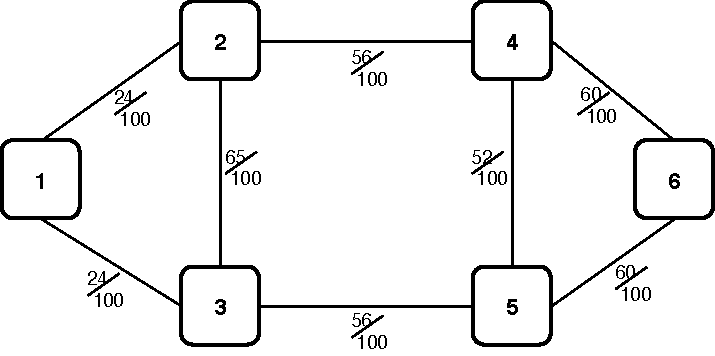
\includegraphics[width=11cm]{sdf/ilp/opaque_protection/figures/optical_topology_high}
\caption{Opaque with 1+1 protection in high scenario: optical topology after dimensioning.}
\label{optical_protectionhigh}
\end{figure}

In table \ref{link_opaque_protec_ref_high} we can see the number of optical channels calculated using \ref{Capex_Link} and \ref{Capex} and the number of amplifiers for each link calculated using \ref{amplifiers}.

\begin{table}[h!]
\centering
\begin{tabular}{|| c | c | c ||}
 \hline
 \multicolumn{3}{|| c ||}{Information regarding links} \\
 \hline
 \hline
 Bidirectional Link & Optical Channels & Amplifiers\\
 \hline
 Node 1 <-> Node 2 & 24 & 4 \\
 Node 1 <-> Node 3 & 24 & 6 \\
 Node 2 <-> Node 3 & 65 & 0 \\
 Node 2 <-> Node 4 & 56 & 6 \\
 Node 3 <-> Node 5 & 56 & 8 \\
 Node 4 <-> Node 5 & 52 & 1 \\
 Node 4 <-> Node 6 & 60 & 7 \\
 Node 5 <-> Node 6 & 60 & 3 \\
 \hline
\end{tabular}
\caption{Table with information regarding links for opaque mode with 1+1 protection in high scenario.}
\label{link_opaque_protec_ref_high}
\end{table}

In table \ref{node_opaque_protec_ref_high} we can see the resulting nodal degree at the physical layer, calculated based on the number of connections that the node in question performs, the number of line ports calculated using \ref{EXC_pexc1_opaque} and the number of tributary ports calculated using \ref{EXC_pexc2_opaque} for each node.

\begin{table}[h!]
\centering
\begin{tabular}{|| c | c | c | c ||}
 \hline
 \multicolumn{4}{|| c ||}{Information regarding nodes} \\
 \hline
 \hline
 Node & Resulting Nodal Degree & Line Ports & Tributary Ports\\
 \hline
 1 & 2 & 48 & 580 \\
 2 & 3 & 145 & 460 \\
 3 & 3 & 145 & 360 \\
 4 & 3 & 168 & 400 \\
 5 & 3 & 168 & 480 \\
 6 & 2 & 120 & 440 \\
\hline
\end{tabular}
\caption{Table with information regarding nodes for opaque mode with 1+1 protection in high scenario.}
\label{node_opaque_protec_ref_high}
\end{table}

\newpage
Once again, through the information obtained previously on the nodes we can now create tables with detailed information about each node. In each table mentioned below we can see how many ports are connected to a given node and its bit rate and how many ports are assigned to each different bit rate.

\begin{table}[h!]
\centering
\begin{tabular}{|| c | c | c ||}
 \hline
 \multicolumn{3}{|| c ||}{Detailed description of Node 1} \\
 \hline
 \hline
  & Number of total demands & bit rate \\ \hline
\multirow{3}{*}{580 tributary ports} & 260 & ODU0 \\
 & 260 & ODU1 \\
 & 60 & ODU2 \\
  & Node <-- Optical Channels --> Node & bit rate \\ \hline
\multirow{2}{*}{48 line ports} & 1  <---- 24 ---->  2 & \multirow{2}{*}{100 Gbtis/s} \\
 & 1  <---- 24 ---->  3 & \\
\hline
\end{tabular}
\caption{Opaque with 1+1 protection in high scenario: detailed description of node 1. The number of demands is distributed to the various destination nodes, this distribution can be observed in section \ref{high_traffic_scenario}.}
\end{table}

\begin{table}[h!]
\centering
\begin{tabular}{|| c | c | c ||}
 \hline
 \multicolumn{3}{|| c ||}{Detailed description of Node 2} \\
 \hline
 \hline
  & Number of total demands & bit rate \\ \hline
\multirow{5}{*}{460 tributary ports} & 220 & ODU0 \\
 & 140 & ODU1 \\
 & 40 & ODU2 \\
 & 40 & ODU3 \\
 & 20 & ODU4 \\
  & Node <-- Optical Channels --> Node & bit rate \\ \hline
 \multirow{3}{*}{145 line ports} & 2  <---- 24 ---->  1 & \multirow{3}{*}{100 Gbtis/s}\\
 & 2  <---- 65 ---->  3 & \\
 & 2  <---- 56 ---->  4 & \\
\hline
\end{tabular}
\caption{Opaque with 1+1 protection in high scenario: detailed description of node 2. The number of demands is distributed to the various destination nodes, this distribution can be observed in section \ref{high_traffic_scenario}.}
\end{table}

\begin{table}[h!]
\centering
\begin{tabular}{|| c | c | c ||}
 \hline
 \multicolumn{3}{|| c ||}{Detailed description of Node 3} \\
 \hline
 \hline
  & Number of total demands & bit rate \\ \hline
\multirow{4}{*}{360 tributary ports} & 140 & ODU0 \\
 & 120 & ODU1\\
 & 60 & ODU2\\
 & 40 & ODU3\\
  & Node <-- Optical Channels --> Node & bit rate \\ \hline
 \multirow{3}{*}{145 line ports} & 3  <---- 24 ---->  1 & \multirow{3}{*}{100 Gbtis/s}\\
 & 3  <---- 65 ---->  2 & \\
 & 3  <---- 56 ---->  5 & \\
\hline
\end{tabular}
\caption{Opaque with 1+1 protection in high scenario: detailed description of node 3. The number of demands is distributed to the various destination nodes, this distribution can be observed in section \ref{high_traffic_scenario}.}
\end{table}

\newpage
\begin{table}[h!]
\centering
\begin{tabular}{|| c | c | c ||}
 \hline
 \multicolumn{3}{|| c ||}{Detailed description of Node 4} \\
 \hline
 \hline
  & Number of total demands & bit rate \\ \hline
\multirow{3}{*}{400 tributary ports} & 140 & ODU0 \\
 & 200 & ODU1 \\
 & 60 & ODU2 \\
  & Node <-- Optical Channels --> Node & bit rate \\ \hline
\multirow{3}{*}{168 line ports} & 4  <---- 56 ---->  2 & \multirow{3}{*}{100 Gbtis/s}\\
 & 4  <---- 52 ---->  5 & \\
 & 4  <---- 60 ---->  6 & \\
\hline
\end{tabular}
\caption{Opaque with 1+1 protection in high scenario: detailed description of node 4. The number of demands is distributed to the various destination nodes, this distribution can be observed in section \ref{high_traffic_scenario}.}
\end{table}

\begin{table}[h!]
\centering
\begin{tabular}{|| c | c | c ||}
 \hline
 \multicolumn{3}{|| c ||}{Detailed description of Node 5} \\
 \hline
 \hline
  & Number of total demands & bit rate \\ \hline
\multirow{5}{*}{480 tributary ports} & 280 & ODU0 \\
 & 80 & ODU1 \\
 & 80 & ODU2 \\
 & 20 & ODU3 \\
 & 20 & ODU4 \\
  & Node <-- Optical Channels --> Node & bit rate \\ \hline
 \multirow{3}{*}{168 line ports} & 5  <---- 56 ---->  3 & \multirow{3}{*}{100 Gbtis/s} \\
 & 5  <---- 52 ---->  4 & \\
 & 5  <---- 60 ---->  6 & \\
\hline
\end{tabular}
\caption{Opaque with 1+1 protection in high scenario: detailed description of node 5. The number of demands is distributed to the various destination nodes, this distribution can be observed in section \ref{high_traffic_scenario}.}
\end{table}

\begin{table}[h!]
\centering
\begin{tabular}{|| c | c | c ||}
 \hline
 \multicolumn{3}{|| c ||}{Detailed description of Node 6} \\
 \hline
 \hline
  & Number of total demands & bit rate \\ \hline
\multirow{5}{*}{440 tributary ports} & 160 & ODU0 \\
 & 200 & ODU1 \\
 & 20 & ODU2 \\
 & 20 & ODU3 \\
 & 40 & ODU4 \\
  & Node <-- Optical Channels --> Node & bit rate \\ \hline
 \multirow{2}{*}{120 line ports} & 6  <---- 60 ---->  4 & \multirow{2}{*}{100 Gbtis/s} \\
 & 6  <---- 60 ---->  5 & \\
\hline
\end{tabular}
\caption{Opaque with 1+1 protection in high scenario: detailed description of node 6. The number of demands is distributed to the various destination nodes, this distribution can be observed in section \ref{high_traffic_scenario}.}
\end{table}

\newpage
Now through the table \ref{path_opaque_protec_ref_high} we can see all the routing obtained for all nodes. These paths are bidirectional so the path from one node to another is the same path in the opposite direction. In the Links column we can see that there are two paths but it is not possible to distinguish them because we do not know which is protection and which is working.

\begin{table}[h!]
\centering
\begin{tabular}{|| c | c | c | c | c | c | c | c ||}
 \hline
 \multicolumn{8}{|| c ||}{Routing} \\
 \hline
 \hline
 o & d & Links & ODU0 & ODU1 & ODU2 & ODU3 & ODU4\\
 \hline
 \multirow{2}{*}{1} & \multirow{2}{*}{2} & \{(1,2)\} & \multirow{2}{*}{100} & \multirow{2}{*}{40} & \multirow{2}{*}{20} & \multirow{2}{*}{0} & \multirow{2}{*}{0} \\
 & & \{(1,3),(3,2)\} & & & & & \\ \hline
 \multirow{2}{*}{1} & \multirow{2}{*}{3} & \{(1,3)\} & \multirow{2}{*}{20} & \multirow{2}{*}{80} & \multirow{2}{*}{20} & \multirow{2}{*}{0} & \multirow{2}{*}{0}\\
 & & \{(1,2),(2,3)\} & & & & &\\ \hline
 \multirow{2}{*}{1} & \multirow{2}{*}{4} & \{(1,2),(2,4)\} & \multirow{2}{*}{60} & \multirow{2}{*}{40} & \multirow{2}{*}{20} & \multirow{2}{*}{0} & \multirow{2}{*}{0}\\
 & & \{(1,3),(3,5),(5,4)\} & & & & &\\ \hline
 \multirow{2}{*}{1} & \multirow{2}{*}{5} & \{(1,3),(3,5)\} & \multirow{2}{*}{20} & \multirow{2}{*}{0} & \multirow{2}{*}{0} & \multirow{2}{*}{0} & \multirow{2}{*}{0}\\
 & & \{(1,2),(2,4),(4,5)\} & & & & &\\ \hline
 \multirow{2}{*}{1} & \multirow{2}{*}{6} & \{(1,2),(2,4),(4,6)\} & \multirow{2}{*}{60} & \multirow{2}{*}{100} & \multirow{2}{*}{0} & \multirow{2}{*}{0} & \multirow{2}{*}{0}\\
 & & \{(1,3),(3,5),(5,6)\} & & & & &\\ \hline
 \multirow{2}{*}{2} & \multirow{2}{*}{3} & \{(2,3)\} & \multirow{2}{*}{0} & \multirow{2}{*}{0} & \multirow{2}{*}{0} & \multirow{2}{*}{20} & \multirow{2}{*}{0}\\
 & & \{(2,1),(1,3)\} & & & & &\\ \hline
 \multirow{2}{*}{2} & \multirow{2}{*}{4} & \{(2,4)\} & \multirow{2}{*}{20} & \multirow{2}{*}{60} & \multirow{2}{*}{0} & \multirow{2}{*}{0} & \multirow{2}{*}{0}\\
 & & \{(2,3),(3,5),(5,4)\} & & & & &\\ \hline
 \multirow{2}{*}{2} & \multirow{2}{*}{5} & \{(2,4),(4,5)\} & \multirow{2}{*}{100} & \multirow{2}{*}{20} & \multirow{2}{*}{20} & \multirow{2}{*}{0} & \multirow{2}{*}{0}\\
 & & \{(2,3),(3,5)\} & & & & &\\ \hline
 \multirow{2}{*}{2} & \multirow{2}{*}{6} & \{(2,4),(4,6)\} & \multirow{2}{*}{0} & \multirow{2}{*}{20} & \multirow{2}{*}{0} & \multirow{2}{*}{20} & \multirow{2}{*}{20}\\
 & & \{(2,3),(3,5),(5,6)\} & & & & &\\ \hline
 \multirow{2}{*}{3} & \multirow{2}{*}{4} & \{(3,2),(2,4)\} & \multirow{2}{*}{20} & \multirow{2}{*}{20} & \multirow{2}{*}{20} & \multirow{2}{*}{0} & \multirow{2}{*}{0}\\
 & & \{(3,5),(5,4)\} & & & & &\\ \hline
 \multirow{2}{*}{3} & \multirow{2}{*}{5} & \{(3,5)\} & \multirow{2}{*}{80} & \multirow{2}{*}{20} & \multirow{2}{*}{20} & \multirow{2}{*}{20} & \multirow{2}{*}{0}\\
 & & \{(3,2),(2,4),(4,5)\} & & & & &\\ \hline
 \multirow{2}{*}{3} & \multirow{2}{*}{6} & \{(3,5),(5,6)\} & \multirow{2}{*}{20} & \multirow{2}{*}{0} & \multirow{2}{*}{0} & \multirow{2}{*}{0} & \multirow{2}{*}{0}\\
 & & \{(3,2),(2,4),(4,6)\} & & & & &\\ \hline
 \multirow{2}{*}{4} & \multirow{2}{*}{5} & \{(4,5)\} & \multirow{2}{*}{20} & \multirow{2}{*}{20} & \multirow{2}{*}{20} & \multirow{2}{*}{0} & \multirow{2}{*}{0}\\
 & & \{(4,6),(6,5)\} & & & & &\\ \hline
 \multirow{2}{*}{4} & \multirow{2}{*}{6} & \{(4,6)\} & \multirow{2}{*}{20} & \multirow{2}{*}{60} & \multirow{2}{*}{0} & \multirow{2}{*}{0} & \multirow{2}{*}{0}\\
 & & \{(4,5),(5,6)\} & & & & &\\ \hline
 \multirow{2}{*}{5} & \multirow{2}{*}{6} & \{(5,6)\} & \multirow{2}{*}{60} & \multirow{2}{*}{20} & \multirow{2}{*}{20} & \multirow{2}{*}{0} & \multirow{2}{*}{20}\\
 & & \{(5,4),(4,6)\} & & & & &\\
 \hline
\end{tabular}
\caption{Opaque with 1+1 protection in high scenario: description of routing. We are assuming that between a pair of nodes all demands follow the same route.}
\label{path_opaque_protec_ref_high}
\end{table}

Finally in next page, through table \ref{scriptopaque_protec_ref_high} we can see the CAPEX result for this model. This value is obtained using equation \ref{ILPOpaque_CAPEX} and all of the constraints mentioned above.\\
\newpage
\begin{table}[h!]
\centering
\begin{tabular}{||c|c|c|c|c|c|c||}
 \hline
 \multicolumn{7}{||c||}{CAPEX of the Network} \\
 \hline
 \hline
 \multicolumn{3}{||c|}{} & Quantity & Unit Price & Cost & Total \\
 \hline
 \multirow{3}{*}{\makecell{Link \\ Cost}} &\multicolumn{2}{c|}{OLTs}&16&15 000 \euro&240 000 \euro&\multirow{3}{*}{397 520 000 \euro}\\ \cline{2-6}
 & \multicolumn{2}{c|}{100 Gbits/s Transceivers}&794&5 000 \euro/Gbit/s&397 000 000 \euro&\\ \cline{2-6}
 & \multicolumn{2}{c|}{Amplifiers} & 70 & 4 000 \euro & 280 000 \euro & \\
 \hline
 \multirow{9}{*}{\makecell{Node \\ Cost}} &\multirow{7}{*}{Electrical}&EXCs&6& 10 000 \euro & 60 000 \euro & \multirow{9}{*}{79 511 800 \euro} \\ \cline{3-6}
 & &ODU0 Ports&1 200& 10 \euro/port & 12 000 \euro & \\ \cline{3-6}
 & &ODU1 Ports&1 000& 15 \euro/port & 15 000 \euro & \\ \cline{3-6}
 & &ODU2 Ports& 320 & 30 \euro/port & 9 600 \euro & \\ \cline{3-6}
 & &ODU3 Ports& 120 & 60 \euro/port & 7 200 \euro & \\ \cline{3-6}
 & &ODU4 Ports& 80 & 100 \euro/port & 8 000 \euro & \\ \cline{3-6}
 & &Line Ports& 794 &100 000 \euro/port&79 400 000 \euro&\\ \cline{2-6}
 & \multirow{2}{*}{Optical} & OXCs & 0 & 20 000 \euro & 0 \euro & \\ \cline{3-6}
 & & Ports & 0 & 2 500 \euro/porto & 0 \euro & \\
 \hline
 \multicolumn{6}{||c|}{Total Network Cost} &477 031 800 \euro \\
\hline
\end{tabular}
\caption{Opaque with 1+1 protection in high scenario: detailed description of CAPEX for this scenario.}
\label{scriptopaque_protec_ref_high}
\end{table}

\subsection{Conclusions}

Once we have obtained the results for all the scenarios we will now draw some conclusions about these results. For a better analysis of the results will be created the table \ref{table_comparative_opaque_protec} with the number of line ports, tributary ports and transceivers because they are important values for the cost of CAPEX, the cost of links, the cost of nodes and finally the cost of CAPEX.\\

\begin{table}[h!]
\centering
\begin{tabular}{| c | c | c | c |}
 \hline
  & Low Traffic & Medium Traffic  & High Traffic \\
 \hline\hline
 CAPEX without survivability&11 266 590 \euro&90 605 900 \euro&178 231 800 \euro\\ \hline
 CAPEX/Gbit/s without survivability&22 533 \euro/Gbit/s&18 121 \euro/Gbit/s&17 823 \euro/Gbit/s\\ \hline
 Traffic (Gbit/s) & 500 & 5 000 & 10 000 \\ \hline
 Bidirectional Links used & 8 & 8 & 8 \\ \hline
 Number of Line ports & 44 & 398 & 794 \\ \hline
 Number of Tributary ports & 136 & 1 360 & 2 720 \\ \hline
 Number of Transceivers & 44 & 398 & 794 \\ \hline
 Link Cost & 22 520 000 \euro & 199 520 000 \euro & 397 520 000 \euro \\ \hline
 Node Cost & 4 462 590 \euro & 39 885 900 \euro & 79 511 800 \euro \\ \hline
 CAPEX & \textbf{26 982 590 \euro} & \textbf{239 405 900 \euro} & \textbf{477 031 800 \euro} \\ \hline
 CAPEX/Gbit/s & \textbf{53 965 \euro/Gbit/s} & \textbf{47 881 \euro/Gbit/s} & \textbf{47 703 \euro/Gbit/s}\\
 \hline
\end{tabular}
\caption{Opaque with 1+1 protection: Table with the various CAPEX values obtained in the different traffic scenarios.}
\label{table_comparative_opaque_protec}
\end{table}

Looking at the previous table we can make some comparisons between the several scenarios:

\begin{itemize}
  \item All scenarios uses all available links. This is because in this case regardless of traffic we always need two possible paths.
  \item Comparing the low traffic with the others we can see that despite having an increase of factor ten (medium traffic) and factor twenty (high traffic), the same increase does not occur in the final cost (it is lower). This happens because the number of the transceivers is lower than expected which leads by carrying the traffic with less network components and, consequently, the network CAPEX is lower.
  \item Comparing the medium traffic with the high traffic we can see that the increase of the factor is double and in the final cost this factor is very close but still inferior. This happens because the number of the transceivers is also lower but very close to the expected.
  \item Comparing the CAPEX cost per bit we can see that in the low traffic the cost is higher than the medium and high traffic, which in these two cases the value is very similar. This happens because the lower the traffic, the higher CAPEX/bit will be. We can see that in medium and high traffic the results tend to be one closer value.
  \item Comparing this cost with the without survivability cost we can conclude that protection is significantly more expensive. As can be seen in the table this increase is more than double as with 1+1 protection we have a cost more than twice than the cost without survivability.
\end{itemize}

\clearpage

\subsection{Transparent without Survivability}\label{ILP_Transp_Survivability}
\begin{tcolorbox}	
\begin{tabular}{p{2.75cm} p{0.2cm} p{10.5cm}} 	
\textbf{Student Name}  &:& Tiago Esteves    (October 03, 2017 - )\\
\textbf{Goal}          &:& Implement the ILP model for the transparent transport mode without survivability.
\end{tabular}
\end{tcolorbox}

\subsubsection{Model description}

First, for a better understanding of the functions and variables used in the ILP, a table \ref{description_transp} will be created with all indexes, inputs and variables and with their respective description.

\begin{table}[h!]
\centering
\begin{tabular}{ |p{1cm}||p{13cm}|}
 \hline
 \multicolumn{2}{|c|}{Description of notation used in the objective function} \\
 \hline
 \hline
 $i$ & index for start node of a physical link \\
 $j$ & index for end node of a physical link \\
 $o$ & index for node that is origin of a demand \\
 $d$ & index for node that is destination of a demand \\
 $c$ & index for bit rate of the client signal \\
 $($ i,j $)$ & physical link between the nodes $i$ and $j$ \\
 $($ o,d $)$ & demand between the nodes $o$ and $d$ \\
 $C$ & set of the client signal \\
 $f_{ij}^{od}$ & the number of 100 Gbit/s optical channels between the nodes $o$ and $d$ that uses link ($i$,$j$) \\
 $fp_{ij}^{od}$ & the number of 100 Gbit/s optical channels (with protection) between the nodes $o$ and $d$ that uses link ($i$,$j$) \\
 $L_{ij}$ & binary variable indicating if link between the nodes $i$ and $j$ is used \\
 $\lambda_{od}$ & the number of 100 Gbit/s optical channels between the nodes $o$ and $d$ \\
 $D_{odc}$ & client demands between nodes $o$ and $d$ with bit rate $c$ \\
 $G$ & Network topology in form of adjacency matrix \\
 \hline
\end{tabular}
\caption{Table with description of variables}
\label{description_transp}
\end{table}

Before carrying out the description of the objective function we must take into account the following particularity of this mode of transport:
\begin{itemize}
  \item $N_{OXC,n}$ = 1, \quad $\forall$ n that process traffic
  \item $N_{EXC,n}$ = 1, \quad $\forall$ n that process traffic
\end{itemize}

\vspace{7pt}
The objective function of following the ILP is a minimization of the CAPEX through the equation \ref{Capex} where in this case for the cost of nodes we have in consideration electric \ref{Capex_Node_EXC} and optical cost \ref{Capex_Node_OXC}. In this case the value of $P_{exc,c,n}$ is obtained by equation \ref{EXC_pexc1_transparent} for short-reach and by the equation \ref{EXC_pexc2_transparent} for long-reach and the value of $P_{oxc,n}$ is obtained by equation \ref{OXC_poxc_transparent}.\\

The equation \ref{EXC_pexc1_transparent} refers to the number of sort-reach ports of the electrical switch with bit-rate $c$ in node $n$, $P_{exc,c,n}$, i.e. the number of tributary ports with bit-rate $c$ in node $n$ which can be calculated as

\begin{equation}
P_{exc,c,n} = \sum_{d=1}^{N} D_{nd,c}
\label{EXC_pexc1_transparent}
\end{equation}

\vspace{11pt}
\noindent
where $D_{nd,c}$ are the client demands between nodes $n$ and $d$ with bit rate $c$.\\

In this case there is the following particularity:
\begin{itemize}
  \item When $n$=$d$ the value of client demands is always zero, i.e, $D_{nn,c}=0$
\end{itemize}

\vspace{11pt}
As previously mentioned, the equation \ref{EXC_pexc2_transparent} refers to the number of long-reach ports of the electrical switch with bit-rate -1 in node n, $P_{exc,-1,n}$, i.e. the number of add ports of node n which can be calculated as

\begin{equation}
P_{exc,-1,n} = \sum_{j=1}^{N} \lambda_{nj}
\label{EXC_pexc2_transparent}
\end{equation}

\vspace{11pt}
\noindent
where $\lambda_{nj}$ is the number of optical channels between node $n$ and node $j$.\\

The equation \ref{OXC_poxc_transparent} refers to the number of ports in optical switch in node n, $P_{oxc,n}$, i.e. the number of line ports and the number of adding ports of node n which can be calculated as

\begin{equation}
P_{oxc,n} = \sum_{j=1}^{N} f_{nj}^{od} + \sum_{j=1}^{N} \lambda_{nj}
\label{OXC_poxc_transparent}
\end{equation}

\vspace{11pt}
\noindent
where $f_{nj}^{od}$ refers to the number of line ports for all demand pairs (od) and $\lambda_{nj}$ refers to the number of add ports.\\

The objective function, to be minimized, is the expression \ref{ILPOpaque_CAPEX}, i.e.,
\begin{equation*}
  minimize \qquad \Big\{ \quad C_C \quad \Big\}
\end{equation*}

$subject$ $to$
\begin{equation}
\sum_{c\in C} B\left(c\right) D_{odc} \leq \tau \lambda_{od} \qquad \qquad \qquad \qquad \qquad \qquad \qquad \qquad \qquad \qquad
\forall(o,d) : o < d
\label{ILPTransp0_surv}
\end{equation}

This restriction is considered grooming constraint and for this model the grooming can be done before routing since the traffic is aggregated just for demands between the same nodes, thus not depending on the routes. The variable  $\tau$ is always 100 Gbits/s.

\begin{equation}
\sum_{j\textbackslash \{o\}} f_{ij}^{od} = \lambda_{od}  \qquad \qquad \qquad \qquad \qquad \qquad \qquad \qquad \qquad
\forall(o,d) : o < d, \forall i: i = o
\label{ILPTransp1_surv}
\end{equation}

This constraint are equal to the constraint \ref{ILPOpaque1_CAPEX} assuming that Z variable has the value of number of optical channels between this demand for all bidirectional links.

\begin{equation}
\sum_{j\textbackslash \{o\}} f_{ij}^{od} = \sum_{j\textbackslash \{d\}} f_{ji}^{od} \qquad \qquad \qquad \qquad \qquad \qquad \qquad \qquad
\forall(o,d) : o < d, \forall i: i \neq o,d
\label{ILPTransp2_surv}
\end{equation}

This constraint are equal to the constraint \ref{ILPOpaque2_CAPEX}.

\begin{equation}
\sum_{j\textbackslash \{d\}} f_{ji}^{od} = \lambda_{od}  \qquad \qquad \qquad \qquad \qquad \qquad \qquad \qquad \qquad
\forall(o,d) : o < d, \forall i: i = d
\label{ILPTransp3_surv}
\end{equation}

This constraint are equal to the constraint \ref{ILPOpaque3_CAPEX} assuming that Z variable has the value of number of optical channels between this demand for all bidirectional links.

\begin{equation}
\sum_{o=1} \sum_{d=o+1} \left(f_{ij}^{od} + f_{ji}^{od}\right) \leq K_{ij} G_{ij} L_{ij} \qquad \qquad \qquad \qquad \qquad \qquad \qquad
\forall(i,j) : i < j
\label{ILPTransp4_surv}
\end{equation}

This restriction answers capacity constraint problem. Then, total flows must be less or equal to the capacity of network links. For any situation the maximum number of optical channels supported by each transmission system is 100, i.e., $K_{ij}$ = 100.

\begin{equation}
f_{ij}^{od} , f_{ji}^{od} , \lambda_{od} \in \mathbb{N}   \qquad \qquad \qquad \qquad \qquad \qquad \qquad \qquad
\forall(i,j) : i < j, \forall(o,d) : o < d
\label{ILPTransp5_surv}
\end{equation}

Last constraint define the total number of flows and the number of optical channels must be a counting number.\\


\subsubsection{Result description}

To perform the calculations using the implementation of the models described previously it is necessary to use a mathematical software tool. For this we will use MATLAB which is ideal for dealing with linear programming problems and can call the LPsolve through an external interface.\\
We already have all the necessary to obtain the CAPEX value for the reference network \ref{Reference_Network_Topology}. As described in the subsection of network traffic \ref{Reference_Network_Traffic}, we have three values of network traffic (low, medium and high traffic) so we have to obtain three different CAPEX.
The value of the CAPEX of the network will be calculated based on the costs of the equipment present in the table \ref{table_cost_ilp}.

\newpage
\textbf{Low Traffic Scenario:}\\

In this scenario we have to take into account the traffic calculated in \ref{low_scenario}. In a first phase we will show the various existing topologies of the network. The first are the allowed topologies, physical and optical topology, the second are the logical topology for all ODUs and finally the resulting physical and optical topology.\\

\begin{figure}[h!]
\centering
\includegraphics[width=12cm]{sdf/ilp/transparent_survivability/figures/allowed_physical_topology}
\caption{Allowed physical topology. The allowed physical topology is defined by the duct and sites in the field. It is assumed that each duct supports up to 1 bidirectional transmission system and each site supports up to 1 node.}
\label{allowed2_physical_low}
\end{figure}

\vspace{11pt}
\begin{figure}[h!]
\centering
\includegraphics[width=12cm]{sdf/ilp/transparent_survivability/figures/allowed_optical_topology}
\caption{Allowed optical topology. The allowed optical topology is defined by the transport mode (transparent transport mode in this case). It is assumed that each connections between demands supports up to 100 lightpaths.}
\label{allowed2_optical_low}
\end{figure}

\newpage
\begin{figure}[h!]
\centering
\includegraphics[width=12cm]{sdf/ilp/transparent_survivability/figures/logical_topology_ODU0_low}
\caption{ODU0 logical topology defined by the ODU0 traffic matrix.}
\label{logical2_ODU0_low}
\end{figure}

\begin{figure}[h!]
\centering
\includegraphics[width=12cm]{sdf/ilp/transparent_survivability/figures/logical_topology_ODU1_low}
\caption{ODU1 logical topology defined by the ODU1 traffic matrix.}
\label{logical2_ODU1_low}
\end{figure}

\begin{figure}[h!]
\centering
\includegraphics[width=12cm]{sdf/ilp/transparent_survivability/figures/logical_topology_ODU2_low}
\caption{ODU2 logical topology defined by the ODU2 traffic matrix.}
\label{logical2_ODU2_low}
\end{figure}

\begin{figure}[h!]
\centering
\includegraphics[width=12cm]{sdf/ilp/transparent_survivability/figures/logical_topology_ODU3_low}
\caption{ODU3 logical topology defined by the ODU3 traffic matrix.}
\label{logical2_ODU3_low}
\end{figure}

\begin{figure}[h!]
\centering
\includegraphics[width=12cm]{sdf/ilp/transparent_survivability/figures/logical_topology_ODU4_low}
\caption{ODU4 logical topology defined by the ODU4 traffic matrix.}
\label{logical2_ODU4_low}
\end{figure}

\begin{figure}[h!]
\centering
\includegraphics[width=12cm]{sdf/ilp/transparent_survivability/figures/physical_topology}
\caption{Physical topology after dimensioning.}
\label{physical2_low}
\end{figure}
\newpage
\begin{figure}[h!]
\centering
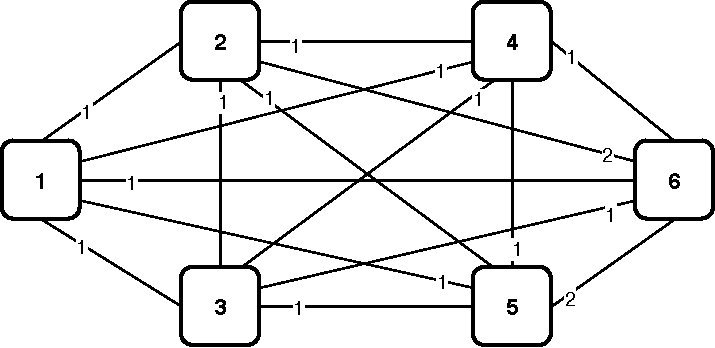
\includegraphics[width=11cm]{sdf/ilp/transparent_survivability/figures/optical_topology_low}
\caption{Optical topology after dimensioning.}
\label{optical2_low}
\end{figure}

In table \ref{link_transp_surv_ref_low} we can see the number of optical channels calculated using \ref{Capex_Link} and \ref{ILPOpaque_CAPEX} and the number of amplifiers for each link calculated using \ref{Capex_amplifiers}.

\begin{table}[h!]
\centering
\begin{tabular}{|| c | c | c ||}
 \hline
 \multicolumn{3}{|| c ||}{Information regarding links} \\
 \hline
 \hline
 Bidirectional Link & Optical Channels & Amplifiers\\
 \hline
 Node 1 <-> Node 2 & 3 & 4 \\
 Node 1 <-> Node 3 & 2 & 6 \\
 Node 2 <-> Node 3 & 3 & 0 \\
 Node 2 <-> Node 4 & 6 & 6 \\
 Node 3 <-> Node 5 & 4 & 8 \\
 Node 4 <-> Node 5 & 1 & 1 \\
 Node 4 <-> Node 6 & 4 & 7 \\
 Node 5 <-> Node 6 & 3 & 3 \\
 \hline
\end{tabular}
\caption{Table with information regarding links for transparent mode.}
\label{link_transp_surv_ref_low}
\end{table}

In table \ref{node_transp_surv_ref_low} we can see the number of line ports and add ports using \ref{OXC_poxc_transparent} the number of long-reach transponders using \ref{EXC_pexc2_transparent} and the number of tributary ports using \ref{EXC_pexc1_transparent}.

\begin{table}[h!]
\centering
\begin{tabular}{|| c | c | c | c | c | c ||}
 \hline
 \multicolumn{6}{|| c ||}{Information regarding nodes} \\
 \hline
 \hline
 \multicolumn{2}{|| c |}{ } & \multicolumn{2}{ c |}{Electrical part} & \multicolumn{2}{ c ||}{Optical part} \\
 \hline
 Node & Resulting Nodal Degree & Tributary Ports & LR Transponders & Add Ports & Line Ports\\
 \hline
 1 & 2 & 29 & 5 & 5 & 5 \\
 2 & 3 & 23 & 6 & 6 & 12 \\
 3 & 3 & 18 & 5 & 5 & 9 \\
 4 & 3 & 20 & 5 & 5 & 11 \\
 5 & 3 & 24 & 6 & 6 & 8 \\
 6 & 2 & 22 & 7 & 7 & 7 \\
\hline
\end{tabular}
\caption{Table with information regarding nodes for transparent mode.}
\label{node_transp_surv_ref_low}
\end{table}

\newpage
Through the information obtained previously on the nodes we can now create tables with detailed information about each node. In each table mentioned below we can see how many ports are connected to a given node and its bit rate (in relation to the line ports and the add ports) and how many ports are assigned to each different bit rate (in relation to the tributary ports).\\

\begin{table}[h!]
\centering
\begin{tabular}{|| c | c | c ||}
 \hline
 \multicolumn{3}{|| c ||}{Detailed description of Node 1} \\
 \hline
 \hline
 Electrical part & Number of total demands & Bit rate \\
 \hline
\multirow{3}{*}{29 tributary ports} & 13 & ODU0 \\
 & 13 & ODU1 \\
 & 3 & ODU2 \\
 \hline
  & Node<--Optical Channels-->Node & Bit rate \\
  \hline
\multirow{5}{*}{5 LR Transponders} & 1  <---- 1 ---->  2 & \multirow{5}{*}{100 Gbits/s} \\
  & 1  <---- 1 ---->  3 & \\
  & 1  <---- 1 ---->  4 & \\
  & 1  <---- 1 ---->  5 & \\
  & 1  <---- 1 ---->  6 & \\
 \hline
 \hline
 Optical part & Node<--Optical Channels-->Node & Bit rate \\
 \hline
 \multirow{5}{*}{5 add ports} & 1  <---- 1 ---->  2 & \multirow{10}{*}{100 Gbits/s} \\
  & 1  <---- 1 ---->  3 & \\
  & 1  <---- 1 ---->  4 & \\
  & 1  <---- 1 ---->  5 & \\
  & 1  <---- 1 ---->  6 & \\ \cline{1-2}
 \multirow{5}{*}{5 line ports} & 1  <---- 1 ---->  2 & \\
  & 1  <---- 1 ---->  3 & \\
  & 1  <---- 1 ---->  4 & \\
  & 1  <---- 1 ---->  5 & \\
  & 1  <---- 1 ---->  6 & \\
\hline
\end{tabular}
\caption{Table with detailed description of node 1. The number of demands is distributed to the various destination nodes, this distribution can be observed in section \ref{low_scenario}. Regarding the number of line ports when this node is equal to the source, it means that add ports are used, otherwise it means that through ports are used. In this node as we can see there are no through ports.}
\end{table}

\newpage
\begin{table}[h!]
\centering
\begin{tabular}{|| c | c | c ||}
 \hline
 \multicolumn{3}{|| c ||}{Detailed description of Node 2} \\
 \hline
 \hline
 Electrical part & Number of total demands & Bit rate \\ \hline
\multirow{5}{*}{23 tributary ports} & 11 & ODU0 \\
 & 7 & ODU1 \\
 & 2 & ODU2 \\
 & 2 & ODU3 \\
 & 1 & ODU4 \\
 \hline
  & Node<--Optical Channels-->Node & Bit rate \\
  \hline
\multirow{5}{*}{6 LR Transponders} & 2  <---- 1 ---->  1 & \multirow{5}{*}{100 Gbits/s} \\
  & 2  <---- 1 ---->  3 & \\
  & 2  <---- 1 ---->  4 & \\
  & 2  <---- 1 ---->  5 & \\
  & 2  <---- 2 ---->  6 & \\
 \hline
 \hline
 Optical part & Node<--Optical Channels-->Node & Bit rate \\
 \hline
 \multirow{5}{*}{6 add ports} & 2  <---- 1 ---->  1 & \multirow{13}{*}{100 Gbits/s} \\
  & 2  <---- 1 ---->  3 & \\
  & 2  <---- 1 ---->  4 & \\
  & 2  <---- 1 ---->  5 & \\
  & 2  <---- 2 ---->  6 & \\ \cline{1-2}
 \multirow{8}{*}{12 line ports} & 2  <---- 1 ---->  1 & \\
  & 2  <---- 1 ---->  3 & \\
  & 2  <---- 1 ---->  4 & \\
  & 2  <---- 1 ---->  5 & \\
  & 2  <---- 2 ---->  6 & \\
  & 1  <---- 1 ---->  4 & \\
  & 1  <---- 1 ---->  6 & \\
  & 3  <---- 1 ---->  4 & \\
\hline
\end{tabular}
\caption{Table with detailed description of node 2. The number of demands is distributed to the various destination nodes, this distribution can be observed in section \ref{low_scenario}. Regarding the number of line ports when this node is equal to the source, it means that add ports are used, otherwise it means that through ports are used. In both cases, the number of ports is double the number of optical channels.}
\end{table}

\newpage
\begin{table}[h!]
\centering
\begin{tabular}{|| c | c | c ||}
 \hline
 \multicolumn{3}{|| c ||}{Detailed description of Node 3} \\
 \hline
 \hline
 Electrical part & Number of total demands & Bit rate \\
 \hline
 \multirow{4}{*}{18 tributary ports} & 7 & ODU0 \\
 & 6 & ODU1\\
 & 3 & ODU2\\
 & 2 & ODU3\\
 \hline
  & Node<--Optical Channels-->Node & Bit rate \\ \hline
 \multirow{5}{*}{5 LR Transponders} & 3  <---- 1 ---->  1 & \multirow{5}{*}{100 Gbits/s} \\
  & 3  <---- 1 ---->  2 & \\
  & 3  <---- 1 ---->  4 & \\
  & 3  <---- 1 ---->  5 & \\
  & 3  <---- 1 ---->  6 & \\
 \hline
 \hline
 Optical part & Node<--Optical Channels-->Node & Bit rate \\
 \hline
 \multirow{5}{*}{5 add ports} & 3  <---- 1 ---->  1 & \multirow{12}{*}{100 Gbits/s} \\
  & 3  <---- 1 ---->  2 & \\
  & 3  <---- 1 ---->  4 & \\
  & 3  <---- 1 ---->  5 & \\
  & 3  <---- 1 ---->  6 & \\ \cline{1-2}
 \multirow{7}{*}{9 line ports} & 3  <---- 1 ---->  1 & \\
  & 3  <---- 1 ---->  2 & \\
  & 3  <---- 1 ---->  4 & \\
  & 3  <---- 1 ---->  5 & \\
  & 3  <---- 1 ---->  6 & \\
  & 1  <---- 1 ---->  5 & \\
  & 2  <---- 1 ---->  5 & \\
\hline
\end{tabular}
\caption{Table with detailed description of node 3. The number of demands is distributed to the various destination nodes, this distribution can be observed in section \ref{low_scenario}. Regarding the number of line ports when this node is equal to the source, it means that add ports are used, otherwise it means that through ports are used. In the latter the number of ports is double the number of optical channels.}
\end{table}

\newpage
\begin{table}[h!]
\centering
\begin{tabular}{|| c | c | c ||}
 \hline
 \multicolumn{3}{|| c ||}{Detailed description of Node 4} \\
 \hline
 \hline
 Electrical part & Number of total demands & Bit rate \\ \hline
\multirow{3}{*}{20 tributary ports} & 7 & ODU0 \\
 & 10 & ODU1 \\
 & 3 & ODU2 \\
 \hline
  & Node<--Optical Channels-->Node & Bit rate \\ \hline
 \multirow{5}{*}{5 LR Transponders} & 4  <---- 1 ---->  1 & \multirow{5}{*}{100 Gbits/s} \\
  & 4  <---- 1 ---->  2 & \\
  & 4  <---- 1 ---->  3 & \\
  & 4  <---- 1 ---->  5 & \\
  & 4  <---- 1 ---->  6 & \\
 \hline
 \hline
 Optical part & Node<--Optical Channels-->Node & Bit rate \\
 \hline
 \multirow{5}{*}{5 add ports} & 4  <---- 1 ---->  1 & \multirow{12}{*}{100 Gbits/s} \\
  & 4  <---- 1 ---->  2 & \\
  & 4  <---- 1 ---->  3 & \\
  & 4  <---- 1 ---->  5 & \\
  & 4  <---- 1 ---->  6 & \\ \cline{1-2}
 \multirow{7}{*}{11 line ports} & 4  <---- 1 ---->  1 & \\
  & 4  <---- 1 ---->  2 & \\
  & 4  <---- 1 ---->  3 & \\
  & 4  <---- 1 ---->  5 & \\
  & 4  <---- 1 ---->  6 & \\
  & 1  <---- 1 ---->  6 & \\
  & 2  <---- 2 ---->  6 & \\
\hline
\end{tabular}
\caption{Table with detailed description of node 4. The number of demands is distributed to the various destination nodes, this distribution can be observed in section \ref{low_scenario}. Regarding the number of line ports when this node is equal to the source, it means that add ports are used, otherwise it means that through ports are used. In the latter the number of ports is double the number of optical channels.}
\end{table}

\newpage
\begin{table}[h!]
\centering
\begin{tabular}{|| c | c | c ||}
 \hline
 \multicolumn{3}{|| c ||}{Detailed description of Node 5} \\
 \hline
 \hline
 Electrical part & Number of total demands & Bit rate \\ \hline
\multirow{5}{*}{24 tributary ports} & 14 & ODU0 \\
 & 4 & ODU1 \\
 & 4 & ODU2 \\
 & 1 & ODU3 \\
 & 1 & ODU4 \\
 \hline
  & Node<--Optical Channels-->Node & Bit rate \\ \hline
 \multirow{5}{*}{6 LR Trasponders} & 5  <---- 1 ---->  1 & \multirow{5}{*}{100 Gbits/s} \\
  & 5  <---- 1 ---->  2 & \\
  & 5  <---- 1 ---->  3 & \\
  & 5  <---- 1 ---->  4 & \\
  & 5  <---- 2 ---->  6 & \\
 \hline
 \hline
 Optical part & Node<--Optical Channels-->Node & Bit rate \\
 \hline
 \multirow{5}{*}{6 add ports} & 5  <---- 1 ---->  1 & \multirow{11}{*}{100 Gbits/s} \\
  & 5  <---- 1 ---->  2 & \\
  & 5  <---- 1 ---->  3 & \\
  & 5  <---- 1 ---->  4 & \\
  & 5  <---- 2 ---->  6 & \\ \cline{1-2}
 \multirow{6}{*}{8 line ports} & 5  <---- 1 ---->  1 & \\
  & 5  <---- 1 ---->  2 & \\
  & 5  <---- 1 ---->  3 & \\
  & 5  <---- 1 ---->  4 & \\
  & 5  <---- 2 ---->  6 & \\
  & 3  <---- 1 ---->  6 &\\
\hline
\end{tabular}
\caption{Table with detailed description of node 5. The number of demands is distributed to the various destination nodes, this distribution can be observed in section \ref{low_scenario}. Regarding the number of line ports when this node is equal to the source, it means that add ports are used, otherwise it means that through ports are used. In the latter the number of ports is double the number of optical channels.}
\end{table}

\newpage
\begin{table}[h!]
\centering
\begin{tabular}{|| c | c | c ||}
 \hline
 \multicolumn{3}{|| c ||}{Detailed description of Node 6} \\
 \hline
 \hline
 Electrical part & Number of total demands & Bit rate \\ \hline
\multirow{5}{*}{22 tributary ports} & 8 & ODU0 \\
 & 10 & ODU1 \\
 & 1 & ODU2 \\
 & 1 & ODU3 \\
 & 2 & ODU4 \\
 \hline
  & Node<--Optical Channels-->Node & Bit rate \\ \hline
 \multirow{5}{*}{7 LR Transponders} & 6  <---- 1 ---->  1 & \\
  & 6  <---- 2 ---->  2 & \\
  & 6  <---- 1 ---->  3 & \\
  & 6  <---- 1 ---->  4 & \\
  & 6  <---- 2 ---->  5 & \\
 \hline
 Optical part & Node<--Optical Channels-->Node & Bit rate \\
 \hline
 \multirow{5}{*}{7 add ports} & 6  <---- 1 ---->  1 & \multirow{10}{*}{100 Gbits/s} \\
  & 6  <---- 2 ---->  2 & \\
  & 6  <---- 1 ---->  3 & \\
  & 6  <---- 1 ---->  4 & \\
  & 6  <---- 2 ---->  5 & \\ \cline{1-2}
 \multirow{5}{*}{7 line ports} & 6  <---- 1 ---->  1 & \\
  & 6  <---- 2 ---->  2 & \\
  & 6  <---- 1 ---->  3 & \\
  & 6  <---- 1 ---->  4 & \\
  & 6  <---- 2 ---->  5 & \\
\hline
\end{tabular}
\caption{Table with detailed description of node 6. The number of demands is distributed to the various destination nodes, this distribution can be observed in section \ref{low_scenario}. Regarding the number of line ports when this node is equal to the source, it means that add ports are used, otherwise it means that through ports are used.  In this node as we can see there are no through ports.}
\end{table}

\vspace{17pt}
Now, in next page, let's focus on the routing information in table \ref{path_transp_surv_ref_low}. These paths are bidirectional so the path from one node to another is the same path in the opposite direction.\\
\newpage
\begin{table}[h!]
\centering
\begin{tabular}{|| c | c | c ||}
 \hline
 \multicolumn{3}{|| c ||}{Routing} \\
 \hline
 \hline
 o & d & Links \\
 \hline
 1 & 2 & \{(1,2)\} \\ \hline
 1 & 3 & \{(1,3)\} \\ \hline
 1 & 4 & \{(1,2),(2,4)\}\\ \hline
 1 & 5 & \{(1,3),(3,5)\}\\ \hline
 1 & 6 & \{(1,2),(2,4),(4,6)\}\\ \hline
 2 & 3 & \{(2,3)\}\\ \hline
 2 & 4 & \{(2,4)\}\\ \hline
 2 & 5 & \{(2,3),(3,5)\}\\ \hline
 2 & 6 & \{(2,4),(4,6)\}\\ \hline
 3 & 4 & \{(3,2),(2,4)\}\\ \hline
 3 & 5 & \{(3,5)\}\\ \hline
 3 & 6 & \{(3,5),(5,6)\}\\ \hline
 4 & 5 & \{(4,5)\}\\ \hline
 4 & 6 & \{(4,6)\}\\ \hline
 5 & 6 & \{(5,6)\}\\
 \hline
\end{tabular}
\caption{Table with description of routing.}
\label{path_transp_surv_ref_low}
\end{table}

Finally and most importantly through table \ref{scripttransp_surv_ref_low} we can see the CAPEX result for this model. This value is obtained using equation \ref{ILPOpaque_CAPEX} and all of the constraints mentioned above.\\

\begin{table}[h!]
\centering
\begin{tabular}{|| c | c | c | c | c | c | c ||}
 \hline
 \multicolumn{7}{|| c ||}{CAPEX of the Network} \\
 \hline
 \hline
 \multicolumn{3}{|| c |}{ } & Quantity & Unit Price & Cost & Total \\
 \hline
 \multirow{3}{*}{Link Cost} & \multicolumn{2}{ c |}{OLTs} & 16 & 15 000 \euro & 240 000 \euro & \multirow{3}{*}{26 520 000 \euro} \\ \cline{2-6}
 & \multicolumn{2}{ c |}{100 Gbits/s Transceivers} & 52 & 5 000 \euro/Gbit/s & 26 000 000 \euro & \\ \cline{2-6}
 & \multicolumn{2}{ c |}{Amplifiers} & 70 & 4 000 \euro & 280 000 \euro & \\
 \hline
 \multirow{10}{*}{Node Cost} & \multirow{7}{*}{Electrical} & EXCs & 6 & 10 000 \euro & 60 000 \euro & \multirow{10}{*}{3 797 590 \euro} \\ \cline{3-6}
 & & ODU0 Ports & 60 & 10 \euro/port & 600 \euro & \\ \cline{3-6}
 & & ODU1 Ports & 50 & 15 \euro/port & 750 \euro & \\ \cline{3-6}
 & & ODU2 Ports & 16 & 30 \euro/port & 480 \euro & \\ \cline{3-6}
 & & ODU3 Ports & 6 & 60 \euro/port & 360 \euro & \\ \cline{3-6}
 & & ODU4 Ports & 4 & 100 \euro/port & 400 \euro & \\ \cline{3-6}
 & &Transponders& 34 & 100 000 \euro/port & 3 400 000 \euro & \\ \cline{2-6}
 & \multirow{3}{*}{Optical} & OXCs & 6 & 20 000 \euro & 120 000 \euro & \\ \cline{3-6}
 & & Line Ports & 52 & 2 500 \euro/port & 130 000 \euro & \\ \cline{3-6}
 & & Add Ports & 34 & 2 500 \euro/port & 85 000 \euro & \\
 \hline
 \multicolumn{6}{|| c |}{Total Network Cost} & 30 317 590 \euro \\
\hline
\end{tabular}
\caption{Table with detailed description of CAPEX for this scenario.}
\label{scripttransp_surv_ref_low}
\end{table}

\newpage
All the values calculated in the previous table were obtained through the equations \ref{Capex_Link} and \ref{Capex_Node} referred to in section \ref{ILP_CAPEX}, but for a more detailed analysis we created table \ref{formulas_transp} where we can see how all the parameters are calculated individually.\\

\begin{table}[h!]
\centering
\begin{tabular}{|| c | c ||}
 \hline
  & Equation used to calculate the cost \\ \hline
 OLTs & \(\displaystyle 2 \sum_{i=1}^{N}\sum_{j=i+1}^{N} L_{ij} \gamma_0^{OLT} \) \\ \hline
 Transceivers & \(\displaystyle 2 \sum_{i=1}^{N}\sum_{j=i+1}^{N} L_{ij} f_{ij}^{od} \gamma_1^{OLT} \tau \) \\ \hline
 Amplifiers & \(\displaystyle 2 \sum_{i=1}^{N}\sum_{j=i+1}^{N} L_{ij} N^R_{ij} c^R \) \\ \hline
 EXCs & \(\displaystyle \sum_{n=1}^N N_{exc,n} \gamma_{e0} \) \\ \hline
 ODU0 Port & \(\displaystyle \sum_{n=1}^{N} \sum_{d=1}^{N} N_{exc,n} D_{nd,0} \gamma_{e1,0} \) \\ \hline
 ODU1 Port & \(\displaystyle \sum_{n=1}^{N} \sum_{d=1}^{N} N_{exc,n} D_{nd,1} \gamma_{e1,1} \) \\ \hline
 ODU2 Port & \(\displaystyle \sum_{n=1}^{N} \sum_{d=1}^{N} N_{exc,n} D_{nd,2} \gamma_{e1,2} \)\\ \hline
 ODU3 Port & \(\displaystyle \sum_{n=1}^{N} \sum_{d=1}^{N} N_{exc,n} D_{nd,3} \gamma_{e1,3} \) \\ \hline
 ODU4 Port & \(\displaystyle \sum_{n=1}^{N} \sum_{d=1}^{N} N_{exc,n} D_{nd,4} \gamma_{e1,4} \) \\ \hline
 LR Transponders & \(\displaystyle \sum_{n=1}^{N} \sum_{j=1}^{N} N_{exc,n} \lambda_{od} \gamma_{e1,-1} \) \\ \hline
 OXCs & \(\displaystyle \sum_{n=1}^N N_{oxc,n} \gamma_{o0} \) \\ \hline
 Add Port & \(\displaystyle \sum_{n=1}^{N} \sum_{j=1}^{N} N_{oxc,n} \lambda_{od} \gamma_{o1} \) \\ \hline
 Line Port & \(\displaystyle \sum_{n=1}^{N} \sum_{j=1}^{N} N_{oxc,n} f_{ij}^{od} \gamma_{o1} \) \\ \hline
 CAPEX & The final cost is calculated by summing all previous results. \\
 \hline
 \end{tabular}
\caption{Table with description of calculation}
\label{formulas_transp}
\end{table}

\newpage
\textbf{Medium Traffic Scenario:}\\

In this scenario we have to take into account the traffic calculated in \ref{medium_traffic_scenario}. In a first phase we will show the various existing topologies of the network. The first are the allowed topologies, physical and optical topology, the second are the logical topology for all ODUs and finally the resulting physical and optical topology.\\

\begin{figure}[h!]
\centering
\includegraphics[width=12cm]{sdf/ilp/transparent_survivability/figures/allowed_physical_topology}
\caption{Allowed physical topology. The allowed physical topology is defined by the duct and sites in the field. It is assumed that each duct supports up to 1 bidirectional transmission system and each site supports up to 1 node.}
\label{allowed2_physical_medium}
\end{figure}

\vspace{11pt}
\begin{figure}[h!]
\centering
\includegraphics[width=12cm]{sdf/ilp/transparent_survivability/figures/allowed_optical_topology}
\caption{Allowed optical topology. The allowed optical topology is defined by the transport mode (transparent transport mode in this case). It is assumed that each connections between demands supports up to 100 lightpaths.}
\label{allowed2_optical_medium}
\end{figure}

\newpage
\begin{figure}[h!]
\centering
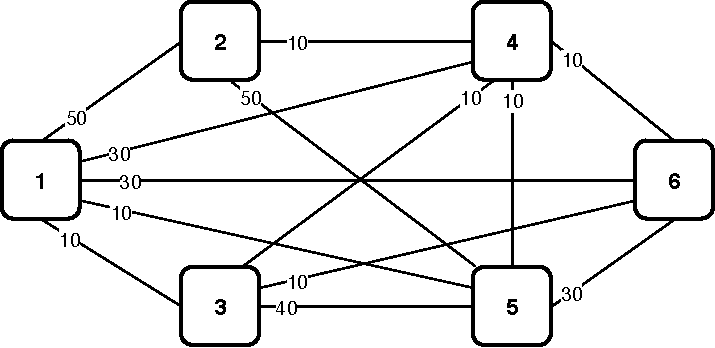
\includegraphics[width=12cm]{sdf/ilp/transparent_survivability/figures/logical_topology_ODU0_medium}
\caption{ODU0 logical topology defined by the ODU0 traffic matrix.}
\label{logical2_ODU0_medium}
\end{figure}

\begin{figure}[h!]
\centering
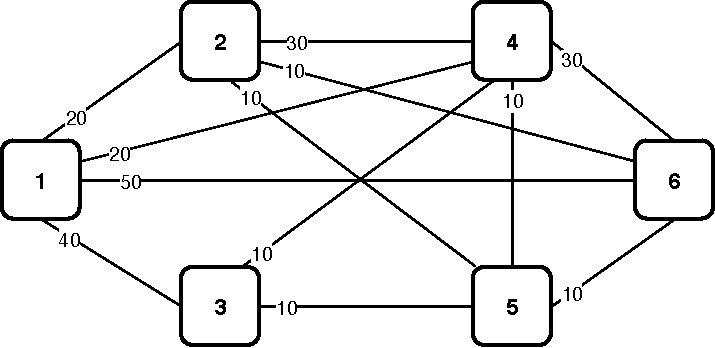
\includegraphics[width=12cm]{sdf/ilp/transparent_survivability/figures/logical_topology_ODU1_medium}
\caption{ODU1 logical topology defined by the ODU1 traffic matrix.}
\label{logical2_ODU1_medium}
\end{figure}

\begin{figure}[h!]
\centering
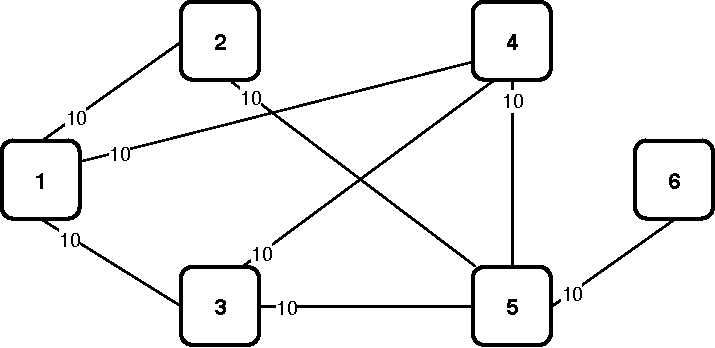
\includegraphics[width=12cm]{sdf/ilp/transparent_survivability/figures/logical_topology_ODU2_medium}
\caption{ODU2 logical topology defined by the ODU2 traffic matrix.}
\label{logical2_ODU2_medium}
\end{figure}

\begin{figure}[h!]
\centering
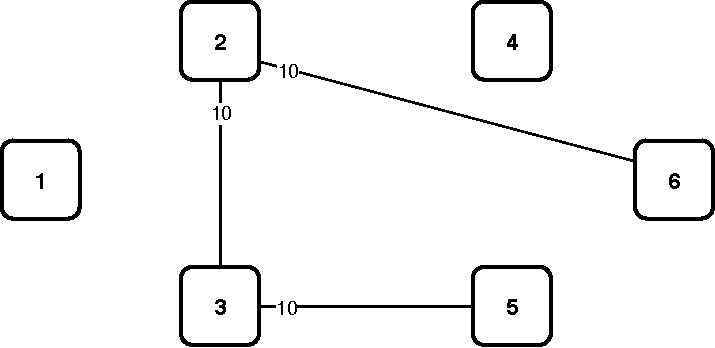
\includegraphics[width=12cm]{sdf/ilp/transparent_survivability/figures/logical_topology_ODU3_medium}
\caption{ODU3 logical topology defined by the ODU3 traffic matrix.}
\label{logical2_ODU3_medium}
\end{figure}

\begin{figure}[h!]
\centering
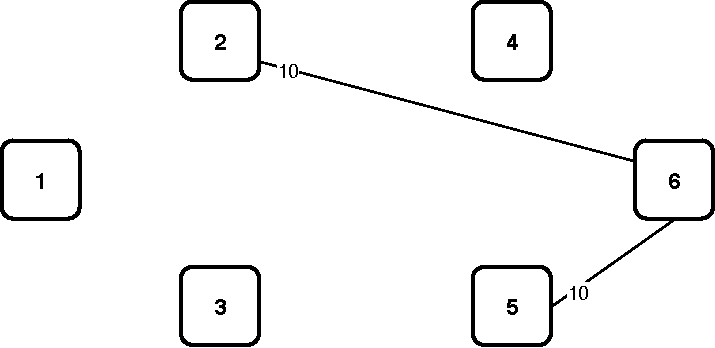
\includegraphics[width=12cm]{sdf/ilp/transparent_survivability/figures/logical_topology_ODU4_medium}
\caption{ODU4 logical topology defined by the ODU4 traffic matrix.}
\label{logical2_ODU4_medium}
\end{figure}

\begin{figure}[h!]
\centering
\includegraphics[width=12cm]{sdf/ilp/transparent_survivability/figures/physical_topology}
\caption{Physical topology after dimensioning.}
\label{physical2_medium}
\end{figure}
\newpage
\begin{figure}[h!]
\centering
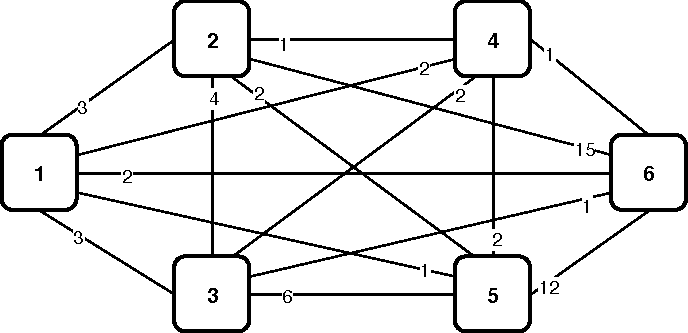
\includegraphics[width=11cm]{sdf/ilp/transparent_survivability/figures/optical_topology_medium}
\caption{Optical topology after dimensioning.}
\label{optical2_medium}
\end{figure}

In table \ref{link_transp_surv_ref_medium} we can see the number of optical channels calculated using \ref{Capex_Link} and \ref{ILPOpaque_CAPEX} and the number of amplifiers for each link calculated using \ref{Capex_amplifiers}.

\begin{table}[h!]
\centering
\begin{tabular}{|| c | c | c ||}
 \hline
 \multicolumn{3}{|| c ||}{Information regarding links} \\
 \hline
 \hline
 Bidirectional Link & Optical Channels & Amplifiers\\
 \hline
 Node 1 <-> Node 2 & 7 & 4 \\
 Node 1 <-> Node 3 & 4 & 6 \\
 Node 2 <-> Node 3 & 8 & 0 \\
 Node 2 <-> Node 4 & 22 & 6 \\
 Node 3 <-> Node 5 & 10 & 8 \\
 Node 4 <-> Node 5 & 2 & 1 \\
 Node 4 <-> Node 6 & 18 & 7 \\
 Node 5 <-> Node 6 & 13 & 3 \\
 \hline
\end{tabular}
\caption{Table with information regarding links for transparent mode.}
\label{link_transp_surv_ref_medium}
\end{table}

In table \ref{node_transp_surv_ref_medium} we can see the number of line ports and add ports using \ref{OXC_poxc_transparent} the number of long-reach transponders using \ref{EXC_pexc2_transparent} and the number of tributary ports using \ref{EXC_pexc1_transparent}.

\begin{table}[h!]
\centering
\begin{tabular}{|| c | c | c | c | c | c ||}
 \hline
 \multicolumn{6}{|| c ||}{Information regarding nodes} \\
 \hline
 \hline
 \multicolumn{2}{|| c |}{ } & \multicolumn{2}{ c |}{Electrical part} & \multicolumn{2}{ c ||}{Optical part} \\
 \hline
 Node & Resulting Nodal Degree & Tributary Ports & LR Transponders & Add Ports & Line Ports\\
 \hline
 1 & 2 & 290 & 11 & 11 & 11 \\
 2 & 3 & 230 & 25 & 25 & 37 \\
 3 & 3 & 180 & 16 & 16 & 22 \\
 4 & 3 & 200 & 8 & 8 & 42 \\
 5 & 3 & 240 & 23 & 23 & 25 \\
 6 & 2 & 220 & 31 & 31 & 31 \\
\hline
\end{tabular}
\caption{Table with information regarding nodes for transparent mode.}
\label{node_transp_surv_ref_medium}
\end{table}

\newpage
Through the information obtained previously on the nodes we can now create tables with detailed information about each node. In each table mentioned below we can see how many ports are connected to a given node and its bit rate (in relation to the line ports and the add ports) and how many ports are assigned to each different bit rate (in relation to the tributary ports).\\

\begin{table}[h!]
\centering
\begin{tabular}{|| c | c | c ||}
 \hline
 \multicolumn{3}{|| c ||}{Detailed description of Node 1} \\
 \hline
 \hline
 Electrical part & Number of total demands & Bit rate \\ \hline
\multirow{3}{*}{290 tributary ports} & 130 & ODU0 \\
 & 130 & ODU1 \\
 & 30 & ODU2 \\
 \hline
  & Node<--Optical Channels-->Node & Bit rate \\ \hline
 \multirow{5}{*}{11 LR Transponders} & 1  <---- 3 ---->  2 & \multirow{5}{*}{100 Gbits/s} \\
  & 1  <---- 3 ---->  3 & \\
  & 1  <---- 2 ---->  4 & \\
  & 1  <---- 1 ---->  5 & \\
  & 1  <---- 2 ---->  6 & \\
 \hline
 \hline
 Optical part & Node<--Optical Channels-->Node & Bit rate \\
 \hline
 \multirow{5}{*}{11 add ports} & 1  <---- 3 ---->  2 & \multirow{10}{*}{100 Gbits/s} \\
  & 1  <---- 3 ---->  3 & \\
  & 1  <---- 2 ---->  4 & \\
  & 1  <---- 1 ---->  5 & \\
  & 1  <---- 2 ---->  6 & \\ \cline{1-2}
 \multirow{5}{*}{11 line ports} & 1  <---- 3 ---->  2 & \\
  & 1  <---- 3 ---->  3 & \\
  & 1  <---- 2 ---->  4 & \\
  & 1  <---- 1 ---->  5 & \\
  & 1  <---- 2 ---->  6 & \\
\hline
\end{tabular}
\caption{Table with detailed description of node 1. The number of demands is distributed to the various destination nodes, this distribution can be observed in section \ref{medium_traffic_scenario} . Regarding the number of line ports when this node is equal to the source, it means that add ports are used, otherwise it means that through ports are used.  In this node as we can see there are no through ports.}
\end{table}

\newpage
\begin{table}[h!]
\centering
\begin{tabular}{|| c | c | c ||}
 \hline
 \multicolumn{3}{|| c ||}{Detailed description of Node 2} \\
 \hline
 \hline
 Electrical part & Number of total demands & Bit rate \\ \hline
\multirow{5}{*}{230 tributary ports} & 110 & ODU0 \\
 & 70 & ODU1 \\
 & 20 & ODU2 \\
 & 20 & ODU3 \\
 & 10 & ODU4 \\
 \hline
  & Node<--Optical Channels-->Node & Bit rate \\
 \hline
 \multirow{5}{*}{25 LR Transponders} & 2  <---- 3 ---->  1 & \multirow{5}{*}{100 Gbits/s} \\
  & 2  <---- 4 ---->  3 & \\
  & 2  <---- 1 ---->  4 & \\
  & 2  <---- 2 ---->  5 & \\
  & 2  <---- 15 ---->  6 & \\
 \hline
 \hline
 Optical part & Node<--Optical Channels-->Node & Bit rate \\
 \hline
 \multirow{5}{*}{25 add ports} & 2  <---- 3 ---->  1 & \multirow{13}{*}{100 Gbits/s} \\
  & 2  <---- 4 ---->  3 & \\
  & 2  <---- 1 ---->  4 & \\
  & 2  <---- 2 ---->  5 & \\
  & 2  <---- 15 ---->  6 & \\ \cline{1-2}
 \multirow{8}{*}{37 line ports} & 2  <---- 3 ---->  1 & \\
  & 2  <---- 4 ---->  3 & \\
  & 2  <---- 1 ---->  4 & \\
  & 2  <---- 2 ---->  5 & \\
  & 2  <---- 15 ---->  6 & \\
  & 1  <---- 2 ---->  4 & \\
  & 1  <---- 2 ---->  6 & \\
  & 3  <---- 2 ---->  4 & \\
\hline
\end{tabular}
\caption{Table with detailed description of node 2. The number of demands is distributed to the various destination nodes, this distribution can be observed in section \ref{medium_traffic_scenario} . Regarding the number of line ports when this node is equal to the source, it means that add ports are used, otherwise it means that through ports are used. In the latter the number of ports is double the number of optical channels.}
\end{table}

\newpage
\begin{table}[h!]
\centering
\begin{tabular}{|| c | c | c ||}
 \hline
 \multicolumn{3}{|| c ||}{Detailed description of Node 3} \\
 \hline
 \hline
 Electrical part & Number of total demands & Bit rate \\ \hline
\multirow{4}{*}{180 tributary ports} & 70 & ODU0 \\
 & 60 & ODU1\\
 & 30 & ODU2\\
 & 20 & ODU3\\
 \hline
  & Node<--Optical Channels-->Node & Bit rate \\
 \hline
 \multirow{5}{*}{16 LR Transponders} & 3  <---- 3 ---->  1 & \multirow{5}{*}{100 Gbits/s} \\
  & 3  <---- 4 ---->  2 & \\
  & 3  <---- 2 ---->  4 & \\
  & 3  <---- 6 ---->  5 & \\
  & 3  <---- 1 ---->  6 & \\
 \hline
 \hline
 Optical part & Node<--Optical Channels-->Node & Bit rate \\
 \hline
 \multirow{5}{*}{16 add ports} & 3  <---- 3 ---->  1 & \multirow{12}{*}{100 Gbits/s}  \\
  & 3  <---- 4 ---->  2 & \\
  & 3  <---- 2 ---->  4 & \\
  & 3  <---- 6 ---->  5 & \\
  & 3  <---- 1 ---->  6 & \\ \cline{1-2}
 \multirow{7}{*}{22 line ports} & 3  <---- 3 ---->  1 & \\
  & 3  <---- 4 ---->  2 & \\
  & 3  <---- 2 ---->  4 & \\
  & 3  <---- 6 ---->  5 & \\
  & 3  <---- 1 ---->  6 & \\
  & 1  <---- 1 ---->  5 & \\
  & 2  <---- 2 ---->  5 & \\
\hline
\end{tabular}
\caption{Table with detailed description of node 3. The number of demands is distributed to the various destination nodes, this distribution can be observed in section \ref{medium_traffic_scenario} . Regarding the number of line ports when this node is equal to the source, it means that add ports are used, otherwise it means that through ports are used. In the latter the number of ports is double the number of optical channels.}
\end{table}

\newpage
\begin{table}[h!]
\centering
\begin{tabular}{|| c | c | c ||}
 \hline
 \multicolumn{3}{|| c ||}{Detailed description of Node 4} \\
 \hline
 \hline
 Electrical part & Number of total demands & Bit rate \\ \hline
\multirow{3}{*}{200 tributary ports} & 70 & ODU0 \\
 & 100 & ODU1 \\
 & 30 & ODU2 \\
 \hline
  & Node<--Optical Channels-->Node & Bit rate \\
 \hline
 \multirow{5}{*}{8 add ports} & 4  <---- 2 ---->  1 & \multirow{5}{*}{100 Gbits/s} \\
  & 4  <---- 1 ---->  2 & \\
  & 4  <---- 2 ---->  3 & \\
  & 4  <---- 2 ---->  5 & \\
  & 4  <---- 1 ---->  6 & \\
 \hline
 Optical part & Node<--Optical Channels-->Node & Bit rate \\
 \hline
 \multirow{5}{*}{8 add ports} & 4  <---- 2 ---->  1 & \multirow{12}{*}{100 Gbits/s} \\
  & 4  <---- 1 ---->  2 & \\
  & 4  <---- 2 ---->  3 & \\
  & 4  <---- 2 ---->  5 & \\
  & 4  <---- 1 ---->  6 & \\ \cline{1-2}
 \multirow{7}{*}{42 line ports} & 4  <---- 2 ---->  1 & \\
  & 4  <---- 1 ---->  2 & \\
  & 4  <---- 2 ---->  3 & \\
  & 4  <---- 2 ---->  5 & \\
  & 4  <---- 1 ---->  6 & \\
  & 1  <---- 2 ---->  6 & \\
  & 2  <---- 15 ---->  6 & \\
\hline
\end{tabular}
\caption{Table with detailed description of node 4. The number of demands is distributed to the various destination nodes, this distribution can be observed in section \ref{medium_traffic_scenario} . Regarding the number of line ports when this node is equal to the source, it means that add ports are used, otherwise it means that through ports are used. In the latter the number of ports is double the number of optical channels.}
\end{table}

\newpage
\begin{table}[h!]
\centering
\begin{tabular}{|| c | c | c ||}
 \hline
 \multicolumn{3}{|| c ||}{Detailed description of Node 5} \\
 \hline
 \hline
 Electrical part & Number of total demands & Bit rate \\ \hline
\multirow{5}{*}{240 tributary ports} & 140 & ODU0 \\
 & 40 & ODU1 \\
 & 40 & ODU2 \\
 & 10 & ODU3 \\
 & 10 & ODU4 \\
 \hline
  & Node<--Optical Channels-->Node & Bit rate \\
 \hline
 \multirow{5}{*}{23 LR Transponders} & 5  <---- 1 ---->  1 & \multirow{5}{*}{100 Gbits/s}\\
  & 5  <---- 2 ---->  2 & \\
  & 5  <---- 6 ---->  3 & \\
  & 5  <---- 2 ---->  4 & \\
  & 5  <---- 12 ---->  6 & \\
 \hline
 \hline
 Optical part & Node<--Optical Channels-->Node & Bit rate \\
 \hline
 \multirow{5}{*}{23 add ports} & 5  <---- 1 ---->  1 & \multirow{11}{*}{100 Gbits/s} \\
  & 5  <---- 2 ---->  2 & \\
  & 5  <---- 6 ---->  3 & \\
  & 5  <---- 2 ---->  4 & \\
  & 5  <---- 12 ---->  6 & \\ \cline{1-2}
 \multirow{6}{*}{25 line ports} & 5  <---- 1 ---->  1 & \\
  & 5  <---- 2 ---->  2 & \\
  & 5  <---- 6 ---->  3 & \\
  & 5  <---- 2 ---->  4 & \\
  & 5  <---- 12 ---->  6 & \\
  & 3  <---- 1 ---->  6 & \\
\hline
\end{tabular}
\caption{Table with detailed description of node 5. The number of demands is distributed to the various destination nodes, this distribution can be observed in section \ref{medium_traffic_scenario} . Regarding the number of line ports when this node is equal to the source, it means that add ports are used, otherwise it means that through ports are used. In the latter the number of ports is double the number of optical channels.}
\end{table}

\newpage
\begin{table}[h!]
\centering
\begin{tabular}{|| c | c | c ||}
 \hline
 \multicolumn{3}{|| c ||}{Detailed description of Node 6} \\
 \hline
 \hline
 Electrical part & Number of total demands & Bit rate \\ \hline
\multirow{5}{*}{220 tributary ports} & 80 & ODU0 \\
 & 100 & ODU1 \\
 & 10 & ODU2 \\
 & 10 & ODU3 \\
 & 20 & ODU4 \\
 \hline
  & Node<--Optical Channels-->Node & Bit rate \\
 \hline
 \multirow{5}{*}{31 LR Transponders} & 6  <---- 2 ---->  1 & \multirow{5}{*}{100 Gbits/s} \\
  & 6  <---- 15 ---->  2 & \\
  & 6  <---- 1 ---->  3 & \\
  & 6  <---- 1 ---->  4 & \\
  & 6  <---- 12 ---->  5 & \\
 \hline
 \hline
 Optical part & Node<--Optical Channels-->Node & Bit rate \\
 \hline
 \multirow{5}{*}{31 add ports} & 6  <---- 2 ---->  1 & \multirow{10}{*}{100 Gbits/s} \\
  & 6  <---- 15 ---->  2 & \\
  & 6  <---- 1 ---->  3 & \\
  & 6  <---- 1 ---->  4 & \\
  & 6  <---- 12 ---->  5 & \\ \cline{1-2}
 \multirow{3}{*}{31 line ports} & 6  <---- 2 ---->  1 & \\
  & 6  <---- 15 ---->  2 & \\
  & 6  <---- 1 ---->  3 & \\
  & 6  <---- 1 ---->  4 & \\
  & 6  <---- 12 ---->  5 & \\
\hline
\end{tabular}
\caption{Table with detailed description of node 6. The number of demands is distributed to the various destination nodes, this distribution can be observed in section \ref{medium_traffic_scenario} . Regarding the number of line ports when this node is equal to the source, it means that add ports are used, otherwise it means that through ports are used.  In this node as we can see there are no through ports.}
\end{table}

\vspace{17pt}
Now, in next page, let's focus on the routing information in table \ref{path_transp_surv_ref_medium}. These paths are bidirectional so the path from one node to another is the same path in the opposite direction.\\
\newpage
\begin{table}[h!]
\centering
\begin{tabular}{|| c | c | c ||}
 \hline
 \multicolumn{3}{|| c ||}{Routing} \\
 \hline
 \hline
 o & d & Links \\
 \hline
 1 & 2 & \{(1,2)\} \\ \hline
 1 & 3 & \{(1,3)\} \\ \hline
 1 & 4 & \{(1,2),(2,4)\}\\ \hline
 1 & 5 & \{(1,3),(3,5)\}\\ \hline
 1 & 6 & \{(1,2),(2,4),(4,6)\}\\ \hline
 2 & 3 & \{(2,3)\}\\ \hline
 2 & 4 & \{(2,4)\}\\ \hline
 2 & 5 & \{(2,3),(3,5)\}\\ \hline
 2 & 6 & \{(2,4),(4,6)\}\\ \hline
 3 & 4 & \{(3,2),(2,4)\}\\ \hline
 3 & 5 & \{(3,5)\}\\ \hline
 3 & 6 & \{(3,5),(5,6)\}\\ \hline
 4 & 5 & \{(4,5)\}\\ \hline
 4 & 6 & \{(4,6)\}\\ \hline
 5 & 6 & \{(5,6)\}\\
 \hline
\end{tabular}
\caption{Table with description of routing}
\label{path_transp_surv_ref_medium}
\end{table}

Finally and most importantly through table \ref{scripttransp_surv_ref_medium} we can see the CAPEX result for this model. This value is obtained using equation \ref{ILPOpaque_CAPEX} and all of the constraints mentioned above. In table \ref{formulas_transp} mentioned in previous scenario we can see how all the values were calculated.

\begin{table}[h!]
\centering
\begin{tabular}{|| c | c | c | c | c | c | c ||}
 \hline
 \multicolumn{7}{|| c ||}{CAPEX of the Network} \\
 \hline
 \hline
 \multicolumn{3}{|| c |}{ } & Quantity & Unit Price & Cost & Total \\
 \hline
 \multirow{3}{*}{Link Cost} & \multicolumn{2}{ c |}{OLTs} & 16 & 15 000 \euro & 240 000 \euro & \multirow{3}{*}{84 520 000 \euro} \\ \cline{2-6}
 & \multicolumn{2}{ c |}{100 Gbits/s Transceivers} & 168 & 5 000 \euro/Gbit/s & 84 000 000 \euro & \\ \cline{2-6}
 & \multicolumn{2}{ c |}{Amplifiers} & 70 & 4 000 \euro & 280 000 \euro & \\
 \hline
 \multirow{10}{*}{Node Cost} & \multirow{7}{*}{Electrical} & EXCs & 6 & 10 000 \euro & 60 000 \euro & \multirow{10}{*}{12 310 900 \euro} \\ \cline{3-6}
 & & ODU0 Ports & 600 & 10 \euro/port & 6 000 \euro & \\ \cline{3-6}
 & & ODU1 Ports & 500 & 15 \euro/port & 7 500 \euro & \\ \cline{3-6}
 & & ODU2 Ports & 160 & 30 \euro/port & 4 800 \euro & \\ \cline{3-6}
 & & ODU3 Ports & 60 & 60 \euro/port & 3 600 \euro & \\ \cline{3-6}
 & & ODU4 Ports & 40 & 100 \euro/port & 4 000 \euro & \\ \cline{3-6}
 & &Transponders& 114 & 100 000 \euro/port & 11 400 000 \euro & \\ \cline{2-6}
 & \multirow{3}{*}{Optical} & OXCs & 6 & 20 000 \euro & 120 000 \euro & \\ \cline{3-6}
 & & Line Ports & 168 & 2 500 \euro/port & 420 000 \euro & \\ \cline{3-6}
 & & Add Ports & 114 & 2 500 \euro/port & 285 000 \euro & \\
 \hline
 \multicolumn{6}{|| c |}{Total Network Cost} &96 830 900 \euro \\
\hline
\end{tabular}
\caption{Table with detailed description of CAPEX}
\label{scripttransp_surv_ref_medium}
\end{table}

\newpage
\textbf{High Traffic Scenario:}\\

In this scenario we have to take into account the traffic calculated in \ref{high_traffic_scenario}. In a first phase we will show the various existing topologies of the network. The first are the allowed topologies, physical and optical topology, the second are the logical topology for all ODUs and finally the resulting physical and optical topology.\\

\begin{figure}[h!]
\centering
\includegraphics[width=12cm]{sdf/ilp/transparent_survivability/figures/allowed_physical_topology}
\caption{Allowed physical topology. The allowed physical topology is defined by the duct and sites in the field. It is assumed that each duct supports up to 1 bidirectional transmission system and each site supports up to 1 node.}
\label{allowed2_physical_high}
\end{figure}

\vspace{11pt}
\begin{figure}[h!]
\centering
\includegraphics[width=12cm]{sdf/ilp/transparent_survivability/figures/allowed_optical_topology}
\caption{Allowed optical topology. The allowed optical topology is defined by the transport mode (transparent transport mode in this case). It is assumed that each connections between demands supports up to 100 lightpaths.}
\label{allowed2_optical_high}
\end{figure}

\newpage
\begin{figure}[h!]
\centering
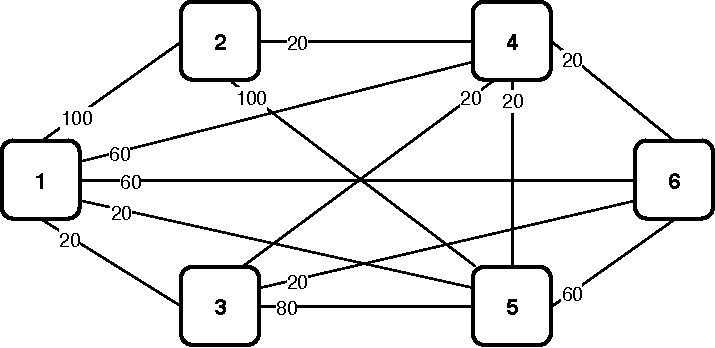
\includegraphics[width=12cm]{sdf/ilp/transparent_survivability/figures/logical_topology_ODU0_high}
\caption{ODU0 logical topology defined by the ODU0 traffic matrix.}
\label{logical2_ODU0_high}
\end{figure}

\begin{figure}[h!]
\centering
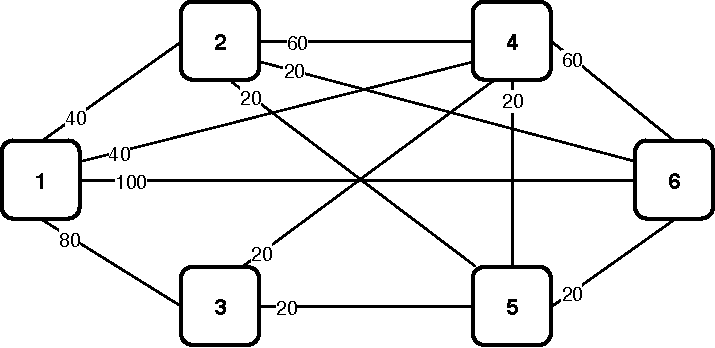
\includegraphics[width=12cm]{sdf/ilp/transparent_survivability/figures/logical_topology_ODU1_high}
\caption{ODU1 logical topology defined by the ODU1 traffic matrix.}
\label{logical2_ODU1_high}
\end{figure}

\begin{figure}[h!]
\centering
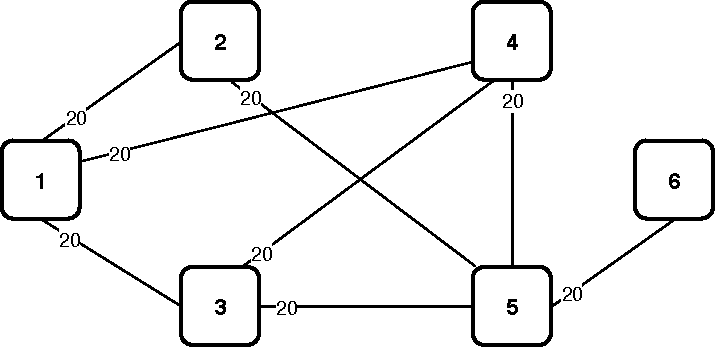
\includegraphics[width=12cm]{sdf/ilp/transparent_survivability/figures/logical_topology_ODU2_high}
\caption{ODU2 logical topology defined by the ODU2 traffic matrix.}
\label{logical2_ODU2_high}
\end{figure}

\begin{figure}[h!]
\centering
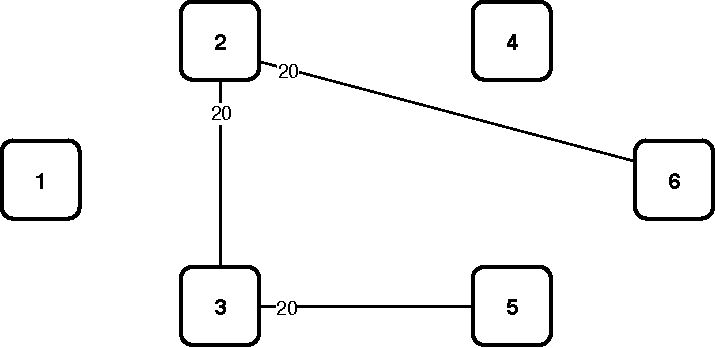
\includegraphics[width=12cm]{sdf/ilp/transparent_survivability/figures/logical_topology_ODU3_high}
\caption{ODU3 logical topology defined by the ODU3 traffic matrix.}
\label{logical2_ODU3_high}
\end{figure}

\begin{figure}[h!]
\centering
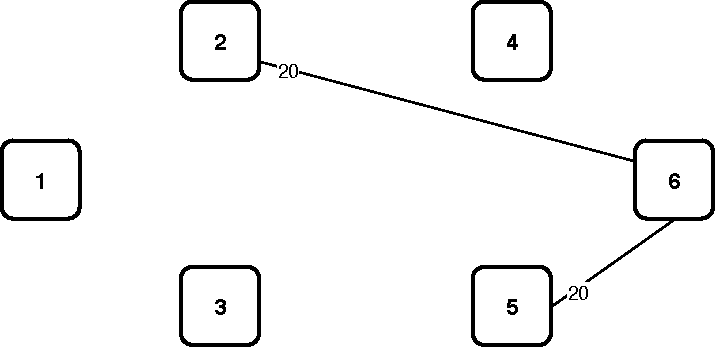
\includegraphics[width=12cm]{sdf/ilp/transparent_survivability/figures/logical_topology_ODU4_high}
\caption{ODU4 logical topology defined by the ODU4 traffic matrix.}
\label{logical2_ODU4_high}
\end{figure}

\begin{figure}[h!]
\centering
\includegraphics[width=12cm]{sdf/ilp/transparent_survivability/figures/physical_topology}
\caption{Physical topology after dimensioning.}
\label{physical2_high}
\end{figure}

\newpage
\begin{figure}[h!]
\centering
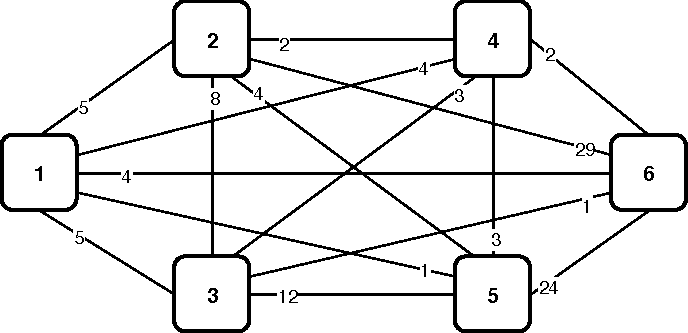
\includegraphics[width=11cm]{sdf/ilp/transparent_survivability/figures/optical_topology_high}
\caption{Optical topology after dimensioning.}
\label{optical2_high}
\end{figure}

In table \ref{link_transp_surv_ref_high} we can see the number of optical channels calculated using \ref{Capex_Link} and \ref{ILPOpaque_CAPEX} and the number of amplifiers for each link calculated using \ref{Capex_amplifiers}.

\begin{table}[h!]
\centering
\begin{tabular}{|| c | c | c ||}
 \hline
 \multicolumn{3}{|| c ||}{Information regarding links} \\
 \hline
 \hline
 Bidirectional Link & Optical Channels & Amplifiers\\
 \hline
 Node 1 <-> Node 2 & 13 & 4 \\
 Node 1 <-> Node 3 & 6 & 6 \\
 Node 2 <-> Node 3 & 15 & 0 \\
 Node 2 <-> Node 4 & 42 & 6 \\
 Node 3 <-> Node 5 & 18 & 8 \\
 Node 4 <-> Node 5 & 3 & 1 \\
 Node 4 <-> Node 6 & 35 & 7 \\
 Node 5 <-> Node 6 & 25 & 3 \\
 \hline
\end{tabular}
\caption{Table with information regarding links for transparent mode.}
\label{link_transp_surv_ref_high}
\end{table}

In table \ref{node_transp_surv_ref_high} we can see the number of line ports and add ports using \ref{OXC_poxc_transparent} the number of long-reach transponders using \ref{EXC_pexc2_transparent} and the number of tributary ports using \ref{EXC_pexc1_transparent}.

\begin{table}[h!]
\centering
\begin{tabular}{|| c | c | c | c | c | c ||}
 \hline
 \multicolumn{6}{|| c ||}{Information regarding nodes} \\
 \hline
 \hline
 \multicolumn{2}{|| c |}{ } & \multicolumn{2}{ c |}{Electrical part} & \multicolumn{2}{ c ||}{Optical part} \\
 \hline
 Node & Resulting Nodal Degree & Tributary Ports & LR Transponders & Add Ports & Line Ports\\
 \hline
 1 & 2 & 580 & 19 & 19 & 19 \\
 2 & 3 & 460 & 48 & 48 & 70 \\
 3 & 3 & 360 & 29 & 29 & 39 \\
 4 & 3 & 400 & 14 & 14 & 80 \\
 5 & 3 & 480 & 44 & 44 & 46 \\
 6 & 2 & 440 & 60 & 60 & 60 \\
\hline
\end{tabular}
\caption{Table with information regarding nodes for transparent mode.}
\label{node_transp_surv_ref_high}
\end{table}

\newpage
Through the information obtained previously on the nodes we can now create tables with detailed information about each node. In each table mentioned below we can see how many ports are connected to a given node and its bit rate (in relation to the line ports and the add ports) and how many ports are assigned to each different bit rate (in relation to the tributary ports).\\

\begin{table}[h!]
\centering
\begin{tabular}{|| c | c | c ||}
 \hline
 \multicolumn{3}{|| c ||}{Detailed description of Node 1} \\
 \hline
 \hline
 Electrical part & Number of total demands & Bit rate \\ \hline
\multirow{3}{*}{580 tributary ports} & 260 & ODU0 \\
 & 260 & ODU1 \\
 & 60 & ODU2 \\
 \hline
  & Node<--Optical Channels-->Node & Bit rate \\
 \hline
 \multirow{5}{*}{19 LR Transponders} & 1  <---- 5 ---->  2 & \multirow{5}{*}{100 Gbits/s} \\
  & 1  <---- 5 ---->  3 & \\
  & 1  <---- 4 ---->  4 & \\
  & 1  <---- 1 ---->  5 & \\
  & 1  <---- 4 ---->  6 & \\
 \hline
 \hline
 Optical part & Node<--Optical Channels-->Node & Bit rate \\
 \hline
 \multirow{5}{*}{19 add ports} & 1  <---- 5 ---->  2 & \multirow{10}{*}{100 Gbits/s} \\
  & 1  <---- 5 ---->  3 & \\
  & 1  <---- 4 ---->  4 & \\
  & 1  <---- 1 ---->  5 & \\
  & 1  <---- 4 ---->  6 & \\ \cline{1-2}
 \multirow{5}{*}{19 line ports} & 1  <---- 5 ---->  2 & \\
  & 1  <---- 5 ---->  3 & \\
  & 1  <---- 4 ---->  4 & \\
  & 1  <---- 1 ---->  5 & \\
  & 1  <---- 4 ---->  6 & \\
\hline
\end{tabular}
\caption{Table with detailed description of node 1. The number of demands is distributed to the various destination nodes, this distribution can be observed in section \ref{high_traffic_scenario}. Regarding the number of line ports when this node is equal to the source, it means that add ports are used, otherwise it means that through ports are used. In this node as we can see there are no through ports.}
\end{table}

\newpage
\begin{table}[h!]
\centering
\begin{tabular}{|| c | c | c ||}
 \hline
 \multicolumn{3}{|| c ||}{Detailed description of Node 2} \\
 \hline
 \hline
 Electrical part & Number of total demands & Bit rate \\ \hline
\multirow{5}{*}{460 tributary ports} & 220 & ODU0 \\
 & 140 & ODU1 \\
 & 40 & ODU2 \\
 & 40 & ODU3 \\
 & 20 & ODU4 \\
 \hline
  & Node<--Optical Channels-->Node & Bit rate \\
 \hline
 \multirow{5}{*}{48 LR Transponders} & 2  <---- 5 ---->  1 & \multirow{5}{*}{100 Gbits/s} \\
  & 2  <---- 8 ---->  3 & \\
  & 2  <---- 2 ---->  4 & \\
  & 2  <---- 4 ---->  5 & \\
  & 2  <---- 29 ---->  6 & \\
 \hline
 \hline
 Optical part & Node<--Optical Channels-->Node & Bit rate \\
 \hline
 \multirow{5}{*}{48 add ports} & 2  <---- 5 ---->  1 & \multirow{13}{*}{100 Gbits/s} \\
  & 2  <---- 8 ---->  3 & \\
  & 2  <---- 2 ---->  4 & \\
  & 2  <---- 4 ---->  5 & \\
  & 2  <---- 29 ---->  6 & \\ \cline{1-2}
 \multirow{8}{*}{70 line ports} & 2  <---- 5 ---->  1 & \\
  & 2  <---- 8 ---->  3 & \\
  & 2  <---- 2 ---->  4 & \\
  & 2  <---- 4 ---->  5 & \\
  & 2  <---- 29 ---->  6 & \\
  & 1  <---- 4 ---->  4 & \\
  & 1  <---- 4 ---->  6 & \\
  & 3  <---- 3 ---->  4 & \\
\hline
\end{tabular}
\caption{Table with detailed description of node 2. The number of demands is distributed to the various destination nodes, this distribution can be observed in section \ref{high_traffic_scenario} . Regarding the number of line ports when this node is equal to the source, it means that add ports are used, otherwise it means that through ports are used. In the latter the number of ports is double the number of optical channels.}
\end{table}

\newpage
\begin{table}[h!]
\centering
\begin{tabular}{|| c | c | c ||}
 \hline
 \multicolumn{3}{|| c ||}{Detailed description of Node 3} \\
 \hline
 \hline
 Electrical part & Number of total demands & Bit rate \\ \hline
\multirow{4}{*}{360 tributary ports} & 140 & ODU0 \\
 & 120 & ODU1\\
 & 60 & ODU2\\
 & 40 & ODU3\\
 \hline
  & Node<--Optical Channels-->Node & Bit rate \\
 \hline
 \multirow{5}{*}{29 LR Transponders} & 3  <---- 5 ---->  1 & \multirow{5}{*}{100 Gbits/s} \\
  & 3  <---- 8 ---->  2 & \\
  & 3  <---- 3 ---->  4 & \\
  & 3  <---- 12 ---->  5 & \\
  & 3  <---- 1 ---->  6 & \\
 \hline
 \hline
 Optical part & Node<--Optical Channels-->Node & Bit rate \\
 \hline
 \multirow{5}{*}{29 add ports} & 3  <---- 5 ---->  1 & \multirow{12}{*}{100 Gbits/s} \\
  & 3  <---- 8 ---->  2 & \\
  & 3  <---- 3 ---->  4 & \\
  & 3  <---- 12 ---->  5 & \\
  & 3  <---- 1 ---->  6 & \\ \cline{1-2}
 \multirow{7}{*}{39 line ports} & 3  <---- 5 ---->  1 & \\
  & 3  <---- 8 ---->  2 & \\
  & 3  <---- 3 ---->  4 & \\
  & 3  <---- 12 ---->  5 & \\
  & 3  <---- 1 ---->  6 & \\
  & 1  <---- 1 ---->  5 & \\
  & 2  <---- 4 ---->  5 & \\ 
\hline
\end{tabular}
\caption{Table with detailed description of node 3. The number of demands is distributed to the various destination nodes, this distribution can be observed in section \ref{high_traffic_scenario} . Regarding the number of line ports when this node is equal to the source, it means that add ports are used, otherwise it means that through ports are used. In the latter the number of ports is double the number of optical channels.}
\end{table}

\newpage
\begin{table}[h!]
\centering
\begin{tabular}{|| c | c | c ||}
 \hline
 \multicolumn{3}{|| c ||}{Detailed description of Node 4} \\
 \hline
 \hline
 Electrical part & Number of total demands & Bit rate \\ \hline
\multirow{3}{*}{400 tributary ports} & 140 & ODU0 \\
 & 200 & ODU1 \\
 & 60 & ODU2 \\
 \hline
  & Node<--Optical Channels-->Node & Bit rate \\
 \hline
 \multirow{5}{*}{14 LR Transponders} & 4  <---- 4 ---->  1 & \multirow{5}{*}{100 Gbits/s} \\
  & 4  <---- 2 ---->  2 & \\
  & 4  <---- 3 ---->  3 & \\
  & 4  <---- 3 ---->  5 & \\
  & 4  <---- 2 ---->  6 & \\
 \hline
 \hline
 Optical part & Node<--Optical Channels-->Node & Bit rate \\
 \hline
 \multirow{5}{*}{14 add ports} & 4  <---- 4 ---->  1 & \multirow{12}{*}{100 Gbits/s} \\
  & 4  <---- 2 ---->  2 & \\
  & 4  <---- 3 ---->  3 & \\
  & 4  <---- 3 ---->  5 & \\
  & 4  <---- 2 ---->  6 & \\ \cline{1-2}
 \multirow{7}{*}{80 line ports} & 4  <---- 4 ---->  1 & \\
  & 4  <---- 2 ---->  2 & \\
  & 4  <---- 3 ---->  3 & \\
  & 4  <---- 3 ---->  5 & \\
  & 4  <---- 2 ---->  6 & \\
  & 1  <---- 4 ---->  6 & \\
  & 2  <---- 29 ---->  6 & \\ 
\hline
\end{tabular}
\caption{Table with detailed description of node 4. The number of demands is distributed to the various destination nodes, this distribution can be observed in section \ref{high_traffic_scenario} . Regarding the number of line ports when this node is equal to the source, it means that add ports are used, otherwise it means that through ports are used. In the latter the number of ports is double the number of optical channels.}
\end{table}

\newpage
\begin{table}[h!]
\centering
\begin{tabular}{|| c | c | c ||}
 \hline
 \multicolumn{3}{|| c ||}{Detailed description of Node 5} \\
 \hline
 \hline
 Electrical part & Number of total demands & Bit rate \\ \hline
\multirow{5}{*}{480 tributary ports} & 280 & ODU0 \\
 & 80 & ODU1 \\
 & 80 & ODU2 \\
 & 20 & ODU3 \\
 & 20 & ODU4 \\
 \hline
  & Node<--Optical Channels-->Node & Bit rate \\
 \hline
 \multirow{5}{*}{44 LR Transponders} & 5  <---- 1 ---->  1 & \multirow{5}{*}{100 Gbits/s} \\
  & 5  <---- 4 ---->  2 & \\
  & 5  <---- 12 ---->  3 & \\
  & 5  <---- 3 ---->  4 & \\
  & 5  <---- 24 ---->  6 & \\
 \hline
 \hline
 Optical part & Node<--Optical Channels-->Node & Bit rate \\
 \hline
 \multirow{5}{*}{44 add ports} & 5  <---- 1 ---->  1 & \multirow{11}{*}{100 Gbits/s} \\
  & 5  <---- 4 ---->  2 & \\
  & 5  <---- 12 ---->  3 & \\
  & 5  <---- 3 ---->  4 & \\
  & 5  <---- 24 ---->  6 & \\ \cline{1-2}
 \multirow{6}{*}{46 line ports} & 5  <---- 1 ---->  1 & \\
  & 5  <---- 4 ---->  2 & \\
  & 5  <---- 12 ---->  3 & \\
  & 5  <---- 3 ---->  4 & \\
  & 5  <---- 24 ---->  6 & \\
  & 3  <---- 1 ---->  6 & \\ 
\hline
\end{tabular}
\caption{Table with detailed description of node 5. The number of demands is distributed to the various destination nodes, this distribution can be observed in section \ref{high_traffic_scenario} . Regarding the number of line ports when this node is equal to the source, it means that add ports are used, otherwise it means that through ports are used. In the latter the number of ports is double the number of optical channels.}
\end{table}

\newpage
\begin{table}[h!]
\centering
\begin{tabular}{|| c | c | c ||}
 \hline
 \multicolumn{3}{|| c ||}{Detailed description of Node 6} \\
 \hline
 \hline
 Electrical part & Number of total demands & Bit rate \\ \hline
\multirow{5}{*}{440 tributary ports} & 160 & ODU0 \\
 & 200 & ODU1 \\
 & 20 & ODU2 \\
 & 20 & ODU3 \\
 & 40 & ODU4 \\
 \hline
  & Node<--Optical Channels-->Node & Bit rate \\
 \hline
 \multirow{5}{*}{60 LR Transponders} & 6  <---- 4 ---->  1 & \multirow{5}{*}{100 Gbits/s} \\
  & 6  <---- 29 ---->  2 & \\
  & 6  <---- 1 ---->  3 & \\
  & 6  <---- 2 ---->  4 & \\
  & 6  <---- 24 ---->  5 & \\
 \hline
 \hline
 Optical part & Node<--Optical Channels-->Node & Bit rate \\
 \hline
 \multirow{5}{*}{60 add ports} & 6  <---- 4 ---->  1 & \multirow{10}{*}{100 Gbits/s} \\
  & 6  <---- 29 ---->  2 & \\
  & 6  <---- 1 ---->  3 & \\
  & 6  <---- 2 ---->  4 & \\
  & 6  <---- 24 ---->  5 & \\ \cline{1-2}
 \multirow{5}{*}{60 line ports} & 6  <---- 4 ---->  1 & \\
  & 6  <---- 29 ---->  2 & \\
  & 6  <---- 1 ---->  3 & \\
  & 6  <---- 2 ---->  4 & \\
  & 6  <---- 24 ---->  5 & \\
\hline
\end{tabular}
\caption{Table with detailed description of node 6. The number of demands is distributed to the various destination nodes, this distribution can be observed in section \ref{high_traffic_scenario}. Regarding the number of line ports when this node is equal to the source, it means that add ports are used, otherwise it means that through ports are used. In this node as we can see there are no through ports.}
\end{table}

\vspace{17pt}
Now, in next page, let's focus on the routing information in table \ref{path_transp_surv_ref_high}. These paths are bidirectional so the path from one node to another is the same path in the opposite direction.\\
\newpage
\begin{table}[h!]
\centering
\begin{tabular}{|| c | c | c ||}
 \hline
 \multicolumn{3}{|| c ||}{Routing} \\
 \hline
 \hline
 o & d & Links \\
 \hline
 1 & 2 & \{(1,2)\} \\ \hline
 1 & 3 & \{(1,3)\} \\ \hline
 1 & 4 & \{(1,2),(2,4)\}\\ \hline
 1 & 5 & \{(1,3),(3,5)\}\\ \hline
 1 & 6 & \{(1,2),(2,4),(4,6)\}\\ \hline
 2 & 3 & \{(2,3)\}\\ \hline
 2 & 4 & \{(2,4)\}\\ \hline
 2 & 5 & \{(2,3),(3,5)\}\\ \hline
 2 & 6 & \{(2,4),(4,6)\}\\ \hline
 3 & 4 & \{(3,2),(2,4)\}\\ \hline
 3 & 5 & \{(3,5)\}\\ \hline
 3 & 6 & \{(3,5),(5,6)\}\\ \hline
 4 & 5 & \{(4,5)\}\\ \hline
 4 & 6 & \{(4,6)\}\\ \hline
 5 & 6 & \{(5,6)\}\\
 \hline
\end{tabular}
\caption{Table with description of routing}
\label{path_transp_surv_ref_high}
\end{table}

Finally and most importantly through table \ref{scripttransp_surv_ref_high} we can see the CAPEX result for this model. This value is obtained using equation \ref{ILPOpaque_CAPEX} and all of the constraints mentioned above. In table \ref{formulas_transp} mentioned in previous scenario we can see how all the values were calculated.

\begin{table}[h!]
\centering
\begin{tabular}{|| c | c | c | c | c | c | c ||}
 \hline
 \multicolumn{7}{|| c ||}{CAPEX of the Network} \\
 \hline
 \hline
 \multicolumn{3}{|| c |}{ } & Quantity & Unit Price & Cost & Total \\
 \hline
 \multirow{3}{*}{Link Cost} & \multicolumn{2}{ c |}{OLTs} & 16 & 15 000 \euro & 240 000 \euro & \multirow{3}{*}{157 520 000 \euro} \\ \cline{2-6}
 & \multicolumn{2}{ c |}{100 Gbits/s Transceivers} & 314 & 5 000 \euro/Gbit/s & 157 000 000 \euro & \\ \cline{2-6}
 & \multicolumn{2}{ c |}{Amplifiers} & 70 & 4 000 \euro & 280 000 \euro & \\
 \hline
 \multirow{10}{*}{Node Cost} & \multirow{7}{*}{Electrical} & EXCs & 6 & 10 000 \euro & 60 000 \euro & \multirow{10}{*}{22 951 800 \euro} \\ \cline{3-6}
 & & ODU0 Ports & 1 200 & 10 \euro/port & 12 000 \euro & \\ \cline{3-6}
 & & ODU1 Ports & 1 000 & 15 \euro/port & 15 000 \euro & \\ \cline{3-6}
 & & ODU2 Ports & 320 & 30 \euro/port & 9 600 \euro & \\ \cline{3-6}
 & & ODU3 Ports & 120 & 60 \euro/port & 7 200 \euro & \\ \cline{3-6}
 & & ODU4 Ports & 80 & 100 \euro/port & 8 000 \euro & \\ \cline{3-6}
 & &Transponders& 214 & 100 000 \euro/port & 21 400 000 \euro & \\ \cline{2-6}
 & \multirow{3}{*}{Optical} & OXCs & 6 & 20 000 \euro & 120 000 \euro & \\ \cline{3-6}
 & & Line Ports & 314 & 2 500 \euro/port & 785 000 \euro & \\ \cline{3-6}
 & & Add Ports & 214 & 2 500 \euro/port & 535 000 \euro & \\
 \hline
 \multicolumn{6}{|| c |}{Total Network Cost} & 180 471 800 \euro \\
\hline
\end{tabular}
\caption{Table with detailed description of CAPEX for this scenario.}
\label{scripttransp_surv_ref_high}
\end{table}

\newpage
\subsubsection{Conclusions}

Once we have obtained the results for all the scenarios we will now draw some conclusions about these results. For a better analysis of the results will be created the table \ref{table_comparative_transp_surv} with the number of line ports and add ports of the optical part, the tributary ports, the transponders and transceivers because they are important values for the cost of CAPEX, the cost of links, the cost of nodes and finally the cost of CAPEX.\\

\begin{table}[h!]
\centering
\begin{tabular}{| c | c | c | c |}
 \hline
  & Low Traffic & Medium Traffic  & High Traffic \\
 \hline\hline
 Traffic (Gbit/s) & 500 & 5 000 & 10 000 \\ \hline
 Number of Add ports & 34 & 114 & 214 \\ \hline
 Number of Line ports & 52 & 168 & 314 \\ \hline
 Number of Tributary ports & 136 & 1 360 & 2 720 \\ \hline
 Number of Transceivers & 52 & 168 & 314 \\ \hline
 Number of Transponders & 34 & 114 & 214 \\ \hline
 Link Cost & 26 520 000 \euro & 84 520 000 \euro & 157 520 000 \euro \\ \hline
 Node Cost & 3 797 590 \euro & 12 310 900 \euro & 22 951 800 \euro \\ \hline
 CAPEX & \textbf{30 317 590 \euro} & \textbf{96 830 900 \euro} & \textbf{180 471 800 \euro} \\ \hline
 CAPEX/Gbit/s & \textbf{60 635.18 \euro/Gbit/s} & \textbf{19 366.18 \euro/Gbit/s} & \textbf{18 047.68 \euro/Gbit/s}\\
 \hline
\end{tabular}
\caption{Table with the various CAPEX values obtained in the different traffic scenarios.}
\label{table_comparative_transp_surv}
\end{table}

Looking at the previous table we can make some comparisons between the several scenarios:

\begin{itemize}
    \item Comparing the low traffic scenario with the others, we can see that, despite having an increase of factor ten (average scenario) and factor twenty (high scenario), the same increase does not occur in the final cost (it is lower). This happens because the number of transceivers is smaller than expected (an average scenario of 520 would be expected and a high scenario would be expected in 1040);
    \item Comparing the medium traffic scenario with the high traffic scenario, we can see that the factor increase is double and in the final cost this factor is very close but still lower. Again, this happens because the number of transceivers is smaller, but very close to what was expected (the high scenario would be expected at 336);
    \item Comparing the cost with the traffic, we see that, for the low traffic scenario, the cost per traffic is very high in relation to the other two. We can conclude that a low traffic scenario becomes more expensive than a high traffic scenario.
\end{itemize}


\vspace{13pt}
\subsubsection{Opens Issues}

The creation of this model for any scenario, started with some considerations and some open issues being:

\begin{itemize}
  \item Allow blocking.
  \subitem The presented model assume that the solution is possible or impossible, does not support a partial solution where some demands are not routed (are blocked).
  \item Allow multiple transmission system.
  \subitem The presented model for each link only supports one transmission system.
\end{itemize}


\clearpage

\subsection{Transparent with 1+1 Protection}\label{ILP_Transp_Protection}
\begin{tcolorbox}	
\begin{tabular}{p{2.75cm} p{0.2cm} p{10.5cm}} 	
\textbf{Student Name}  &:& Tiago Esteves    (October 03, 2017 - )\\
\textbf{Goal}          &:& Implement the ILP model for the transparent transport mode with 1 plus 1 protection.
\end{tabular}
\end{tcolorbox}
\vspace{11pt}

Here, in this case, we must take into account table \ref{description_transp}, previously mentioned, in order to better understand the objective function.\\

Before carrying out the description of the objective function we must take into account the following particularity of this mode of transport:
\begin{itemize}
  \item $N_{OXC,n}$ = 1, \quad $\forall$ n that process traffic
  \item $N_{EXC,n}$ = 1, \quad $\forall$ n that process traffic
\end{itemize}

\vspace{11pt}
The objective function of following the ILP is a minimization of the CAPEX through the equation \ref{Capex} where in this case for the cost of nodes we have in consideration the electric cost \ref{Capex_Node_EXC} and the optical cost \ref{Capex_Node_OXC}.
In this case the value of $P_{exc,c,n}$ is obtained by equation \ref{EXC_pexc1_transparentp} for short-reach and by the equation \ref{EXC_pexc2_transparentp} for long-reach and the value of $P_{oxc,n}$ is obtained by equation \ref{OXC_poxc_transparentp}.\\

The equation \ref{EXC_pexc1_transparentp} refers to the number of sort-reach ports of the electrical switch with bit-rate $c$ in node $n$, $P_{exc,c,n}$, i.e. the number of tributary ports with bit-rate $c$ in node $n$ which can be calculated as

\begin{equation}
P_{exc,c,n} = \sum_{d=1}^{N} D_{nd,c}
\label{EXC_pexc1_transparentp}
\end{equation}

\vspace{11pt}
\noindent
where $D_{nd,c}$ are the client demands between nodes $n$ and $d$ with bit rate $c$.\\

In this case there is the following particularity:

\begin{itemize}
  \item When $n$=$d$ the value of client demands is always zero, i.e, $D_{nn,c}=0$
\end{itemize}

\vspace{11pt}
As previously mentioned, the equation \ref{EXC_pexc2_transparentp} refers to the number of long-reach ports of the electrical switch with bit-rate -1 in node n, $P_{exc,-1,n}$, i.e. the number of add ports of node n which can be calculated as

\begin{equation}
P_{exc,-1,n} = \sum_{j=1}^{N} \lambda_{nj}
\label{EXC_pexc2_transparentp}
\end{equation}

\vspace{11pt}
\noindent
where $\lambda_{nj}$ is the number of optical channels between node $n$ and node $j$.\\

The equation \ref{OXC_poxc_transparentp} refers to the number of ports in optical switch in node n, $P_{oxc,n}$, i.e. the number of line ports and the number of adding ports of node n which can be calculated as

\begin{equation}
P_{oxc,n} = \sum_{j=1}^{N} f_{nj}^{od} + \sum_{j=1}^{N} \lambda_{nj}
\label{OXC_poxc_transparentp}
\end{equation}

\vspace{11pt}
\noindent
where $f_{nj}^{od}$ refers to the number of line ports for all demand pairs (od) and $\lambda_{nj}$ refers to the number of add ports.\\

The objective function, to be minimized, is the expression \ref{ILPOpaque_CAPEX}, i.e.,
\begin{equation*}
  minimize \qquad \Big\{ \quad C_C \quad \Big\}
\end{equation*}

$subject$ $to$
\begin{equation}
\sum_{c\in C} B\left(c\right) D_{odc} \leq \tau \lambda_{od} \qquad \qquad \qquad \qquad \qquad \qquad \qquad \qquad \qquad \qquad
\forall(o,d) : o < d
\label{ILPTransp0}
\end{equation}
\noindent
This restriction is considered grooming constraint and for this model the grooming can be done before routing since the traffic is aggregated just for demands between the same nodes, thus not depending on the routes. The variable  $\tau$ is always 100 Gbits/s.

\begin{equation}
\sum_{j\textbackslash \{o\}} f_{ij}^{od} = \lambda_{od} \qquad \qquad \qquad \qquad \qquad \qquad \qquad \qquad \qquad
\forall(o,d) : o < d, \forall i: i = o
\label{ILPTransp1}
\end{equation}
\noindent
This constraint are equal to the constraint \ref{ILPOpaque1_CAPEX} assuming that Z variable has the value of number of optical channels between this demand for all bidirectional links.

\begin{equation}
\sum_{j\textbackslash \{o\}} f_{ij}^{od} = \sum_{j\textbackslash \{d\}} f_{ji}^{od} \qquad \qquad \qquad \qquad \qquad \qquad \qquad \qquad
\forall(o,d) : o < d, \forall i: i \neq o,d
\label{ILPTransp2}
\end{equation}
\noindent
This constraint are equal to the constraint \ref{ILPOpaque2_CAPEX}.

\begin{equation}
\sum_{j\textbackslash \{d\}} f_{ji}^{od} = \lambda_{od}  \qquad \qquad \qquad \qquad \qquad \qquad \qquad \qquad \qquad
\forall(o,d) : o < d, \forall i: i = d
\label{ILPTransp3}
\end{equation}
\noindent
This constraint are equal to the constraint \ref{ILPOpaque3_CAPEX} assuming that Z variable has the value of number of optical channels between this demand for all bidirectional links.
\newpage
\begin{equation}
\sum_{j\textbackslash \{o\}} fp_{ij}^{od} = \lambda_{od} \qquad \qquad \qquad \qquad \qquad \qquad \qquad \qquad \qquad
\forall(o,d) : o < d, \forall i: i = o
\label{ILPTransp1p}
\end{equation}
\noindent
This are the protection flow conservation constraints and ensure that, for each $(o,d)$ pair, we route the number of optical channels units of flow from node $o$ to node $d$, the source node sends the number of optical channels units of flow.

\begin{equation}
\sum_{j\textbackslash \{o\}} fp_{ij}^{od} = \sum_{j\textbackslash \{d\}} fp_{ji}^{od} \qquad \qquad \qquad \qquad \qquad \qquad \qquad
\forall(o,d) : o < d, \forall i: i \neq o,d
\label{ILPTransp2p}
\end{equation}
\noindent
This constraint ensure that the remaining nodes, being neither origin or destination, the receive flow have to be send.

\begin{equation}
\sum_{j\textbackslash \{d\}} fp_{ji}^{od} = \lambda_{od} \qquad \qquad \qquad \qquad \qquad \qquad \qquad \qquad \qquad
\forall(o,d) : o < d, \forall i: i = d
\label{ILPTransp3p}
\end{equation}
\noindent
This are the usual flow conservation constraints and ensure that, for each $(o,d)$ pair, we route the number of optical channels units of flow from node $o$ to node $d$, the destination node has to receive those numbers of optical channels units of flow.

\begin{equation}
\sum_{o=1} \sum_{d=o+1} \left(f_{ij}^{od}  + fp_{ij}^{od}\right) \leq \lambda_{od}  \qquad \qquad \qquad \qquad \qquad \qquad \qquad \qquad \qquad
\forall (o,d), (i,j)
\label{ILPTransp4p}
\end{equation}
\noindent
This constraint assures us that the variable $f_{ij}^{od}$ (working flow) and $fp_{ij}^{od}$ (protection flow) are different.

\begin{equation}
\sum_{o=1} \sum_{d=o+1} \left(f_{ij}^{od} + f_{ji}^{od} + fp_{ij}^{od} + fp_{ji}^{od}\right) \leq K_{ij} G_{ij} L_{ij} \qquad \qquad \qquad \qquad
\forall(i,j) : i < j
\label{ILPTransp4}
\end{equation}
\noindent
This restriction answers capacity constraint problem. Then, total flows must be less or equal to the capacity of network links. For any situation the maximum number of optical channels supported by each transmission system is 100, i.e., $K_{ij}$ = 100.

\begin{equation}
f_{ij}^{od} , f_{ji}^{od} , fp_{ij}^{od} , fp_{ji}^{od} , \lambda_{od} \in \mathbb{N}   \qquad \qquad \qquad \qquad \qquad
\forall(i,j) : i < j, \forall(o,d) : o < d
\label{ILPTransp5}
\end{equation}
\noindent
This constraint define the total number of flows and the number of optical channels must be a counting number.

\begin{equation}
L_{i,j} \in \{0,1\} \qquad \qquad \qquad \qquad \qquad \qquad \qquad \qquad \qquad \qquad \qquad \qquad \qquad \qquad
\forall(i,j)
\label{ILPTranspL1}
\end{equation}
\noindent
Last constraint refers to the use of the link where this variable can be zero if it is not being used or one if is being used.\\


\subsubsection{Result description}

To perform the calculations using the implementation of the models described previously it is necessary to use a mathematical software tool. For this we will use MATLAB which is ideal for dealing with linear programming problems and can call the LPsolve through an external interface. We already have all the necessary to obtain the CAPEX value for the reference network \ref{Reference_Network_Topology}. As described in the subsection of network traffic \ref{Reference_Network_Traffic}, we have three values of network traffic (low, medium and high traffic) so we have to obtain three different CAPEX. The value of the CAPEX of the network will be calculated based on the costs of the equipment present in the table \ref{table_cost_ilp}.\\

\vspace{17pt}
\textbf{Low Traffic Scenario:}\\

In this scenario we have to take into account the traffic calculated in \ref{low_scenario}. In a first phase we will show the various existing topologies of the network. The first are the allowed topologies, physical and optical topology, the second are the logical topology for all ODUs and finally the resulting physical and optical topology.\\

\begin{figure}[h!]
\centering
\includegraphics[width=13cm]{sdf/ilp/transparent_protection/figures/allowed_physical_topology}
\caption{Allowed physical topology. The allowed physical topology is defined by the duct and sites in the field. It is assumed that each duct supports up to 1 bidirectional transmission system and each site supports up to 1 node.}
\label{allowed2_physical_protectionlow}
\end{figure}
\newpage
\begin{figure}[h!]
\centering
\includegraphics[width=11cm]{sdf/ilp/transparent_protection/figures/allowed_optical_topology}
\caption{Allowed optical topology. The allowed optical topology is defined by the transport mode (transparent transport mode in this case). It is assumed that each connections between demands supports up to 100 lightpaths.}
\label{allowed2_optical_protectionlow}
\end{figure}

\begin{figure}[h!]
\centering
\includegraphics[width=11cm]{sdf/ilp/transparent_protection/figures/logical_topology_ODU0_low}
\caption{ODU0 logical topology defined by the ODU0 traffic matrix.}
\label{logical2_ODU0_protectionlow}
\end{figure}

\begin{figure}[h!]
\centering
\includegraphics[width=11cm]{sdf/ilp/transparent_protection/figures/logical_topology_ODU1_low}
\caption{ODU1 logical topology defined by the ODU1 traffic matrix.}
\label{logical2_ODU1_protectionlow}
\end{figure}
\newpage
\begin{figure}[h!]
\centering
\includegraphics[width=12cm]{sdf/ilp/transparent_protection/figures/logical_topology_ODU2_low}
\caption{ODU2 logical topology defined by the ODU2 traffic matrix.}
\label{logical2_ODU2_protectionlow}
\end{figure}

\begin{figure}[h!]
\centering
\includegraphics[width=12cm]{sdf/ilp/transparent_protection/figures/logical_topology_ODU3_low}
\caption{ODU3 logical topology defined by the ODU3 traffic matrix.}
\label{logical2_ODU3_protectionlow}
\end{figure}

\begin{figure}[h!]
\centering
\includegraphics[width=12cm]{sdf/ilp/transparent_protection/figures/logical_topology_ODU4_low}
\caption{ODU4 logical topology defined by the ODU4 traffic matrix.}
\label{logical2_ODU4_protectionlow}
\end{figure}
\newpage
\begin{figure}[h!]
\centering
\includegraphics[width=13cm]{sdf/ilp/transparent_protection/figures/physical_topology}
\caption{Physical topology after dimensioning.}
\label{physical2_protectionlow}
\end{figure}

\vspace{17pt}
\begin{figure}[h!]
\centering
\includegraphics[width=13cm]{sdf/ilp/transparent_protection/figures/optical_topology_low}
\caption{Optical topology after dimensioning.}
\label{optical2_protectionlow}
\end{figure}

\vspace{17pt}
In table \ref{link_transp_protec_ref_low} we can see the number of optical channels calculated using \ref{Capex_Link} and \ref{ILPOpaque_CAPEX} and the number of amplifiers for each link calculated using \ref{Capex_amplifiers}.\\

In table \ref{node_transp_protec_ref_low} we can see the resulting nodal degree at the physical layer, calculated based on the number of connections that the node in question performs, the number of line ports and the number of add ports for the optical part calculated using \ref{OXC_poxc_transparentp} the number of long-reach transponders calculated using \ref{EXC_pexc2_transparentp} and the number of tributary ports calculated using \ref{EXC_pexc1_transparentp} for each node.\\

\newpage
\begin{table}[h!]
\centering
\begin{tabular}{|| c | c | c ||}
 \hline
 \multicolumn{3}{|| c ||}{Information regarding links} \\
 \hline
 \hline
 Bidirectional Link & Optical Channels & Amplifiers\\
 \hline
 Node 1 <-> Node 2 & 6 & 4 \\
 Node 1 <-> Node 3 & 6 & 6 \\
 Node 2 <-> Node 3 & 10 & 0 \\
 Node 2 <-> Node 4 & 10 & 6 \\
 Node 3 <-> Node 5 & 10 & 8 \\
 Node 4 <-> Node 5 & 10 & 1 \\
 Node 4 <-> Node 6 & 8 & 7 \\
 Node 5 <-> Node 6 & 8 & 3 \\
 \hline
\end{tabular}
\caption{Table with information regarding links for transparent mode with 1+1 protection.}
\label{link_transp_protec_ref_low}
\end{table}

\vspace{15pt}
\begin{table}[h!]
\centering
\begin{tabular}{|| c | c | c | c | c | c ||}
 \hline
 \multicolumn{6}{|| c ||}{Information regarding nodes} \\
 \hline
 \hline
 \multicolumn{2}{|| c |}{ } & \multicolumn{2}{ c |}{Electrical part} & \multicolumn{2}{ c ||}{Optical part} \\
 \hline
 Node & Resulting Nodal Degree & Tributary Ports & LR Transponders & Add Ports & Line Ports\\
 \hline
 1 & 2 & 29 & 5 & 5 & 12 \\
 2 & 3 & 23 & 6 & 6 & 26 \\
 3 & 3 & 18 & 5 & 5 & 26 \\
 4 & 3 & 20 & 5 & 5 & 28 \\
 5 & 3 & 24 & 6 & 6 & 28 \\
 6 & 2 & 22 & 7 & 7 & 16 \\
\hline
\end{tabular}
\caption{Table with information regarding nodes for transparent mode with 1+1 protection.}
\label{node_transp_protec_ref_low}
\end{table}

\vspace{15pt}
Through the information obtained previously on the nodes we can now create tables with detailed information about each node. In each table mentioned below we can see how many ports are connected to a given node and its bit rate (in relation to the line ports and the add ports) and how many ports are assigned to each different bit rate (in relation to the tributary ports).\\
\newpage
\begin{table}[h!]
\centering
\begin{tabular}{|| c | c | c ||}
 \hline
 \multicolumn{3}{|| c ||}{Detailed description of Node 1} \\
 \hline
 \hline
 Electrical part & Number of tributary ports & Bit rate \\ \hline
\multirow{3}{*}{29 tributary ports} & 13 & ODU0 \\
 & 13 & ODU1 \\
 & 3 & ODU2 \\
 \hline
  & Node<--Optical Channels-->Node & Bit rate \\
 \hline
 \multirow{5}{*}{5 LR Transponders} & 1  <---- 1 ---->  2 & \multirow{5}{*}{100 Gbits/s} \\
  & 1  <---- 1 ---->  3 & \\
  & 1  <---- 1 ---->  4 & \\
  & 1  <---- 1 ---->  5 & \\
  & 1  <---- 1 ---->  6 & \\
 \hline
 \hline
 Optical part & Node<--Optical Channels-->Node & Bit rate \\
 \hline
 \multirow{5}{*}{5 add ports} & 1  <---- 1 ---->  2 & \multirow{11}{*}{100 Gbits/s} \\
  & 1  <---- 1 ---->  3 & \\
  & 1  <---- 1 ---->  4 & \\
  & 1  <---- 1 ---->  5 & \\
  & 1  <---- 1 ---->  6 & \\ \cline{1-2}
 \multirow{6}{*}{12 line ports} & 1  <---- 1 ---->  2 & \\
  & 1  <---- 1 ---->  3 & \\
  & 1  <---- 1 ---->  4 & \\
  & 1  <---- 1 ---->  5 & \\
  & 1  <---- 1 ---->  6 & \\
  & 2  <---- 1 ---->  3 & \\
\hline
\end{tabular}
\caption{Table with detailed description of node 1. The number of demands is distributed to the various destination nodes, this distribution can be observed in section \ref{low_scenario}. Regarding the number of line ports when this node is equal to the source, it means that add ports are used, otherwise it means that through ports are used. In both cases the number of ports is double the number of optical channels.}
\end{table}

\newpage
\begin{table}[h!]
\centering
\begin{tabular}{|| c | c | c ||}
 \hline
 \multicolumn{3}{|| c ||}{Detailed description of Node 2} \\
 \hline
 \hline
 Electrical part & Number of tributary ports & Bit rate \\ \hline
\multirow{5}{*}{23 tributary ports} & 11 & ODU0 \\
 & 7 & ODU1 \\
 & 2 & ODU2 \\
 & 2 & ODU3 \\
 & 1 & ODU4 \\
 \hline
  & Node<--Optical Channels-->Node & Bit rate \\
 \hline
 \multirow{5}{*}{6 LR Transponders} & 2  <---- 1 ---->  1 & \multirow{5}{*}{100 Gbits/s}\\
  & 2  <---- 1 ---->  3 & \\
  & 2  <---- 1 ---->  4 & \\
  & 2  <---- 1 ---->  5 & \\
  & 2  <---- 2 ---->  6 & \\
 \hline
 \hline
 Optical part & Node<--Optical Channels-->Node & Bit rate \\
 \hline
 \multirow{5}{*}{6 add ports} & 2  <---- 1 ---->  1 & \multirow{17}{*}{100 Gbits/s} \\
  & 2  <---- 1 ---->  3 & \\
  & 2  <---- 1 ---->  4 & \\
  & 2  <---- 1 ---->  5 & \\
  & 2  <---- 2 ---->  6 & \\ \cline{1-2}
 \multirow{12}{*}{26 line ports} & 2  <---- 1 ---->  1 & \\
  & 2  <---- 1 ---->  3 & \\
  & 2  <---- 1 ---->  4 & \\
  & 2  <---- 1 ---->  5 & \\
  & 2  <---- 2 ---->  6 & \\
  & 1  <---- 1 ---->  3 & \\
  & 1  <---- 1 ---->  4 & \\
  & 1  <---- 1 ---->  5 & \\
  & 1  <---- 1 ---->  6 & \\
  & 3  <---- 1 ---->  4 & \\
  & 3  <---- 1 ---->  5 & \\
  & 3  <---- 1 ---->  6 & \\
\hline
\end{tabular}
\caption{Table with detailed description of node 2. The number of demands is distributed to the various destination nodes, this distribution can be observed in section \ref{low_scenario}. Regarding the number of line ports when this node is equal to the source, it means that add ports are used, otherwise it means that through ports are used. In both cases the number of ports is double the number of optical channels.}
\end{table}

\newpage
\begin{table}[h!]
\centering
\begin{tabular}{|| c | c | c ||}
 \hline
 \multicolumn{3}{|| c ||}{Detailed description of Node 3} \\
 \hline
 \hline
 Electrical part & Number of tributary ports & Bit rate \\ \hline
\multirow{4}{*}{18 tributary ports} & 7 & ODU0 \\
 & 6 & ODU1\\
 & 3 & ODU2\\
 & 2 & ODU3\\
 \hline
  & Node<--Optical Channels-->Node & Bit rate \\
 \hline
 \multirow{5}{*}{5 LR Transponders} & 3  <---- 1 ---->  1 & \multirow{5}{*}{100 Gbits/s} \\
  & 3  <---- 1 ---->  2 & \\
  & 3  <---- 1 ---->  4 & \\
  & 3  <---- 1 ---->  5 & \\
  & 3  <---- 1 ---->  6 & \\
 \hline
 \hline
 Optical part & Node<--Optical Channels-->Node & Bit rate \\
 \hline
 \multirow{5}{*}{5 add ports} & 3  <---- 1 ---->  1 & \multirow{17}{*}{100 Gbits/s} \\
  & 3  <---- 1 ---->  2 & \\
  & 3  <---- 1 ---->  4 & \\
  & 3  <---- 1 ---->  5 & \\
  & 3  <---- 1 ---->  6 & \\ \cline{1-2}
 \multirow{12}{*}{26 line ports} & 3  <---- 1 ---->  1 & \\
  & 3  <---- 1 ---->  2 & \\
  & 3  <---- 1 ---->  4 & \\
  & 3  <---- 1 ---->  5 & \\
  & 3  <---- 1 ---->  6 & \\
  & 1  <---- 1 ---->  2 & \\
  & 1  <---- 1 ---->  4 & \\
  & 1  <---- 1 ---->  5 & \\
  & 1  <---- 1 ---->  6 & \\
  & 2  <---- 1 ---->  4 & \\
  & 2  <---- 1 ---->  5 & \\
  & 2  <---- 2 ---->  6 & \\
\hline
\end{tabular}
\caption{Table with detailed description of node 3. The number of demands is distributed to the various destination nodes, this distribution can be observed in section \ref{low_scenario}. Regarding the number of line ports when this node is equal to the source, it means that add ports are used, otherwise it means that through ports are used. In both cases the number of ports is double the number of optical channels.}
\end{table}

\newpage
\begin{table}[h!]
\centering
\begin{tabular}{|| c | c | c ||}
 \hline
 \multicolumn{3}{|| c ||}{Detailed description of Node 4} \\
 \hline
 \hline
 Electrical part & Number of tributary ports & Bit rate \\ \hline
\multirow{3}{*}{20 tributary ports} & 7 & ODU0 \\
 & 10 & ODU1 \\
 & 3 & ODU2 \\
 \hline
  & Node<--Optical Channels-->Node & Bit rate \\
 \hline
 \multirow{5}{*}{5 LR Transponders} & 4  <---- 1 ---->  1 & \multirow{5}{*}{100 Gbits/s} \\
  & 4  <---- 1 ---->  2 & \\
  & 4  <---- 1 ---->  3 & \\
  & 4  <---- 1 ---->  5 & \\
  & 4  <---- 1 ---->  6 & \\
 \hline
 \hline
 Optical part & Node<--Optical Channels-->Node & Bit rate \\
 \hline
 \multirow{5}{*}{5 add ports} & 4  <---- 1 ---->  1 & \multirow{17}{*}{100 Gbits/s} \\
  & 4  <---- 1 ---->  2 & \\
  & 4  <---- 1 ---->  3 & \\
  & 4  <---- 1 ---->  5 & \\
  & 4  <---- 1 ---->  6 & \\ \cline{1-2}
 \multirow{12}{*}{28 line ports} & 4  <---- 1 ---->  1 & \\
  & 4  <---- 1 ---->  2 & \\
  & 4  <---- 1 ---->  3 & \\
  & 4  <---- 1 ---->  5 & \\
  & 4  <---- 1 ---->  6 & \\
  & 1  <---- 1 ---->  5 & \\
  & 1  <---- 1 ---->  6 & \\
  & 2  <---- 1 ---->  5 & \\
  & 2  <---- 2 ---->  6 & \\
  & 3  <---- 1 ---->  5 & \\
  & 3  <---- 1 ---->  6 & \\
  & 5  <---- 2 ---->  6 & \\
\hline
\end{tabular}
\caption{Table with detailed description of node 4. The number of demands is distributed to the various destination nodes, this distribution can be observed in section \ref{low_scenario}. Regarding the number of line ports when this node is equal to the source, it means that add ports are used, otherwise it means that through ports are used. In both cases the number of ports is double the number of optical channels.}
\end{table}

\newpage
\begin{table}[h!]
\centering
\begin{tabular}{|| c | c | c ||}
 \hline
 \multicolumn{3}{|| c ||}{Detailed description of Node 5} \\
 \hline
 \hline
 Electrical part & Number of tributary ports & Bit rate \\ \hline
\multirow{5}{*}{24 tributary ports} & 14 & ODU0 \\
 & 4 & ODU1 \\
 & 4 & ODU2 \\
 & 1 & ODU3 \\
 & 1 & ODU4 \\
 \hline
  & Node<--Optical Channels-->Node & Bit rate \\
 \hline
 \multirow{5}{*}{6 LR Transponders} & 5  <---- 1 ---->  1 & \multirow{5}{*}{100 Gbits/s} \\
  & 5  <---- 1 ---->  2 & \\
  & 5  <---- 1 ---->  3 & \\
  & 5  <---- 1 ---->  4 & \\
  & 5  <---- 2 ---->  6 & \\
 \hline
 \hline
 Optical part & Node<--Optical Channels-->Node & Bit rate \\
 \hline
 \multirow{5}{*}{6 add ports} & 5  <---- 1 ---->  1 & \multirow{17}{*}{100 Gbits/s} \\
  & 5  <---- 1 ---->  2 & \\
  & 5  <---- 1 ---->  3 & \\
  & 5  <---- 1 ---->  4 & \\
  & 5  <---- 2 ---->  6 & \\ \cline{1-2}
 \multirow{12}{*}{28 line ports} & 5  <---- 1 ---->  1 & \\
  & 5  <---- 1 ---->  2 & \\
  & 5  <---- 1 ---->  3 & \\
  & 5  <---- 1 ---->  4 & \\
  & 5  <---- 2 ---->  6 & \\
  & 1  <---- 1 ---->  4 & \\
  & 1  <---- 1 ---->  6 & \\
  & 2  <---- 1 ---->  4 & \\
  & 2  <---- 2 ---->  6 & \\
  & 3  <---- 1 ---->  4 & \\
  & 3  <---- 1 ---->  6 & \\
  & 4  <---- 1 ---->  6 & \\
\hline
\end{tabular}
\caption{Table with detailed description of node 5. The number of demands is distributed to the various destination nodes, this distribution can be observed in section \ref{low_scenario}. Regarding the number of line ports when this node is equal to the source, it means that add ports are used, otherwise it means that through ports are used. In both cases the number of ports is double the number of optical channels.}
\end{table}

\newpage
\begin{table}[h!]
\centering
\begin{tabular}{|| c | c | c ||}
 \hline
 \multicolumn{3}{|| c ||}{Detailed description of Node 6} \\
 \hline
 \hline
 Electrical part & Number of tributary ports & Bit rate \\ \hline
\multirow{5}{*}{22 tributary ports} & 8 & ODU0 \\
 & 10 & ODU1 \\
 & 1 & ODU2 \\
 & 1 & ODU3 \\
 & 2 & ODU4 \\
 \hline
  & Node<--Optical Channels-->Node & Bit rate \\
 \hline
 \multirow{5}{*}{7 add ports} & 6  <---- 1 ---->  1 & \multirow{5}{*}{100 Gbits/s} \\
  & 6  <---- 2 ---->  2 & \\
  & 6  <---- 1 ---->  3 & \\
  & 6  <---- 1 ---->  4 & \\
  & 6  <---- 2 ---->  5 & \\
 \hline
 \hline
 Optical part & Node<--Optical Channels-->Node & Bit rate \\
 \hline
 \multirow{5}{*}{7 add ports} & 6  <---- 1 ---->  1 & \multirow{11}{*}{100 Gbits/s} \\
  & 6  <---- 2 ---->  2 & \\
  & 6  <---- 1 ---->  3 & \\
  & 6  <---- 1 ---->  4 & \\
  & 6  <---- 2 ---->  5 & \\ \cline{1-2}
 \multirow{6}{*}{16 line ports} & 6  <---- 1 ---->  1 & \\
  & 6  <---- 2 ---->  2 & \\
  & 6  <---- 1 ---->  3 & \\
  & 6  <---- 1 ---->  4 & \\
  & 6  <---- 2 ---->  5 & \\
  & 4  <---- 1 ---->  5 & \\
\hline
\end{tabular}
\caption{Table with detailed description of node 6. The number of demands is distributed to the various destination nodes, this distribution can be observed in section \ref{low_scenario}. Regarding the number of line ports when this node is equal to the source, it means that add ports are used, otherwise it means that through ports are used. In both cases the number of ports is double the number of optical channels.}
\end{table}

\newpage
In next step let's focus on the routing information. These paths are bidirectional so the path from one node to another is the same path in the opposite direction. In table \ref{path_transp_protec_ref_low} we can see all the routing obtained for all nodes.\\

\begin{table}[h!]
\centering
\begin{tabular}{|| c | c | c ||}
 \hline
 \multicolumn{3}{|| c ||}{Routing} \\
 \hline
 \hline
 o & d & Links \\
 \hline
 \multirow{2}{*}{1} & \multirow{2}{*}{2} & \{(1,3),(3,2)\} \\
 & & \{(1,2)\} \\ \hline
 \multirow{2}{*}{1} & \multirow{2}{*}{3} & \{(1,2),(2,3)\} \\
 & & \{(1,3)\} \\ \hline
 \multirow{2}{*}{1} & \multirow{2}{*}{4} & \{(1,3),(3,5),(5,4)\} \\
 & & \{(1,2),(2,4)\} \\ \hline
 \multirow{2}{*}{1} & \multirow{2}{*}{5} & \{(1,2),(2,4),(4,5)\} \\
 & & \{(1,3),(3,5)\} \\ \hline
 \multirow{2}{*}{1} & \multirow{2}{*}{6} & \{(1,3),(3,5),(5,6)\} \\
 & & \{(1,2),(2,4),(4,6)\} \\ \hline
 \multirow{2}{*}{2} & \multirow{2}{*}{3} & \{(2,1),(1,3)\} \\
 & & \{(2,3)\} \\ \hline
 \multirow{2}{*}{2} & \multirow{2}{*}{4} & \{(2,3),(3,5),(5,4)\} \\
 & & \{(2,4)\} \\ \hline
 \multirow{2}{*}{2} & \multirow{2}{*}{5} & \{(2,4),(4,5)\} \\
 & & \{(2,3),(3,5)\} \\ \hline
 \multirow{2}{*}{2} & \multirow{2}{*}{6} & \{(2,3),(3,5),(5,6)\} \\
 & & \{(2,4),(4,6)\} \\ \hline
 \multirow{2}{*}{3} & \multirow{2}{*}{4} & \{(3,5),(5,4)\} \\
 & & \{(3,2),(2,4)\} \\ \hline
 \multirow{2}{*}{3} & \multirow{2}{*}{5} & \{(3,2),(2,4),(4,5)\} \\
 & & \{(3,5)\} \\ \hline
 \multirow{2}{*}{3} & \multirow{2}{*}{6} & \{(3,2),(2,4),(4,6)\} \\
 & & \{(3,5),(5,6)\} \\ \hline
 \multirow{2}{*}{4} & \multirow{2}{*}{5} & \{(4,6),(6,5)\} \\
 & & \{(4,5)\} \\ \hline
 \multirow{2}{*}{4} & \multirow{2}{*}{6} & \{(4,5),(5,6)\} \\
 & & \{(4,6)\} \\ \hline
 \multirow{2}{*}{5} & \multirow{2}{*}{6} & \{(5,4),(4,6)\} \\
 & & \{(5,6)\} \\
 \hline
\end{tabular}
\caption{Table with description of routing. For each pair of demands (o,d) there are always two paths where the first is the working path and the second is protection.}
\label{path_transp_protec_ref_low}
\end{table}


Finally and most importantly through table \ref{scripttransp_protec_ref_low} we can see the CAPEX result for this model. This value is obtained using equation \ref{ILPOpaque_CAPEX} and all of the constraints mentioned above. In table \ref{formulas_transp} mentioned in previous model we can see how all the values were calculated.\\

\begin{table}[h!]
\centering
\begin{tabular}{|| c | c | c | c | c | c | c ||}
 \hline
 \multicolumn{7}{|| c ||}{CAPEX of the Network} \\
 \hline
 \hline
 \multicolumn{3}{|| c |}{ } & Quantity & Unit Price & Cost & Total \\
 \hline
 \multirow{3}{*}{Link Cost} & \multicolumn{2}{ c |}{OLTs} & 16 & 15 000 \euro & 240 000 \euro & \multirow{3}{*}{68 520 000 \euro} \\ \cline{2-6}
 & \multicolumn{2}{ c |}{100 Gbits/s Transceivers} & 136 & 5 000 \euro/Gbit/s & 68 000 000 \euro & \\ \cline{2-6}
 & \multicolumn{2}{ c |}{Amplifiers} & 70 & 4 000 \euro & 280 000 \euro & \\
 \hline
 \multirow{10}{*}{Node Cost} & \multirow{7}{*}{Electrical} & EXCs & 6 & 10 000 \euro & 60 000 \euro & \multirow{10}{*}{3 947 590 \euro} \\ \cline{3-6}
 & & ODU0 Ports & 60 & 10 \euro/port & 600 \euro & \\ \cline{3-6}
 & & ODU1 Ports & 50 & 15 \euro/port & 750 \euro & \\ \cline{3-6}
 & & ODU2 Ports & 16 & 30 \euro/port & 480 \euro & \\ \cline{3-6}
 & & ODU3 Ports & 6 & 60 \euro/port & 360 \euro & \\ \cline{3-6}
 & & ODU4 Ports & 4 & 100 \euro/port & 400 \euro & \\ \cline{3-6}
 & &Transponders& 34 & 100 000 \euro/port & 3 400 000 \euro & \\ \cline{2-6}
 & \multirow{3}{*}{Optical} & OXCs & 6 & 20 000 \euro & 120 000 \euro & \\ \cline{3-6}
 & & Line Ports & 136 & 2 500 \euro/port & 340 000 \euro & \\ \cline{3-6}
 & & Add Ports & 34 & 2 500 \euro/port & 85 000 \euro & \\
 \hline
 \multicolumn{6}{|| c |}{Total Network Cost} & 72 467 590 \euro \\
\hline
\end{tabular}
\caption{Table with detailed description of CAPEX for this scenario.}
\label{scripttransp_protec_ref_low}
\end{table}



\textbf{Medium Traffic Scenario:}\\

In this scenario we have to take into account the traffic calculated in \ref{medium_traffic_scenario}. As this scenario is quite complex the model was taking a long time to obtain a result and therefore a deadline has been set. This deadline was one week (7 days) because we assume that at this time it is possible to find an optimal solution. Now, in a first phase we will show the various existing topologies of the network.

\begin{figure}[h!]
\centering
\includegraphics[width=11cm]{sdf/ilp/transparent_protection/figures/allowed_physical_topology}
\caption{Allowed physical topology. The allowed physical topology is defined by the duct and sites in the field. It is assumed that each duct supports up to 1 bidirectional transmission system and each site supports up to 1 node.}
\label{allowed2_physical_protectionmedium}
\end{figure}

\newpage
\begin{figure}[h!]
\centering
\includegraphics[width=11cm]{sdf/ilp/transparent_protection/figures/allowed_optical_topology}
\caption{Allowed optical topology. The allowed optical topology is defined by the transport mode (transparent transport mode in this case). It is assumed that each connections between demands supports up to 100 lightpaths.}
\label{allowed2_optical_protectionmedium}
\end{figure}

\begin{figure}[h!]
\centering
\includegraphics[width=11cm]{sdf/ilp/transparent_protection/figures/logical_topology_ODU0_medium}
\caption{ODU0 logical topology defined by the ODU0 traffic matrix.}
\label{logical2_ODU0_protectionmedium}
\end{figure}

\begin{figure}[h!]
\centering
\includegraphics[width=11cm]{sdf/ilp/transparent_protection/figures/logical_topology_ODU1_medium}
\caption{ODU1 logical topology defined by the ODU1 traffic matrix.}
\label{logical2_ODU1_protectionmedium}
\end{figure}

\newpage
\begin{figure}[h!]
\centering
\includegraphics[width=12cm]{sdf/ilp/transparent_protection/figures/logical_topology_ODU2_medium}
\caption{ODU2 logical topology defined by the ODU2 traffic matrix.}
\label{logical2_ODU2_protectionmedium}
\end{figure}

\begin{figure}[h!]
\centering
\includegraphics[width=12cm]{sdf/ilp/transparent_protection/figures/logical_topology_ODU3_medium}
\caption{ODU3 logical topology defined by the ODU3 traffic matrix.}
\label{logical2_ODU3_protectionmedium}
\end{figure}

\begin{figure}[h!]
\centering
\includegraphics[width=12cm]{sdf/ilp/transparent_protection/figures/logical_topology_ODU4_medium}
\caption{ODU4 logical topology defined by the ODU4 traffic matrix.}
\label{logical2_ODU4_protectionmedium}
\end{figure}

\newpage
\begin{figure}[h!]
\centering
\includegraphics[width=12cm]{sdf/ilp/transparent_protection/figures/physical_topology}
\caption{Physical topology after dimensioning.}
\label{physical2_protectionmedium}
\end{figure}

\vspace{17pt}
\begin{figure}[h!]
\centering
\includegraphics[width=12cm]{sdf/ilp/transparent_protection/figures/optical_topology_medium}
\caption{Optical topology after dimensioning.}
\label{optical2_protectionmedium}
\end{figure}


\vspace{17pt}
In table \ref{link_transp_protec_ref_medium} we can see the number of optical channels calculated using \ref{Capex_Link} and \ref{ILPOpaque_CAPEX} and the number of amplifiers for each link calculated using \ref{Capex_amplifiers}.\\

In table \ref{node_transp_protec_ref_medium} we can see the resulting nodal degree at the physical layer, calculated based on the number of connections that the node in question performs, the number of line ports and the number of add ports for the optical part calculated using \ref{OXC_poxc_transparentp} the number of long-reach transponders calculated using \ref{EXC_pexc2_transparentp} and the number of tributary ports calculated using \ref{EXC_pexc1_transparentp} for each node.\\

\newpage
\begin{table}[h!]
\centering
\begin{tabular}{|| c | c | c ||}
 \hline
 \multicolumn{3}{|| c ||}{Information regarding links} \\
 \hline
 \hline
 Bidirectional Link & Optical Channels & Amplifiers\\
 \hline
 Node 1 <-> Node 2 & 15 & 4 \\
 Node 1 <-> Node 3 & 15 & 6 \\
 Node 2 <-> Node 3 & 37 & 0 \\
 Node 2 <-> Node 4 & 32 & 6 \\
 Node 3 <-> Node 5 & 32 & 8 \\
 Node 4 <-> Node 5 & 29 & 1 \\
 Node 4 <-> Node 6 & 33 & 7 \\
 Node 5 <-> Node 6 & 33 & 3 \\
 \hline
\end{tabular}
\caption{Table with information regarding links for transparent mode with 1+1 protection.}
\label{link_transp_protec_ref_medium}
\end{table}

\vspace{15pt}
\begin{table}[h!]
\centering
\begin{tabular}{|| c | c | c | c | c | c ||}
 \hline
 \multicolumn{6}{|| c ||}{Information regarding nodes} \\
 \hline
 \hline
 \multicolumn{2}{|| c |}{ } & \multicolumn{2}{ c |}{Electrical part} & \multicolumn{2}{ c ||}{Optical part} \\
 \hline
 Node & Resulting Nodal Degree & Tributary Ports & LR Transponders & Add Ports & Line Ports\\
 \hline
 1 & 2 & 290 & 11 & 11 & 30 \\
 2 & 3 & 230 & 25 & 25 & 84 \\
 3 & 3 & 180 & 16 & 16 & 84 \\
 4 & 3 & 200 & 8 & 8 & 94 \\
 5 & 3 & 240 & 23 & 23 & 94 \\
 6 & 2 & 220 & 31 & 31 & 66 \\
\hline
\end{tabular}
\caption{Table with information regarding nodes for transparent mode with 1+1 protection.}
\label{node_transp_protec_ref_medium}
\end{table}

\vspace{15pt}
Through the information obtained previously on the nodes we can now create tables with detailed information about each node. In each table mentioned below we can see how many ports are connected to a given node and its bit rate (in relation to the line ports and the add ports) and how many ports are assigned to each different bit rate (in relation to the tributary ports).\\
\newpage
\begin{table}[h!]
\centering
\begin{tabular}{|| c | c | c ||}
 \hline
 \multicolumn{3}{|| c ||}{Detailed description of Node 1} \\
 \hline
 \hline
 Electrical part & Number of tributary ports & Bit rate \\ \hline
\multirow{3}{*}{290 tributary ports} & 130 & ODU0 \\
 & 130 & ODU1 \\
 & 30 & ODU2 \\
 \hline
  & Node<--Optical Channels-->Node & Bit rate \\
 \hline
 \multirow{5}{*}{11 LR Transponders} & 1  <---- 3 ---->  2 & \multirow{5}{*}{100 Gbits/s} \\
  & 1  <---- 3 ---->  3 & \\
  & 1  <---- 2 ---->  4 & \\
  & 1  <---- 1 ---->  5 & \\
  & 1  <---- 2 ---->  6 & \\
 \hline
 \hline
 Optical part & Node<--Optical Channels-->Node & Bit rate \\
 \hline
 \multirow{5}{*}{11 add ports} & 1  <---- 3 ---->  2 & \multirow{11}{*}{100 Gbits/s} \\
  & 1  <---- 3 ---->  3 & \\
  & 1  <---- 2 ---->  4 & \\
  & 1  <---- 1 ---->  5 & \\
  & 1  <---- 2 ---->  6 & \\ \cline{1-2}
 \multirow{6}{*}{30 line ports} & 1  <---- 3 ---->  2 & \\
  & 1  <---- 3 ---->  3 & \\
  & 1  <---- 2 ---->  4 & \\
  & 1  <---- 1 ---->  5 & \\
  & 1  <---- 2 ---->  6 & \\
  & 2  <---- 4 ---->  3 & \\
\hline
\end{tabular}
\caption{Table with detailed description of node 1. The number of demands is distributed to the various destination nodes, this distribution can be observed in section \ref{medium_traffic_scenario}. Regarding the number of line ports when this node is equal to the source, it means that add ports are used, otherwise it means that through ports are used. In both cases the number of ports is double the number of optical channels.}
\end{table}

\newpage
\begin{table}[h!]
\centering
\begin{tabular}{|| c | c | c ||}
 \hline
 \multicolumn{3}{|| c ||}{Detailed description of Node 2} \\
 \hline
 \hline
 Electrical part & Number of tributary ports & Bit rate \\ \hline
\multirow{5}{*}{230 tributary ports} & 110 & ODU0 \\
 & 70 & ODU1 \\
 & 20 & ODU2 \\
 & 20 & ODU3 \\
 & 10 & ODU4 \\
 \hline
  & Node<--Optical Channels-->Node & Bit rate \\
 \hline
 \multirow{5}{*}{25 LR Transponders} & 2  <---- 3 ---->  1 & \multirow{5}{*}{100 Gbits/s} \\
  & 2  <---- 4 ---->  3 & \\
  & 2  <---- 1 ---->  4 & \\
  & 2  <---- 2 ---->  5 & \\
  & 2  <---- 15 ---->  6 & \\
 \hline
 \hline
 Optical part & Node<--Optical Channels-->Node & Bit rate \\
 \hline
 \multirow{5}{*}{25 add ports} & 2  <---- 3 ---->  1 & \multirow{17}{*}{100 Gbits/s} \\
  & 2  <---- 4 ---->  3 & \\
  & 2  <---- 1 ---->  4 & \\
  & 2  <---- 2 ---->  5 & \\
  & 2  <---- 15 ---->  6 & \\ \cline{1-2}
 \multirow{12}{*}{84 line ports} & 2  <---- 3 ---->  1 & \\
  & 2  <---- 4 ---->  3 & \\
  & 2  <---- 1 ---->  4 & \\
  & 2  <---- 2 ---->  5 & \\
  & 2  <---- 15 ---->  6 & \\
  & 1  <---- 3 ---->  3 & \\
  & 1  <---- 2 ---->  4 & \\
  & 1  <---- 1 ---->  5 & \\
  & 1  <---- 2 ---->  6 & \\
  & 3  <---- 2 ---->  4 & \\
  & 3  <---- 6 ---->  5 & \\
  & 3  <---- 1 ---->  6 & \\
\hline
\end{tabular}
\caption{Table with detailed description of node 2. The number of demands is distributed to the various destination nodes, this distribution can be observed in section \ref{medium_traffic_scenario}. Regarding the number of line ports when this node is equal to the source, it means that add ports are used, otherwise it means that through ports are used. In both cases the number of ports is double the number of optical channels.}
\end{table}

\newpage
\begin{table}[h!]
\centering
\begin{tabular}{|| c | c | c ||}
 \hline
 \multicolumn{3}{|| c ||}{Detailed description of Node 3} \\
 \hline
 \hline
 Electrical part & Number of tributary ports & Bit rate \\ \hline
\multirow{4}{*}{180 tributary ports} & 70 & ODU0 \\
 & 60 & ODU1\\
 & 30 & ODU2\\
 & 20 & ODU3\\
 \hline
  & Node<--Optical Channels-->Node & Bit rate \\
 \hline
 \multirow{5}{*}{16 LR Transponders} & 3  <---- 3 ---->  1 & \multirow{5}{*}{100 Gbits/s} \\
  & 3  <---- 4 ---->  2 & \\
  & 3  <---- 2 ---->  4 & \\
  & 3  <---- 6 ---->  5 & \\
  & 3  <---- 1 ---->  6 & \\
 \hline
 \hline
 Optical part & Node<--Optical Channels-->Node & Bit rate \\
 \hline
 \multirow{5}{*}{16 add ports} & 3  <---- 3 ---->  1 & \multirow{17}{*}{100 Gbits/s} \\
  & 3  <---- 4 ---->  2 & \\
  & 3  <---- 2 ---->  4 & \\
  & 3  <---- 6 ---->  5 & \\
  & 3  <---- 1 ---->  6 & \\ \cline{1-2}
 \multirow{12}{*}{84 line ports} & 3  <---- 3 ---->  1 & \\
  & 3  <---- 4 ---->  2 & \\
  & 3  <---- 2 ---->  4 & \\
  & 3  <---- 6 ---->  5 & \\
  & 3  <---- 1 ---->  6 & \\
  & 1  <---- 3 ---->  2 & \\
  & 1  <---- 2 ---->  4 & \\
  & 1  <---- 1 ---->  5 & \\
  & 1  <---- 2 ---->  6 & \\
  & 2  <---- 1 ---->  4 & \\
  & 2  <---- 2 ---->  5 & \\
  & 2  <---- 15 ---->  6 & \\
\hline
\end{tabular}
\caption{Table with detailed description of node 3. The number of demands is distributed to the various destination nodes, this distribution can be observed in section \ref{medium_traffic_scenario}. Regarding the number of line ports when this node is equal to the source, it means that add ports are used, otherwise it means that through ports are used. In both cases the number of ports is double the number of optical channels.}
\end{table}

\newpage
\begin{table}[h!]
\centering
\begin{tabular}{|| c | c | c ||}
 \hline
 \multicolumn{3}{|| c ||}{Detailed description of Node 4} \\
 \hline
 \hline
 Electrical part & Number of tributary ports & Bit rate \\ \hline
\multirow{3}{*}{200 tributary ports} & 70 & ODU0 \\
 & 100 & ODU1 \\
 & 30 & ODU2 \\
 \hline
  & Node<--Optical Channels-->Node & Bit rate \\
 \hline
 \multirow{5}{*}{8 LR Transponders} & 4  <---- 2 ---->  1 & \multirow{5}{*}{100 Gbits/s} \\
  & 4  <---- 1 ---->  2 & \\
  & 4  <---- 2 ---->  3 & \\
  & 4  <---- 2 ---->  5 & \\
  & 4  <---- 1 ---->  6 & \\
 \hline
 \hline
 Optical part & Node<--Optical Channels-->Node & Bit rate \\
 \hline
 \multirow{5}{*}{8 add ports} & 4  <---- 2 ---->  1 & \multirow{17}{*}{100 Gbits/s} \\
  & 4  <---- 1 ---->  2 & \\
  & 4  <---- 2 ---->  3 & \\
  & 4  <---- 2 ---->  5 & \\
  & 4  <---- 1 ---->  6 & \\ \cline{1-2}
 \multirow{12}{*}{94 line ports} & 4  <---- 2 ---->  1 & \\
  & 4  <---- 1 ---->  2 & \\
  & 4  <---- 2 ---->  3 & \\
  & 4  <---- 2 ---->  5 & \\
  & 4  <---- 1 ---->  6 & \\
  & 1  <---- 1 ---->  5 & \\
  & 1  <---- 2 ---->  6 & \\
  & 2  <---- 2 ---->  5 & \\
  & 2  <---- 15 ---->  6 & \\
  & 3  <---- 6 ---->  5 & \\
  & 3  <---- 1 ---->  6 & \\
  & 5  <---- 12 ---->  6 & \\
\hline
\end{tabular}
\caption{Table with detailed description of node 4. The number of demands is distributed to the various destination nodes, this distribution can be observed in section \ref{medium_traffic_scenario}. Regarding the number of line ports when this node is equal to the source, it means that add ports are used, otherwise it means that through ports are used. In both cases the number of ports is double the number of optical channels.}
\end{table}

\newpage
\begin{table}[h!]
\centering
\begin{tabular}{|| c | c | c ||}
 \hline
 \multicolumn{3}{|| c ||}{Detailed description of Node 5} \\
 \hline
 \hline
 Electrical part & Number of tributary ports & Bit rate \\ \hline
\multirow{5}{*}{240 tributary ports} & 140 & ODU0 \\
 & 40 & ODU1 \\
 & 40 & ODU2 \\
 & 10 & ODU3 \\
 & 10 & ODU4 \\
 \hline
  & Node<--Optical Channels-->Node & Bit rate \\
 \hline
 \multirow{5}{*}{23 LR Transponders} & 5  <---- 1 ---->  1 & \multirow{5}{*}{100 Gbits/s} \\
  & 5  <---- 2 ---->  2 & \\
  & 5  <---- 6 ---->  3 & \\
  & 5  <---- 2 ---->  4 & \\
  & 5  <---- 12 ---->  6 & \\
 \hline
 \hline
 Optical part & Node<--Optical Channels-->Node & Bit rate \\
 \hline
 \multirow{5}{*}{23 add ports} & 5  <---- 1 ---->  1 & \multirow{17}{*}{100 Gbits/s} \\
  & 5  <---- 2 ---->  2 & \\
  & 5  <---- 6 ---->  3 & \\
  & 5  <---- 2 ---->  4 & \\
  & 5  <---- 12 ---->  6 & \\ \cline{1-2}
 \multirow{12}{*}{94 line ports} & 5  <---- 1 ---->  1 & \\
  & 5  <---- 2 ---->  2 & \\
  & 5  <---- 6 ---->  3 & \\
  & 5  <---- 2 ---->  4 & \\
  & 5  <---- 12 ---->  6 & \\
  & 1  <---- 2 ---->  4 & \\
  & 1  <---- 2 ---->  6 & \\
  & 2  <---- 1 ---->  4 & \\
  & 2  <---- 15 ---->  6 & \\
  & 3  <---- 2 ---->  4 & \\
  & 3  <---- 1 ---->  6 & \\
  & 4  <---- 1 ---->  6 & \\
\hline
\end{tabular}
\caption{Table with detailed description of node 5. The number of demands is distributed to the various destination nodes, this distribution can be observed in section \ref{medium_traffic_scenario}. Regarding the number of line ports when this node is equal to the source, it means that add ports are used, otherwise it means that through ports are used. In both cases the number of ports is double the number of optical channels.}
\end{table}

\newpage
\begin{table}[h!]
\centering
\begin{tabular}{|| c | c | c ||}
 \hline
 \multicolumn{3}{|| c ||}{Detailed description of Node 6} \\
 \hline
 \hline
 Electrical part & Number of tributary ports & Bit rate \\ \hline
\multirow{5}{*}{220 tributary ports} & 80 & ODU0 \\
 & 100 & ODU1 \\
 & 10 & ODU2 \\
 & 10 & ODU3 \\
 & 20 & ODU4 \\
 \hline
  & Node<--Optical Channels-->Node & Bit rate \\
 \hline
 \multirow{5}{*}{31 LR Transponders} & 6  <---- 2 ---->  1 & \multirow{5}{*}{100 Gbits/s} \\
  & 6  <---- 15 ---->  2 & \\
  & 6  <---- 1 ---->  3 & \\
  & 6  <---- 1 ---->  4 & \\
  & 6  <---- 12 ---->  5 & \\
 \hline
 \hline
 Optical part & Node<--Optical Channels-->Node & Bit rate \\
 \hline
 \multirow{5}{*}{31 add ports} & 6  <---- 2 ---->  1 & \multirow{11}{*}{100 Gbits/s} \\
  & 6  <---- 15 ---->  2 & \\
  & 6  <---- 1 ---->  3 & \\
  & 6  <---- 1 ---->  4 & \\
  & 6  <---- 12 ---->  5 & \\ \cline{1-2}
 \multirow{6}{*}{66 line ports} & 6  <---- 2 ---->  1 & \\
  & 6  <---- 15 ---->  2 & \\
  & 6  <---- 1 ---->  3 & \\
  & 6  <---- 1 ---->  4 & \\
  & 6  <---- 12 ---->  5 & \\
  & 4  <---- 2 ---->  5 & \\
\hline
\end{tabular}
\caption{Table with detailed description of node 6. The number of demands is distributed to the various destination nodes, this distribution can be observed in section \ref{medium_traffic_scenario}. Regarding the number of line ports when this node is equal to the source, it means that add ports are used, otherwise it means that through ports are used. In both cases the number of ports is double the number of optical channels.}
\end{table}

\newpage
In next step let's focus on the routing information. These paths are bidirectional so the
path from one node to another is the same path in the opposite direction. In table \ref{path_transp_protec_ref_medium} we can see all the routing obtained for all nodes.\\

\begin{table}[h!]
\centering
\begin{tabular}{|| c | c | c ||}
 \hline
 \multicolumn{3}{|| c ||}{Routing} \\
 \hline
 \hline
 o & d & Links \\
 \hline
 \multirow{2}{*}{1} & \multirow{2}{*}{2} & \{(1,3),(3,2)\} \\
 & & \{(1,2)\} \\ \hline
 \multirow{2}{*}{1} & \multirow{2}{*}{3} & \{(1,2),(2,3)\} \\
 & & \{(1,3)\} \\ \hline
 \multirow{2}{*}{1} & \multirow{2}{*}{4} & \{(1,3),(3,5),(5,4)\} \\
 & & \{(1,2),(2,4)\} \\ \hline
 \multirow{2}{*}{1} & \multirow{2}{*}{5} & \{(1,2),(2,4),(4,5)\} \\
 & & \{(1,3),(3,5)\} \\ \hline
 \multirow{2}{*}{1} & \multirow{2}{*}{6} & \{(1,3),(3,5),(5,6)\} \\
 & & \{(1,2),(2,4),(4,6)\} \\ \hline
 \multirow{2}{*}{2} & \multirow{2}{*}{3} & \{(2,1),(1,3)\} \\
 & & \{(2,3)\} \\ \hline
 \multirow{2}{*}{2} & \multirow{2}{*}{4} & \{(2,3),(3,5),(5,4)\} \\
 & & \{(2,4)\} \\ \hline
 \multirow{2}{*}{2} & \multirow{2}{*}{5} & \{(2,4),(4,5)\} \\
 & & \{(2,3),(3,5)\} \\ \hline
 \multirow{2}{*}{2} & \multirow{2}{*}{6} & \{(2,3),(3,5),(5,6)\} \\
 & & \{(2,4),(4,6)\} \\ \hline
 \multirow{2}{*}{3} & \multirow{2}{*}{4} & \{(3,5),(5,4)\} \\
 & & \{(3,2),(2,4)\} \\ \hline
 \multirow{2}{*}{3} & \multirow{2}{*}{5} & \{(3,2),(2,4),(4,5)\} \\
 & & \{(3,5)\} \\ \hline
 \multirow{2}{*}{3} & \multirow{2}{*}{6} & \{(3,2),(2,4),(4,6)\} \\
 & & \{(3,5),(5,6)\} \\ \hline
 \multirow{2}{*}{4} & \multirow{2}{*}{5} & \{(4,6),(6,5)\} \\
 & & \{(4,5)\} \\ \hline
 \multirow{2}{*}{4} & \multirow{2}{*}{6} & \{(4,5),(5,6)\} \\
 & & \{(4,6)\} \\ \hline
 \multirow{2}{*}{5} & \multirow{2}{*}{6} & \{(5,4),(4,6)\} \\
 & & \{(5,6)\} \\
 \hline
\end{tabular}
\caption{Table with description of routing. For each pair of demands (o,d) there are always two paths where the first is the working path and the second is protection.}
\label{path_transp_protec_ref_medium}
\end{table}


Finally and most importantly through table \ref{scripttransp_protec_ref_medium} we can see the CAPEX result for this model. This value is obtained using equation \ref{ILPOpaque_CAPEX} and all of the constraints mentioned above. In table \ref{formulas_transp} mentioned in previous model we can see how all the values were calculated.\\

\begin{table}[h!]
\centering
\begin{tabular}{|| c | c | c | c | c | c | c ||}
 \hline
 \multicolumn{7}{|| c ||}{CAPEX of the Network} \\
 \hline
 \hline
 \multicolumn{3}{|| c |}{ } & Quantity & Unit Price & Cost & Total \\
 \hline
 \multirow{3}{*}{Link Cost} & \multicolumn{2}{ c |}{OLTs} & 16 & 15 000 \euro & 240 000 \euro & \multirow{3}{*}{226 520 000 \euro} \\ \cline{2-6}
 & \multicolumn{2}{ c |}{100 Gbits/s Transceivers} & 452 & 5 000 \euro/Gbit/s & 226 000 000 \euro & \\ \cline{2-6}
 & \multicolumn{2}{ c |}{Amplifiers} & 70 & 4 000 \euro & 280 000 \euro & \\
 \hline
 \multirow{10}{*}{Node Cost} & \multirow{7}{*}{Electrical} & EXCs & 6 & 10 000 \euro & 60 000 \euro & \multirow{10}{*}{13 020 900 \euro} \\ \cline{3-6}
 & & ODU0 Ports & 600 & 10 \euro/port & 6 000 \euro & \\ \cline{3-6}
 & & ODU1 Ports & 500 & 15 \euro/port & 7 500 \euro & \\ \cline{3-6}
 & & ODU2 Ports & 160 & 30 \euro/port & 4 800 \euro & \\ \cline{3-6}
 & & ODU3 Ports & 60 & 60 \euro/port & 3 600 \euro & \\ \cline{3-6}
 & & ODU4 Ports & 40 & 100 \euro/port & 4 000 \euro & \\ \cline{3-6}
 & &Transponders& 114 & 100 000 \euro/port & 11 400 000 \euro & \\ \cline{2-6}
 & \multirow{3}{*}{Optical} & OXCs & 6 & 20 000 \euro & 120 000 \euro & \\ \cline{3-6}
 & & Line Ports & 452 & 2 500 \euro/port & 1 130 000 \euro & \\ \cline{3-6}
 & & Add Ports & 114 & 2 500 \euro/port & 285 000 \euro & \\
 \hline
 \multicolumn{6}{|| c |}{Total Network Cost} & 239 540 900 \euro \\
\hline
\end{tabular}
\caption{Table with detailed description of CAPEX for this scenario.}
\label{scripttransp_protec_ref_medium}
\end{table}



\textbf{High Traffic Scenario:}\\

In this scenario we have to take into account the traffic calculated in \ref{high_traffic_scenario}. As this scenario is quite complex the model was taking a long time to obtain a result and therefore a deadline has been set. This deadline was one week (7 days) because we assume that at this time it is possible to find an optimal solution. Now, in a first phase we will show the various existing topologies of the network.

\begin{figure}[h!]
\centering
\includegraphics[width=11cm]{sdf/ilp/transparent_protection/figures/allowed_physical_topology}
\caption{Allowed physical topology. The allowed physical topology is defined by the duct and sites in the field. It is assumed that each duct supports up to 1 bidirectional transmission system and each site supports up to 1 node.}
\label{allowed2_physical_protectionhigh}
\end{figure}

\newpage
\begin{figure}[h!]
\centering
\includegraphics[width=11cm]{sdf/ilp/transparent_protection/figures/allowed_optical_topology}
\caption{Allowed optical topology. The allowed optical topology is defined by the transport mode (transparent transport mode in this case). It is assumed that each connections between demands supports up to 100 lightpaths.}
\label{allowed2_optical_protectionhigh}
\end{figure}

\begin{figure}[h!]
\centering
\includegraphics[width=11cm]{sdf/ilp/transparent_protection/figures/logical_topology_ODU0_high}
\caption{ODU0 logical topology defined by the ODU0 traffic matrix.}
\label{logical2_ODU0_protectionhigh}
\end{figure}

\begin{figure}[h!]
\centering
\includegraphics[width=11cm]{sdf/ilp/transparent_protection/figures/logical_topology_ODU1_high}
\caption{ODU1 logical topology defined by the ODU1 traffic matrix.}
\label{logical2_ODU1_protectionhigh}
\end{figure}

\newpage
\begin{figure}[h!]
\centering
\includegraphics[width=12cm]{sdf/ilp/transparent_protection/figures/logical_topology_ODU2_high}
\caption{ODU2 logical topology defined by the ODU2 traffic matrix.}
\label{logical2_ODU2_protectionhigh}
\end{figure}

\begin{figure}[h!]
\centering
\includegraphics[width=12cm]{sdf/ilp/transparent_protection/figures/logical_topology_ODU3_high}
\caption{ODU3 logical topology defined by the ODU3 traffic matrix.}
\label{logical2_ODU3_protectionhigh}
\end{figure}

\begin{figure}[h!]
\centering
\includegraphics[width=12cm]{sdf/ilp/transparent_protection/figures/logical_topology_ODU4_high}
\caption{ODU4 logical topology defined by the ODU4 traffic matrix.}
\label{logical2_ODU4_protectionhigh}
\end{figure}

\newpage
\begin{figure}[h!]
\centering
\includegraphics[width=12cm]{sdf/ilp/transparent_protection/figures/physical_topology}
\caption{Physical topology after dimensioning.}
\label{physical2_protectionhigh}
\end{figure}

\vspace{17pt}
\begin{figure}[h!]
\centering
\includegraphics[width=12cm]{sdf/ilp/transparent_protection/figures/optical_topology_high}
\caption{Optical topology after dimensioning.}
\label{optical2_protectionhigh}
\end{figure}


\vspace{17pt}
In table \ref{link_transp_protec_ref_high} we can see the number of optical channels calculated using \ref{Capex_Link} and \ref{ILPOpaque_CAPEX} and the number of amplifiers for each link calculated using \ref{Capex_amplifiers}.\\

In table \ref{node_transp_protec_ref_high} we can see the resulting nodal degree at the physical layer, calculated based on the number of connections that the node in question performs, the number of line ports and the number of add ports for the optical part calculated using \ref{OXC_poxc_transparentp} the number of long-reach transponders calculated using \ref{EXC_pexc2_transparentp} and the number of tributary ports calculated using \ref{EXC_pexc1_transparentp} for each node.\\

\newpage
\begin{table}[h!]
\centering
\begin{tabular}{|| c | c | c ||}
 \hline
 \multicolumn{3}{|| c ||}{Information regarding links} \\
 \hline
 \hline
 Bidirectional Link & Optical Channels & Amplifiers\\
 \hline
 Node 1 <-> Node 2 & 27 & 4 \\
 Node 1 <-> Node 3 & 27 & 6 \\
 Node 2 <-> Node 3 & 69 & 0 \\
 Node 2 <-> Node 4 & 60 & 6 \\
 Node 3 <-> Node 5 & 60 & 8 \\
 Node 4 <-> Node 5 & 55 & 1 \\
 Node 4 <-> Node 6 & 63 & 7 \\
 Node 5 <-> Node 6 & 63 & 3 \\
 \hline
\end{tabular}
\caption{Table with information regarding links for transparent mode with 1+1 protection.}
\label{link_transp_protec_ref_high}
\end{table}

\vspace{20pt}
\begin{table}[h!]
\centering
\begin{tabular}{|| c | c | c | c | c | c ||}
 \hline
 \multicolumn{6}{|| c ||}{Information regarding nodes} \\
 \hline
 \hline
 \multicolumn{2}{|| c |}{ } & \multicolumn{2}{ c |}{Electrical part} & \multicolumn{2}{ c ||}{Optical part} \\
 \hline
 Node & Resulting Nodal Degree & Tributary Ports & LR Transponders & Add Ports & Line Ports\\
 \hline
 1 & 2 & 580 & 19 & 19 & 54 \\
 2 & 3 & 460 & 48 & 48 & 156 \\
 3 & 3 & 360 & 29 & 29 & 156 \\
 4 & 3 & 400 & 14 & 14 & 178 \\
 5 & 3 & 480 & 44 & 44 & 178 \\
 6 & 2 & 440 & 60 & 60 & 126 \\
\hline
\end{tabular}
\caption{Table with information regarding nodes for transparent mode with 1+1 protection.}
\label{node_transp_protec_ref_high}
\end{table}

\vspace{20pt}
Through the information obtained previously on the nodes we can now create tables with detailed information about each node. In each table mentioned below we can see how many ports are connected to a given node and its bit rate (in relation to the line ports and the add ports) and how many ports are assigned to each different bit rate (in relation to the tributary ports).\\

\newpage
\begin{table}[h!]
\centering
\begin{tabular}{|| c | c | c ||}
 \hline
 \multicolumn{3}{|| c ||}{Detailed description of Node 1} \\
 \hline
 \hline
 Electrical part & Number of tributary ports & Bit rate \\ \hline
\multirow{3}{*}{580 tributary ports} & 260 & ODU0 \\
 & 260 & ODU1 \\
 & 60 & ODU2 \\
 \hline
  & Node<--Optical Channels-->Node & Bit rate \\
 \hline
 \multirow{5}{*}{19 LR Transponders} & 1  <---- 5 ---->  2 & \multirow{5}{*}{100 Gbits/s} \\
  & 1  <---- 5 ---->  3 & \\
  & 1  <---- 4 ---->  4 & \\
  & 1  <---- 1 ---->  5 & \\
  & 1  <---- 4 ---->  6 & \\
 \hline
 \hline
 Optical part & Node<--Optical Channels-->Node & Bit rate \\
 \hline
 \multirow{5}{*}{19 add ports} & 1  <---- 5 ---->  2 & \multirow{11}{*}{100 Gbits/s} \\
  & 1  <---- 5 ---->  3 & \\
  & 1  <---- 4 ---->  4 & \\
  & 1  <---- 1 ---->  5 & \\
  & 1  <---- 4 ---->  6 & \\ \cline{1-2}
 \multirow{6}{*}{54 line ports} & 1  <---- 5 ---->  2 & \\
  & 1  <---- 5 ---->  3 & \\
  & 1  <---- 4 ---->  4 & \\
  & 1  <---- 1 ---->  5 & \\
  & 1  <---- 4 ---->  6 & \\
  & 2  <---- 8 ---->  3 & \\
\hline
\end{tabular}
\caption{Table with detailed description of node 1. The number of demands is distributed to the various destination nodes, this distribution can be observed in section \ref{high_traffic_scenario} . Regarding the number of line ports when this node is equal to the source, it means that add ports are used, otherwise it means that through ports are used. In both cases the number of ports is double the number of optical channels.}
\end{table}

\newpage
\begin{table}[h!]
\centering
\begin{tabular}{|| c | c | c ||}
 \hline
 \multicolumn{3}{|| c ||}{Detailed description of Node 2} \\
 \hline
 \hline
 Electrical part & Number of tributary ports & Bit rate \\ \hline
\multirow{5}{*}{460 tributary ports} & 220 & ODU0 \\
 & 140 & ODU1 \\
 & 40 & ODU2 \\
 & 40 & ODU3 \\
 & 20 & ODU4 \\
 \hline
  Node<--Optical Channels-->Node & Bit rate \\
 \hline
 \multirow{5}{*}{48 LR Transponders} & 2  <---- 5 ---->  1 & \multirow{5}{*}{100 Gbits/s} \\
  & 2  <---- 8 ---->  3 & \\
  & 2  <---- 2 ---->  4 & \\
  & 2  <---- 4 ---->  5 & \\
  & 2  <---- 29 ---->  6 & \\
 \hline
 \hline
 Optical part & Node<--Optical Channels-->Node & Bit rate \\
 \hline
 \multirow{5}{*}{48 add ports} & 2  <---- 5 ---->  1 & \multirow{17}{*}{100 Gbits/s} \\
  & 2  <---- 8 ---->  3 & \\
  & 2  <---- 2 ---->  4 & \\
  & 2  <---- 4 ---->  5 & \\
  & 2  <---- 29 ---->  6 & \\ \cline{1-2}
 \multirow{12}{*}{156 line ports} & 2  <---- 5 ---->  1 & \\
  & 2  <---- 8 ---->  3 & \\
  & 2  <---- 2 ---->  4 & \\
  & 2  <---- 4 ---->  5 & \\
  & 2  <---- 29 ---->  6 & \\
  & 1  <---- 5 ---->  3 & \\
  & 1  <---- 4 ---->  4 & \\
  & 1  <---- 1 ---->  5 & \\
  & 1  <---- 4 ---->  6 & \\
  & 3  <---- 3 ---->  4 & \\
  & 3  <---- 12 ---->  5 & \\
  & 3  <---- 1 ---->  6  & \\
\hline
\end{tabular}
\caption{Table with detailed description of node 2. The number of demands is distributed to the various destination nodes, this distribution can be observed in section \ref{high_traffic_scenario} . Regarding the number of line ports when this node is equal to the source, it means that add ports are used, otherwise it means that through ports are used. In both cases the number of ports is double the number of optical channels.}
\end{table}

\newpage
\begin{table}[h!]
\centering
\begin{tabular}{|| c | c | c ||}
 \hline
 \multicolumn{3}{|| c ||}{Detailed description of Node 3} \\
 \hline
 \hline
 Electrical part & Number of tributary ports & Bit rate \\ \hline
\multirow{4}{*}{360 tributary ports} & 140 & ODU0 \\
 & 120 & ODU1\\
 & 60 & ODU2\\
 & 40 & ODU3\\
 \hline
  & Node<--Optical Channels-->Node & Bit rate \\
 \hline
 \multirow{5}{*}{29 LR Transponders} & 3  <---- 5 ---->  1 & \multirow{5}{*}{100 Gbits/s} \\
  & 3  <---- 8 ---->  2 & \\
  & 3  <---- 3 ---->  4 & \\
  & 3  <---- 12 ---->  5 & \\
  & 3  <---- 1 ---->  6 & \\
 \hline
 \hline
 Optical part & Node<--Optical Channels-->Node & Bit rate \\
 \hline
 \multirow{5}{*}{29 add ports} & 3  <---- 5 ---->  1 & \multirow{17}{*}{100 Gbits/s} \\
  & 3  <---- 8 ---->  2 & \\
  & 3  <---- 3 ---->  4 & \\
  & 3  <---- 12 ---->  5 & \\
  & 3  <---- 1 ---->  6 & \\ \cline{1-2}
 \multirow{12}{*}{156 line ports} & 3  <---- 5 ---->  1 & \\
  & 3  <---- 8 ---->  2 & \\
  & 3  <---- 3 ---->  4 & \\
  & 3  <---- 12 ---->  5 & \\
  & 3  <---- 1 ---->  6 & \\
  & 1  <---- 5 ---->  2 & \\
  & 1  <---- 4 ---->  4 & \\
  & 1  <---- 1 ---->  5 & \\
  & 1  <---- 4 ---->  6 & \\
  & 2  <---- 2 ---->  4 & \\
  & 2  <---- 4 ---->  5 & \\
  & 2  <---- 29 ---->  6 & \\
\hline
\end{tabular}
\caption{Table with detailed description of node 3. The number of demands is distributed to the various destination nodes, this distribution can be observed in section \ref{high_traffic_scenario} . Regarding the number of line ports when this node is equal to the source, it means that add ports are used, otherwise it means that through ports are used. In both cases the number of ports is double the number of optical channels.}
\end{table}

\newpage
\begin{table}[h!]
\centering
\begin{tabular}{|| c | c | c ||}
 \hline
 \multicolumn{3}{|| c ||}{Detailed description of Node 4} \\
 \hline
 \hline
 Electrical part & Number of tributary ports & Bit rate \\ \hline
\multirow{3}{*}{400 tributary ports} & 140 & ODU0 \\
 & 200 & ODU1 \\
 & 60 & ODU2 \\
 \hline
  & Node<--Optical Channels-->Node & Bit rate \\
 \hline
 \multirow{5}{*}{14 LR Transponders} & 4  <---- 4 ---->  1 & \multirow{5}{*}{100 Gbits/s} \\
  & 4  <---- 2 ---->  2 & \\
  & 4  <---- 3 ---->  3 & \\
  & 4  <---- 3 ---->  5 & \\
  & 4  <---- 2 ---->  6 & \\
 \hline
 \hline
 Optical part & Node<--Optical Channels-->Node & Bit rate \\
 \hline
 \multirow{5}{*}{14 add ports} & 4  <---- 4 ---->  1 & \multirow{17}{*}{100 Gbits/s} \\
  & 4  <---- 2 ---->  2 & \\
  & 4  <---- 3 ---->  3 & \\
  & 4  <---- 3 ---->  5 & \\
  & 4  <---- 2 ---->  6 & \\ \cline{1-2}
  \multirow{12}{*}{178 line ports} & 4  <---- 4 ---->  1 & \\
  & 4  <---- 2 ---->  2 & \\
  & 4  <---- 3 ---->  3 & \\
  & 4  <---- 3 ---->  5 & \\
  & 4  <---- 2 ---->  6 & \\
  & 1  <---- 1 ---->  5 & \\
  & 1  <---- 4 ---->  6 & \\
  & 2  <---- 4 ---->  5 & \\
  & 2  <---- 29 ---->  6 & \\
  & 3  <---- 12 ---->  5 & \\
  & 3  <---- 1 ---->  6 & \\
  & 5  <---- 24 ---->  6 & \\
\hline
\end{tabular}
\caption{Table with detailed description of node 4. The number of demands is distributed to the various destination nodes, this distribution can be observed in section \ref{high_traffic_scenario} . Regarding the number of line ports when this node is equal to the source, it means that add ports are used, otherwise it means that through ports are used. In both cases the number of ports is double the number of optical channels.}
\end{table}

\newpage
\begin{table}[h!]
\centering
\begin{tabular}{|| c | c | c ||}
 \hline
 \multicolumn{3}{|| c ||}{Detailed description of Node 5} \\
 \hline
 \hline
 Electrical part & Number of tributary ports & Bit rate \\ \hline
\multirow{5}{*}{480 tributary ports} & 280 & ODU0 \\
 & 80 & ODU1 \\
 & 80 & ODU2 \\
 & 20 & ODU3 \\
 & 20 & ODU4 \\
 \hline
  Node<--Optical Channels-->Node & Bit rate \\
 \hline
 \multirow{5}{*}{44 LR Transponders} & 5  <---- 1 ---->  1 & \multirow{5}{*}{100 Gbits/s} \\
  & 5  <---- 4 ---->  2 & \\
  & 5  <---- 12 ---->  3 & \\
  & 5  <---- 3 ---->  4 & \\
  & 5  <---- 24 ---->  6 & \\
 \hline
 \hline
 Optical part & Node<--Optical Channels-->Node & Bit rate \\
 \hline
 \multirow{5}{*}{44 add ports} & 5  <---- 1 ---->  1 & \multirow{17}{*}{100 Gbits/s} \\
  & 5  <---- 4 ---->  2 & \\
  & 5  <---- 12 ---->  3 & \\
  & 5  <---- 3 ---->  4 & \\
  & 5  <---- 24 ---->  6 & \\ \cline{1-2}
 \multirow{12}{*}{178 line ports} & 5  <---- 1 ---->  1 & \\
  & 5  <---- 4 ---->  2 & \\
  & 5  <---- 12 ---->  3 & \\
  & 5  <---- 3 ---->  4 & \\
  & 5  <---- 24 ---->  6 & \\
  & 1  <---- 4 ---->  4 & \\
  & 1  <---- 4 ---->  6 & \\
  & 2  <---- 2 ---->  4 & \\
  & 2  <---- 29 ---->  6 & \\
  & 3  <---- 3 ---->  4 & \\
  & 3  <---- 1 ---->  6 & \\
  & 4  <---- 2 ---->  6 & \\
\hline
\end{tabular}
\caption{Table with detailed description of node 5. The number of demands is distributed to the various destination nodes, this distribution can be observed in section \ref{high_traffic_scenario} . Regarding the number of line ports when this node is equal to the source, it means that add ports are used, otherwise it means that through ports are used. In both cases the number of ports is double the number of optical channels.}
\end{table}

\newpage
\begin{table}[h!]
\centering
\begin{tabular}{|| c | c | c ||}
 \hline
 \multicolumn{3}{|| c ||}{Detailed description of Node 6} \\
 \hline
 \hline
 Electrical part & Number of tributary ports & Bit rate \\ \hline
\multirow{5}{*}{440 tributary ports} & 160 & ODU0 \\
 & 200 & ODU1 \\
 & 20 & ODU2 \\
 & 20 & ODU3 \\
 & 40 & ODU4 \\
 \hline
  & Node<--Optical Channels-->Node & Bit rate \\
 \hline
 \multirow{5}{*}{60 LR Transponders} & 6  <---- 4 ---->  1 & \multirow{5}{*}{100 Gbits/s} \\
  & 6  <---- 29 ---->  2 & \\
  & 6  <---- 1 ---->  3 & \\
  & 6  <---- 2 ---->  4 & \\
  & 6  <---- 24 ---->  5 & \\
 \hline
 \hline
 Optical part & Node<--Optical Channels-->Node & Bit rate \\
 \hline
 \multirow{5}{*}{60 add ports} & 6  <---- 4 ---->  1 & \multirow{11}{*}{100 Gbits/s}\\
  & 6  <---- 29 ---->  2 & \\
  & 6  <---- 1 ---->  3 & \\
  & 6  <---- 2 ---->  4 & \\
  & 6  <---- 24 ---->  5 & \\ \cline{1-2}
  \multirow{6}{*}{126 line ports} & 6  <---- 4 ---->  1 & \\
  & 6  <---- 29 ---->  2 & \\
  & 6  <---- 1 ---->  3 & \\
  & 6  <---- 2 ---->  4 & \\
  & 6  <---- 24 ---->  5 & \\
  & 4  <---- 3 ---->  5 & \\
\hline
\end{tabular}
\caption{Table with detailed description of node 6. The number of demands is distributed to the various destination nodes, this distribution can be observed in section \ref{high_traffic_scenario} . Regarding the number of line ports when this node is equal to the source, it means that add ports are used, otherwise it means that through ports are used. In both cases the number of ports is double the number of optical channels.}
\end{table}

\newpage
Now let's focus on the routing information in table \ref{path_transp_protec_ref_high}. These paths are bidirectional so the path from one node to another is the same path in the opposite direction.\\

\begin{table}[h!]
\centering
\begin{tabular}{|| c | c | c ||}
 \hline
 \multicolumn{3}{|| c ||}{Routing} \\
 \hline
 \hline
 o & d & Links \\
 \hline
 \multirow{2}{*}{1} & \multirow{2}{*}{2} & \{(1,3),(3,2)\} \\
 & & \{(1,2)\} \\ \hline
 \multirow{2}{*}{1} & \multirow{2}{*}{3} & \{(1,2),(2,3)\} \\
 & & \{(1,3)\} \\ \hline
 \multirow{2}{*}{1} & \multirow{2}{*}{4} & \{(1,3),(3,5),(5,4)\} \\
 & & \{(1,2),(2,4)\} \\ \hline
 \multirow{2}{*}{1} & \multirow{2}{*}{5} & \{(1,2),(2,4),(4,5)\} \\
 & & \{(1,3),(3,5)\} \\ \hline
 \multirow{2}{*}{1} & \multirow{2}{*}{6} & \{(1,3),(3,5),(5,6)\} \\
 & & \{(1,2),(2,4),(4,6)\} \\ \hline
 \multirow{2}{*}{2} & \multirow{2}{*}{3} & \{(2,1),(1,3)\} \\
 & & \{(2,3)\} \\ \hline
 \multirow{2}{*}{2} & \multirow{2}{*}{4} & \{(2,3),(3,5),(5,4)\} \\
 & & \{(2,4)\} \\ \hline
 \multirow{2}{*}{2} & \multirow{2}{*}{5} & \{(2,4),(4,5)\} \\
 & & \{(2,3),(3,5)\} \\ \hline
 \multirow{2}{*}{2} & \multirow{2}{*}{6} & \{(2,3),(3,5),(5,6)\} \\
 & & \{(2,4),(4,6)\} \\ \hline
 \multirow{2}{*}{3} & \multirow{2}{*}{4} & \{(3,5),(5,4)\} \\
 & & \{(3,2),(2,4)\} \\ \hline
 \multirow{2}{*}{3} & \multirow{2}{*}{5} & \{(3,2),(2,4),(4,5)\} \\
 & & \{(3,5)\} \\ \hline
 \multirow{2}{*}{3} & \multirow{2}{*}{6} & \{(3,2),(2,4),(4,6)\} \\
 & & \{(3,5),(5,6)\} \\ \hline
 \multirow{2}{*}{4} & \multirow{2}{*}{5} & \{(4,6),(6,5)\} \\
 & & \{(4,5)\} \\ \hline
 \multirow{2}{*}{4} & \multirow{2}{*}{6} & \{(4,5),(5,6)\} \\
 & & \{(4,6)\} \\ \hline
 \multirow{2}{*}{5} & \multirow{2}{*}{6} & \{(5,4),(4,6)\} \\
 & & \{(5,6)\} \\
 \hline
\end{tabular}
\caption{Table with description of routing. For each pair of demands (o,d) there are always two paths where the first is the working path and the second is protection.}
\label{path_transp_protec_ref_high}
\end{table}

Finally and most importantly through table \ref{scripttransp_surv_ref_high} we can see the CAPEX result for this model. This value is obtained using equation \ref{ILPOpaque_CAPEX} and all of the constraints mentioned above. In table \ref{formulas_transp} mentioned in previous scenario we can see how all the values were calculated.\\
\newpage
\begin{table}[h!]
\centering
\begin{tabular}{|| c | c | c | c | c | c | c ||}
 \hline
 \multicolumn{7}{|| c ||}{CAPEX of the Network} \\
 \hline
 \hline
 \multicolumn{3}{|| c |}{ } & Quantity & Unit Price & Cost & Total \\
 \hline
 \multirow{3}{*}{Link Cost} & \multicolumn{2}{ c |}{OLTs} & 16 & 15 000 \euro & 240 000 \euro & \multirow{3}{*}{424 520 000 \euro} \\ \cline{2-6}
 & \multicolumn{2}{ c |}{100 Gbits/s Transceivers}& 848 & 5 000 \euro/Gbit/s & 424 000 000 \euro & \\ \cline{2-6}
 & \multicolumn{2}{ c |}{Amplifiers} & 70 & 4 000 \euro & 280 000 \euro & \\
 \hline
 \multirow{10}{*}{Node Cost} & \multirow{7}{*}{Electrical} & EXCs & 6 & 10 000 \euro & 60 000 \euro & \multirow{10}{*}{24 286 800 \euro} \\ \cline{3-6}
 & & ODU0 Ports & 1 200 & 10 \euro/port & 12 000 \euro & \\ \cline{3-6}
 & & ODU1 Ports & 1 000 & 15 \euro/port & 15 000 \euro & \\ \cline{3-6}
 & & ODU2 Ports & 320 & 30 \euro/port & 9 600 \euro & \\ \cline{3-6}
 & & ODU3 Ports & 120 & 60 \euro/port & 7 200 \euro & \\ \cline{3-6}
 & & ODU4 Ports & 80 & 100 \euro/port & 8 000 \euro & \\ \cline{3-6}
 & &Transponders& 214 & 100 000 \euro/port & 21 400 000 \euro & \\ \cline{2-6}
 & \multirow{3}{*}{Optical} & OXCs & 6 & 20 000 \euro & 120 000 \euro & \\ \cline{3-6}
 & & Line Ports & 848 & 2 500 \euro/port & 2 120 000 \euro & \\ \cline{3-6}
 & & Add Ports & 214 & 2 500 \euro/port & 535 000 \euro & \\
 \hline
 \multicolumn{6}{|| c |}{Total Network Cost} & 448 806 800 \euro \\
\hline
\end{tabular}
\caption{Table with detailed description of CAPEX for this scenario.}
\label{scripttransp_protec_ref_high}
\end{table}


\subsubsection{Conclusions}

Once we have obtained the results for all the scenarios we will now draw some conclusions about these results. For a better analysis of the results will be created the table \ref{table_comparative_transp_surv}.\\

\begin{table}[h!]
\centering
\begin{tabular}{| c | c | c | c |}
 \hline
  & Low Traffic & Medium Traffic  & High Traffic \\
 \hline\hline
 CAPEX without survivability&30 317 590 \euro&96 830 900 \euro&180 471 800 \euro\\ \hline
 CAPEX/Gbit/s without survivability&60 630 \euro/Gbit/s& 19 366 \euro/Gbit/s&18 047 \euro/Gbit/s\\ \hline
 Traffic (Gbit/s) & 500 & 5 000 & 10 000 \\ \hline
 Number of Add ports & 34 & 114 & 214 \\ \hline
 Number of Line ports & 136 & 452 & 848 \\ \hline
 Number of Tributary ports & 138 & 1 380 & 2 760 \\ \hline
 Number of Transceivers & 136 & 452 & 848 \\ \hline
 Number of Transponders & 34 & 114 & 214 \\ \hline
 Link Cost & 68 520 000 \euro & 226 520 000 \euro & 424 520 000 \euro \\ \hline
 Node Cost & 3 947 590 \euro & 13 020 900 \euro & 24 286 800 \euro \\ \hline
 CAPEX & \textbf{72 467 590 \euro} & \textbf{239 540 900\euro} & \textbf{448 806 800 \euro} \\ \hline
 CAPEX/Gbit/s & \textbf{144 935 \euro/Gbit/s} & \textbf{47 908 \euro/Gbit/s} & \textbf{44 880 \euro/Gbit/s}\\
 \hline
\end{tabular}
\caption{Table with different value of CAPEX for this case.}
\label{table_comparative_transp_protec}
\end{table}

\newpage
Looking at the previous table we can make some comparisons between the several scenarios:

\begin{itemize}
    \item Comparing the low traffic scenario with the others, we can see that, despite having an increase of factor ten (average scenario) and factor twenty (high scenario), the same increase does not occur in the final cost (it is lower). This happens because the number of transceivers is smaller than expected (an medium scenario of 1360 would be expected and a high scenario would be expected in 2720);
    \item Comparing the medium traffic scenario with the high traffic scenario, we can see that the factor increase is double and in the final cost this factor is very close but still lower. Again, this happens because the number of transceivers is smaller, but very close to what was expected (the high scenario would be expected at 904);
    \item Comparing the cost with the traffic, we see that, for the low traffic scenario, the cost per traffic is very high in relation to the other two. We can conclude that a low traffic scenario becomes more expensive than a high traffic scenario.
    \item Comparing this cost with survivability cost we can conclude that protection is significantly more expensive. As can be seen in the table this increase is more than double soon with 1+1 protection we have a cost more than twice the cost without protection.
\end{itemize}


\vspace{13pt}
\subsubsection{Opens Issues}

The creation of this model for any scenario, started with some considerations and some open issues being:

\begin{itemize}
  \item Allow blocking.
  \subitem The presented model assume that the solution is possible or impossible, does not support a partial solution where some demands are not routed (are blocked).
  \item Allow multiple transmission system.
  \subitem The presented model for each link only supports one transmission system.
\end{itemize}


\clearpage

\subsection{Translucent without Survivability}\label{ILP_Transluc_Survivability}
\begin{tcolorbox}	
\begin{tabular}{p{2.75cm} p{0.2cm} p{10.5cm}} 	
\textbf{Student Name}  &:& Tiago Esteves    (October 03, 2017 - )\\
\textbf{Goal}          &:& Implement the ILP model for the translucent transport mode without survivability.
\end{tabular}
\end{tcolorbox}

\subsubsection{Model description}

First, for a better understanding of the functions and variables used in the ILP, a table \ref{description_transluc} will be created with all indexes, inputs and variables and with their respective description.

\begin{table}[h!]
\centering
\begin{tabular}{ |p{1cm}||p{13cm}|}
 \hline
 \multicolumn{2}{|c|}{Description of notation used in the objective function} \\
 \hline
 \hline
 $i$ & index for start node of a physical link \\
 $j$ & index for end node of a physical link \\
 $o$ & index for node that is origin of a demand \\
 $d$ & index for node that is destination of a demand \\
 $c$ & index for bit rate of the client signal \\
 $($ i,j $)$ & physical link between the nodes $i$ and $j$ \\
 $($ o,d $)$ & demand between the nodes $o$ and $d$ \\
 $($ p,k $)$ & lightpath between the nodes $p$ and $k$ \\
 $C$ & set of the client signal \\
 $L_{ij}$ & binary variable indicating if link between the nodes $i$ and $j$ is used \\
 $Ls_{pk}^{odc}$ & Number of ODU-o low speed signals from node $o$ to node $d$ with bit rate $c$ employing lightpath $(p,k)$ \\
 $f_{ij}^{pk}$ & Number of 100 Gbit/s optical channels (number of flows) between the link $i$ and $j$ for all demand pairs between $p$ and $k$ \\
 $\lambda_{pk}$ & Number of lightpath channels between the nodes $p$ and $k$ \\
 $B$ & Client signals granularities $($1.25, 2.5, 10, 40, 100$)$ \\
 $D_{odc}$ & Client traffic demands between the nodes $o$ and $d$ with bit rate $c$ \\
 $G$ & Network topology in form of adjacency matrix \\
 \hline
\end{tabular}
\caption{Table with description of variables}
\label{description_transluc}
\end{table}

Before carrying out the description of the objective function we must take into account the following particularity of this mode of transport:
\begin{itemize}
  \item $N_{OXC,n}$ = 1, \quad $\forall$ n that process traffic
  \item $N_{EXC,n}$ = 1, \quad $\forall$ n that process traffic
\end{itemize}

\vspace{7pt}
The objective function of following the ILP is a minimization of the CAPEX through the equation \ref{Capex} where in this case for the cost of nodes we have in consideration electric \ref{Capex_Node_EXC} and optical cost \ref{Capex_Node_OXC}. In this case the value of $P_{exc,c,n}$ is obtained by equation \ref{EXC_pexc1_transluc} for short-reach and by the equation \ref{EXC_pexc2_transluc} for long-reach and the value of $P_{oxc,n}$ is obtained by equation \ref{OXC_poxc_transluc}.\\

The equation \ref{EXC_pexc1_transluc} refers to the number of sort-reach ports of the electrical switch with bit-rate $c$ in node $n$, $P_{exc,c,n}$, i.e. the number of tributary ports with bit-rate $c$ in node $n$ which can be calculated as

\begin{equation}
P_{exc,c,n} = \sum_{d=1}^{N} D_{nd,c}
\label{EXC_pexc1_transluc}
\end{equation}

\vspace{11pt}
\noindent
where $D_{nd,c}$ are the client demands between nodes $n$ and $d$ with bit rate $c$.\\

In this case there is the following particularity:
\begin{itemize}
  \item When $n$=$d$ the value of client demands is always zero, i.e, $D_{nn,c}=0$
\end{itemize}

\vspace{11pt}
As previously mentioned, the equation \ref{EXC_pexc2_transluc} refers to the number of long-reach ports of the electrical switch with bit-rate -1 in node n, $P_{exc,-1,n}$, i.e. the number of add ports of node n which can be calculated as

\begin{equation}
P_{exc,-1,n} = \sum_{j=1}^{N} \lambda_{nj}
\label{EXC_pexc2_transluc}
\end{equation}

\vspace{11pt}
\noindent
where $\lambda_{nj}$ is the number of optical channels between node $n$ and node $j$.\\

The equation \ref{OXC_poxc_transluc} refers to the number of ports in optical switch in node n, $P_{oxc,n}$, i.e. the number of line ports and the number of adding ports of node n which can be calculated as

\begin{equation}
P_{oxc,n} = \sum_{j=1}^{N} f_{nj}^{od} + \sum_{j=1}^{N} \lambda_{nj}
\label{OXC_poxc_transluc}
\end{equation}

\vspace{11pt}
\noindent
where $f_{nj}^{od}$ refers to the number of line ports for all demand pairs (od) and $\lambda_{nj}$ refers to the number of add ports.\\

The objective function, to be minimized, is the expression \ref{ILPOpaque_CAPEX}, i.e.,
\begin{equation*}
  minimize \qquad \Big\{ \quad C_C \quad \Big\}
\end{equation*}

$subject$ $to$
\begin{equation}
\sum_{k\textbackslash \{o\}} Ls_{pk}^{odc} = D_{odc} \qquad \qquad \qquad \qquad \qquad \qquad \qquad
\forall(o,d,c) : o < d, \forall p: p = o
\label{ILPTransluc1}
\end{equation}
\noindent
This are the virtual flow conservation constraints and ensure that, for each $(o,d)$ pair, we route client demand units of flow from node $o$ to node $d$, the source node sends client demand units of flow.

\begin{equation}
\sum_{k\textbackslash \{p,o\}} Ls_{pk}^{odc} = \sum_{k\textbackslash \{p,d\}} Ls_{kp}^{odc} \qquad \qquad \qquad \qquad
\forall(o,d,c) : o < d, \forall p: p \neq o,d
\label{ILPTransluc2}
\end{equation}
\noindent
This constraint ensure that the remaining nodes, being neither origin or destination, the receive flow have to be send.

\begin{equation}
\sum_{k\textbackslash \{d\}} Ls_{kp}^{odc} = D_{odc} \qquad \qquad \qquad \qquad \qquad \qquad \qquad \qquad
\forall(o,d,c) : o < d, \forall p: p = d
\label{ILPTransluc3}
\end{equation}
\noindent
This are the virtual flow conservation constraints and ensure that, for each $(o,d)$ pair, we route client demand units of flow from node $o$ to node $d$, the destination node has to receive those client demand units of flow.

\begin{equation}
\sum_{o=1} \sum_{d=o+1} \sum_{c=1} B(c)(Ls_{pk}^{odc} + Ls_{kp}^{odc}) \leq  \tau \lambda_{pk} \qquad \qquad \qquad \qquad \qquad \qquad
\forall (p,k) : p < k
\label{ILPTransluc4}
\end{equation}
\noindent
This restriction is considered grooming constraint and the variable $\tau$ is always 100 Gbits/s.

\begin{equation}
\sum_{j\textbackslash \{p\}} f_{ij}^{pk} = \lambda_{pk}  \qquad \qquad \qquad \qquad \qquad \qquad \qquad \qquad \qquad
\forall(p,k) : p < k, \forall i: i = p
\label{ILPTransluc6}
\end{equation}
\noindent
This constraint are equal to the constraint \ref{ILPOpaque1_CAPEX} assuming that Z variable has the value of number of optical channels between this demand for all bidirectional links.

\begin{equation}
\sum_{j\textbackslash \{p\}} f_{ij}^{pk} = \sum_{j\textbackslash \{k\}} f_{ji}^{pk} \qquad \qquad \qquad \qquad \qquad \qquad \qquad \qquad
\forall(p,k) : p < k, \forall i: i \neq p,k
\label{ILPTransluc7}
\end{equation}
\noindent
This constraint are equal to the constraint \ref{ILPOpaque2_CAPEX}.

\begin{equation}
\sum_{j\textbackslash \{k\}} f_{ji}^{pk} = \lambda_{pk}  \qquad \qquad \qquad \qquad \qquad \qquad \qquad \qquad \qquad
\forall(p,k) : p < k, \forall i: i = k
\label{ILPTransluc8}
\end{equation}
\noindent
This constraint are equal to the constraint \ref{ILPOpaque3_CAPEX} assuming that Z variable has the value of number of optical channels between this demand for all bidirectional links.

\begin{equation}
\sum_{p=1} \sum_{k=p+1} \left( f_{ij}^{pk} + f_{ji}^{pk}\right) \leq K_{ij} G_{ij} L_{ij} \qquad \qquad \qquad \qquad \qquad \qquad \qquad
\forall (i,j) : i < j
\label{ILPTransluc9}
\end{equation}
\noindent
This restriction answers capacity constraint problem. Then, total flows must be less or equal to the capacity of network links. For any situation the maximum number of optical channels supported by each transmission system is 100, i.e., $K_{ij}$ = 100.

\begin{equation}
f_{ij}^{pk} , f_{ji}^{pk} , Ls_{pk}^{odc} , Ls_{kp}^{odc} , \lambda_{pk} \in \mathbb{N}   \qquad \qquad \qquad \qquad \qquad
\forall(i,j) : i < j, \forall(o,d) : o < d
\label{ILPTransluc10}
\end{equation}
\noindent
This constraint defines that these variables must be a counting number.

\begin{equation}
L_{i,j} \in \{0,1\} \qquad \qquad \qquad \qquad \qquad \qquad \qquad \qquad \qquad \qquad \qquad \qquad \qquad \qquad
\forall(i,j)
\label{ILPTransluc11}
\end{equation}
\noindent
Last constraint refers to the use of the link where this variable can be zero if it is not being used or one if is being used.

\subsubsection{Result description}

To perform the calculations using the implementation of the models described previously it is necessary to use a mathematical software tool. For this we will use MATLAB which is ideal for dealing with linear programming problems and can call the LPsolve through an external interface.
We already have all the necessary to obtain the CAPEX value for the reference network \ref{Reference_Network_Topology}. As described in the subsection of network traffic \ref{Reference_Network_Traffic}, we have three values of network traffic so we have to obtain three different CAPEX. The value of the CAPEX of the network will be calculated based on the costs of the equipment present in the table \ref{table_cost_ilp}.\\

\textbf{Low Traffic Scenario:}\\

In this scenario we have to take into account the traffic calculated in \ref{low_scenario}. In a first phase we will show the various existing topologies of the network. The first are the allowed topologies, physical and optical topology, the second are the logical topology for all ODUs and finally the resulting physical and optical topology.

\begin{figure}[h!]
\centering
\includegraphics[width=11cm]{sdf/ilp/translucent_survivability/figures/allowed_physical_topology}
\caption{Allowed physical topology. The allowed physical topology is defined by the duct and sites in the field. It is assumed that each duct supports up to 1 bidirectional transmission system and each site supports up to 1 node.}
\label{allowed3_physical_low}
\end{figure}

\newpage
\begin{figure}[h!]
\centering
\includegraphics[width=11cm]{sdf/ilp/translucent_survivability/figures/allowed_optical_topology}
\caption{Allowed optical topology. The allowed optical topology is defined by the transport mode (translucent transport mode in this case). It is assumed that each connections between demands supports up to 100 lightpaths.}
\label{allowed3_optical_low}
\end{figure}

\begin{figure}[h!]
\centering
\includegraphics[width=11cm]{sdf/ilp/translucent_survivability/figures/logical_topology_ODU0_low}
\caption{ODU0 logical topology defined by the ODU0 traffic matrix.}
\label{logical3_ODU0_low}
\end{figure}

\begin{figure}[h!]
\centering
\includegraphics[width=11cm]{sdf/ilp/translucent_survivability/figures/logical_topology_ODU1_low}
\caption{ODU1 logical topology defined by the ODU1 traffic matrix.}
\label{logical3_ODU1_low}
\end{figure}

\newpage
\begin{figure}[h!]
\centering
\includegraphics[width=12cm]{sdf/ilp/translucent_survivability/figures/logical_topology_ODU2_low}
\caption{ODU2 logical topology defined by the ODU2 traffic matrix.}
\label{logical3_ODU2_low}
\end{figure}

\begin{figure}[h!]
\centering
\includegraphics[width=12cm]{sdf/ilp/translucent_survivability/figures/logical_topology_ODU3_low}
\caption{ODU3 logical topology defined by the ODU3 traffic matrix.}
\label{logical3_ODU3_low}
\end{figure}

\begin{figure}[h!]
\centering
\includegraphics[width=12cm]{sdf/ilp/translucent_survivability/figures/logical_topology_ODU4_low}
\caption{ODU4 logical topology defined by the ODU4 traffic matrix.}
\label{logical3_ODU4_low}
\end{figure}
\newpage
\begin{figure}[h!]
\centering
\includegraphics[width=12cm]{sdf/ilp/translucent_survivability/figures/physical_topology}
\caption{Physical topology after dimensioning.}
\label{physical3_low}
\end{figure}

\vspace{13pt}
\begin{figure}[h!]
\centering
\includegraphics[width=12cm]{sdf/ilp/translucent_survivability/figures/optical_topology_low}
\caption{Optical topology after dimensioning.}
\label{optical3_low}
\end{figure}

\vspace{15pt}
In table \ref{link_transluc_surv_ref_low} we can see the number of optical channels calculated using \ref{Capex_Link} and \ref{ILPOpaque_CAPEX} and the number of amplifiers for each link calculated using \ref{Capex_amplifiers}. In the case where there are no optical channels we assume that the number of amplifiers is zero.\\

In table \ref{node_transluc_surv_ref_low} we can see the resulting nodal degree at the physical layer, calculated based on the number of connections that the node in question performs, the number of line ports and add ports using \ref{OXC_poxc_transluc} the number of long-reach transponders using \ref{EXC_pexc2_transluc} and the number of tributary ports using \ref{EXC_pexc1_transluc}.\\

\newpage
\begin{table}[h!]
\centering
\begin{tabular}{|| c | c | c ||}
 \hline
 \multicolumn{3}{|| c ||}{Information regarding links} \\
 \hline
 \hline
 Bidirectional Link & Optical Channels & Amplifiers\\
 \hline
 Node 1 <-> Node 2 & 1 & 4 \\
 Node 1 <-> Node 3 & 0 & 0 \\
 Node 2 <-> Node 3 & 2 & 0 \\
 Node 2 <-> Node 4 & 1 & 6 \\
 Node 3 <-> Node 5 & 0 & 0 \\
 Node 4 <-> Node 5 & 1 & 1 \\
 Node 4 <-> Node 6 & 0 & 0 \\
 Node 5 <-> Node 6 & 1 & 3 \\
 \hline
\end{tabular}
\caption{Table with information regarding links for translucent mode without survivability.}
\label{link_transluc_surv_ref_low}
\end{table}

\vspace{17pt}
\begin{table}[h!]
\centering
\begin{tabular}{|| c | c | c | c | c | c ||}
 \hline
 \multicolumn{6}{|| c ||}{Information regarding nodes} \\
 \hline
 \hline
 \multicolumn{2}{|| c |}{ } & \multicolumn{2}{ c |}{Electrical part} & \multicolumn{2}{ c ||}{Optical part} \\
 \hline
 Node & Resulting Nodal Degree & Tributary Ports & LR Transponders & Add Ports & Line Ports\\
 \hline
 1 & 1 & 29 & 1 & 1 & 1 \\
 2 & 3 & 23 & 2 & 2 & 4 \\
 3 & 1 & 18 & 2 & 2 & 2 \\
 4 & 2 & 20 & 2 & 2 & 2 \\
 5 & 2 & 24 & 2 & 2 & 2 \\
 6 & 1 & 22 & 1 & 1 & 1 \\
\hline
\end{tabular}
\caption{Table with information regarding nodes for translucent mode without survivability.}
\label{node_transluc_surv_ref_low}
\end{table}

\vspace{17pt}
Through the information obtained previously on the nodes we can now create tables with detailed information about each node. In each table mentioned below we can see how many ports are connected to a given node and its bit rate (in relation to the line ports) and how many ports are assigned to each different bit rate (in relation to the tributary ports).\\
\newpage
\begin{table}[h!]
\centering
\begin{tabular}{|| c | c | c ||}
 \hline
 \multicolumn{3}{|| c ||}{Detailed description of Node 1} \\
 \hline
 \hline
 Electrical part & Number of total demands & Bit rate \\
 \hline
\multirow{3}{*}{29 tributary ports} & 13 & ODU0 \\
 & 13 & ODU1 \\
 & 3 & ODU2 \\
 \hline
  & Node<--Optical Channels-->Node & Bit rate \\
 \hline
 1 LR Transponders & 1  <---- 1 ---->  2 & 100 Gbits/s \\
 \hline
 \hline
 Optical part & Node<--Optical Channels-->Node & Bit rate \\
 \hline
 1 add ports & 1  <---- 1 ---->  2 & 100 Gbits/s \\ \cline{1-2}
 1 line ports & 1  <---- 1 ---->  2 & \\
\hline
\end{tabular}
\caption{Table with detailed description of node 1. The number of demands is distributed to the various destination nodes, this distribution can be observed in section \ref{low_scenario}.}
\end{table}

\vspace{13pt}
\begin{table}[h!]
\centering
\begin{tabular}{|| c | c | c ||}
 \hline
 \multicolumn{3}{|| c ||}{Detailed description of Node 2} \\
 \hline
 \hline
 Electrical part & Number of total demands & Bit rate \\ \hline
\multirow{5}{*}{23 tributary ports} & 11 & ODU0 \\
 & 7 & ODU1 \\
 & 2 & ODU2 \\
 & 2 & ODU3 \\
 & 1 & ODU4 \\
 \hline
  & Node<--Optical Channels-->Node & Bit rate \\
  \hline
\multirow{2}{*}{2 LR Transponders} & 2  <---- 1 ---->  1 & \multirow{2}{*}{100 Gbits/s} \\
  & 2  <---- 1 ---->  3 & \\
 \hline
 \hline
 Optical part & Node<--Optical Channels-->Node & Bit rate \\
 \hline
 \multirow{2}{*}{2 add ports} & 2  <---- 1 ---->  1 & \multirow{5}{*}{100 Gbits/s} \\
  & 2  <---- 1 ---->  3 & \\ \cline{1-2}
 \multirow{3}{*}{4 line ports} & 2  <---- 1 ---->  1 & \\
  & 2  <---- 1 ---->  3 & \\
  & 3  <---- 1 ---->  4 & \\
\hline
\end{tabular}
\caption{Table with detailed description of node 2. The number of demands is distributed to the various destination nodes, this distribution can be observed in section \ref{low_scenario}. Regarding the number of line ports when this node is equal to the source, it means that add ports are used, otherwise it means that through ports are used. In the latter the number of ports is double the number of optical channels.}
\end{table}

\newpage
\begin{table}[h!]
\centering
\begin{tabular}{|| c | c | c ||}
 \hline
 \multicolumn{3}{|| c ||}{Detailed description of Node 3} \\
 \hline
 \hline
 Electrical part & Number of total demands & Bit rate \\
 \hline
 \multirow{4}{*}{18 tributary ports} & 7 & ODU0 \\
 & 6 & ODU1\\
 & 3 & ODU2\\
 & 2 & ODU3\\
 \hline
  & Node<--Optical Channels-->Node & Bit rate \\ \hline
 \multirow{2}{*}{2 LR Transponders} & 3  <---- 1 ---->  2 & \multirow{2}{*}{100 Gbits/s} \\
  & 3  <---- 1 ---->  4 & \\
 \hline
 \hline
 Optical part & Node<--Optical Channels-->Node & Bit rate \\
 \hline
 \multirow{2}{*}{2 add ports} & 3  <---- 1 ---->  2 & \multirow{4}{*}{100 Gbits/s} \\
  & 3  <---- 1 ---->  4 & \\ \cline{1-2}
 \multirow{2}{*}{2 line ports} & 3  <---- 1 ---->  2 & \\
  & 3  <---- 1 ---->  4 & \\
\hline
\end{tabular}
\caption{Table with detailed description of node 3. The number of demands is distributed to the various destination nodes, this distribution can be observed in section \ref{low_scenario}.}
\end{table}

\vspace{13pt}
\begin{table}[h!]
\centering
\begin{tabular}{|| c | c | c ||}
 \hline
 \multicolumn{3}{|| c ||}{Detailed description of Node 4} \\
 \hline
 \hline
 Electrical part & Number of total demands & Bit rate \\ \hline
\multirow{3}{*}{20 tributary ports} & 7 & ODU0 \\
 & 10 & ODU1 \\
 & 3 & ODU2 \\
 \hline
  & Node<--Optical Channels-->Node & Bit rate \\ \hline
 \multirow{2}{*}{2 LR Transponders} & 4  <---- 1 ---->  3 & \multirow{2}{*}{100 Gbits/s} \\
  & 4  <---- 1 ---->  5 & \\
 \hline
 \hline
 Optical part & Node<--Optical Channels-->Node & Bit rate \\
 \hline
 \multirow{2}{*}{2 add ports} & 4  <---- 1 ---->  3 & \multirow{4}{*}{100 Gbits/s} \\
  & 4  <---- 1 ---->  5 & \\ \cline{1-2}
 \multirow{2}{*}{2 line ports} & 4  <---- 1 ---->  3 & \\
  & 4  <---- 1 ---->  5 & \\
\hline
\end{tabular}
\caption{Table with detailed description of node 4. The number of demands is distributed to the various destination nodes, this distribution can be observed in section \ref{low_scenario}.}
\end{table}

\newpage
\begin{table}[h!]
\centering
\begin{tabular}{|| c | c | c ||}
 \hline
 \multicolumn{3}{|| c ||}{Detailed description of Node 5} \\
 \hline
 \hline
 Electrical part & Number of total demands & Bit rate \\ \hline
\multirow{5}{*}{24 tributary ports} & 14 & ODU0 \\
 & 4 & ODU1 \\
 & 4 & ODU2 \\
 & 1 & ODU3 \\
 & 1 & ODU4 \\
 \hline
  & Node<--Optical Channels-->Node & Bit rate \\ \hline
 \multirow{2}{*}{2 LR Transponders} & 5  <---- 1 ---->  4 & \multirow{2}{*}{100 Gbits/s} \\
  & 5  <---- 2 ---->  6 & \\
 \hline
 \hline
 Optical part & Node<--Optical Channels-->Node & Bit rate \\
 \hline
 \multirow{2}{*}{2 add ports} & 5  <---- 1 ---->  4 & \multirow{4}{*}{100 Gbits/s} \\
  & 5  <---- 2 ---->  6 & \\ \cline{1-2}
 \multirow{2}{*}{2 line ports} & 5  <---- 1 ---->  4 & \\
  & 5  <---- 2 ---->  6 & \\
\hline
\end{tabular}
\caption{Table with detailed description of node 5. The number of demands is distributed to the various destination nodes, this distribution can be observed in section \ref{low_scenario}.}
\end{table}

\vspace{13pt}
\begin{table}[h!]
\centering
\begin{tabular}{|| c | c | c ||}
 \hline
 \multicolumn{3}{|| c ||}{Detailed description of Node 6} \\
 \hline
 \hline
 Electrical part & Number of total demands & Bit rate \\ \hline
\multirow{5}{*}{22 tributary ports} & 8 & ODU0 \\
 & 10 & ODU1 \\
 & 1 & ODU2 \\
 & 1 & ODU3 \\
 & 2 & ODU4 \\
 \hline
  & Node<--Optical Channels-->Node & Bit rate \\ \hline
 1 LR Transponders & 6  <---- 1 ---->  5 & 100 Gbits/s \\
 \hline
 Optical part & Node<--Optical Channels-->Node & Bit rate \\
 \hline
 1 add ports & 6  <---- 1 ---->  5 & 100 Gbits/s \\ \cline{1-2}
 1 line ports & 6  <---- 1 ---->  5 & \\
\hline
\end{tabular}
\caption{Table with detailed description of node 6. The number of demands is distributed to the various destination nodes, this distribution can be observed in section \ref{low_scenario}.}
\end{table}

\vspace{17pt}
Now, in next page, let's focus on the routing information in table \ref{path_transluc_surv_ref_low}. These paths are bidirectional so the path from one node to another is the same path in the opposite direction.\\

\begin{table}[h!]
\centering
\begin{tabular}{|| c | c | c ||}
 \hline
 \multicolumn{3}{|| c ||}{Routing} \\
 \hline
 \hline
 o & d & Links \\
 \hline
 1 & 2 & \{(1,2)\} \\ \hline
 1 & 3 & \{(1,2),(2,3)\} \\ \hline
 1 & 4 & \{(1,2),(2,4)\}\\ \hline
 1 & 5 & \{(1,2),(2,4),(4,5)\}\\ \hline
 1 & 6 & \{(1,2),(2,4),(4,5),(5,6)\}\\ \hline
 2 & 3 & \{(2,3)\}\\ \hline
 2 & 4 & \{(2,4)\}\\ \hline
 2 & 5 & \{(2,4),(4,5)\}\\ \hline
 2 & 6 & \{(2,4),(4,5),(5,6)\}\\ \hline
 3 & 4 & \{(3,2),(2,4)\}\\ \hline
 3 & 5 & \{(3,2),(2,4),(4,5)\}\\ \hline
 3 & 6 & \{(3,2),(2,4),(4,5),(5,6)\}\\ \hline
 4 & 5 & \{(4,5)\}\\ \hline
 4 & 6 & \{(4,5),(5,6)\}\\ \hline
 5 & 6 & \{(5,6)\}\\
 \hline
\end{tabular}
\caption{Table with description of routing.}
\label{path_transluc_surv_ref_low}
\end{table}

Finally and most importantly through table \ref{scripttransluc_surv_ref_low} we can see the CAPEX result for this model. This value is obtained using equation \ref{ILPOpaque_CAPEX} and all of the constraints mentioned above.\\

\begin{table}[h!]
\centering
\begin{tabular}{|| c | c | c | c | c | c | c ||}
 \hline
 \multicolumn{7}{|| c ||}{CAPEX of the Network} \\
 \hline
 \hline
 \multicolumn{3}{|| c |}{ } & Quantity & Unit Price & Cost & Total \\
 \hline
 \multirow{3}{*}{Link Cost} & \multicolumn{2}{ c |}{OLTs} & 10 & 15 000 \euro & 150 000 \euro & \multirow{3}{*}{6 262 000 \euro} \\ \cline{2-6}
 & \multicolumn{2}{ c |}{100 Gbits/s Transceivers} & 12 & 5 000 \euro/Gbit/s & 6 000 000 \euro & \\ \cline{2-6}
 & \multicolumn{2}{ c |}{Amplifiers} & 28 & 4 000 \euro & 112 000 \euro & \\
 \hline
 \multirow{10}{*}{Node Cost} & \multirow{7}{*}{Electrical} & EXCs & 6 & 10 000 \euro & 60 000 \euro & \multirow{10}{*}{1 237 590 \euro} \\ \cline{3-6}
 & & ODU0 Ports & 60 & 10 \euro/port & 600 \euro & \\ \cline{3-6}
 & & ODU1 Ports & 50 & 15 \euro/port & 750 \euro & \\ \cline{3-6}
 & & ODU2 Ports & 16 & 30 \euro/port & 480 \euro & \\ \cline{3-6}
 & & ODU3 Ports & 6 & 60 \euro/port & 360 \euro & \\ \cline{3-6}
 & & ODU4 Ports & 4 & 100 \euro/port & 400 \euro & \\ \cline{3-6}
 & &Transponders& 10 & 100 000 \euro/port & 1 000 000 \euro & \\ \cline{2-6}
 & \multirow{3}{*}{Optical} & OXCs & 6 & 20 000 \euro & 120 000 \euro & \\ \cline{3-6}
 & & Line Ports & 12 & 2 500 \euro/port & 30 000 \euro & \\ \cline{3-6}
 & & Add Ports & 10 & 2 500 \euro/port & 25 000 \euro & \\
 \hline
 \multicolumn{6}{|| c |}{Total Network Cost} & 7 499 590 \euro \\
\hline
\end{tabular}
\caption{Table with detailed description of CAPEX for this scenario.}
\label{scripttransluc_surv_ref_low}
\end{table}

\newpage
\textbf{Medium Traffic Scenario:}\\

In this scenario we have to take into account the traffic calculated in \ref{medium_traffic_scenario}. In a first phase we will show the various existing topologies of the network. The first are the allowed topologies, physical and optical topology, the second are the logical topology for all ODUs and finally the resulting physical and optical topology.\\

\begin{figure}[h!]
\centering
\includegraphics[width=12cm]{sdf/ilp/translucent_survivability/figures/allowed_physical_topology}
\caption{Allowed physical topology. The allowed physical topology is defined by the duct and sites in the field. It is assumed that each duct supports up to 1 bidirectional transmission system and each site supports up to 1 node.}
\label{allowed3_physical_medium}
\end{figure}
\vspace{11pt}
\begin{figure}[h!]
\centering
\includegraphics[width=12cm]{sdf/ilp/translucent_survivability/figures/allowed_optical_topology}
\caption{Allowed optical topology. The allowed optical topology is defined by the transport mode (translucent transport mode in this case). It is assumed that each connections between demands supports up to 100 lightpaths.}
\label{allowed3_optical_medium}
\end{figure}

\newpage
\begin{figure}[h!]
\centering
\includegraphics[width=12cm]{sdf/ilp/translucent_survivability/figures/logical_topology_ODU0_medium}
\caption{ODU0 logical topology defined by the ODU0 traffic matrix.}
\label{logical3_ODU0_medium}
\end{figure}

\begin{figure}[h!]
\centering
\includegraphics[width=12cm]{sdf/ilp/translucent_survivability/figures/logical_topology_ODU1_medium}
\caption{ODU1 logical topology defined by the ODU1 traffic matrix.}
\label{logical3_ODU1_medium}
\end{figure}

\begin{figure}[h!]
\centering
\includegraphics[width=12cm]{sdf/ilp/translucent_survivability/figures/logical_topology_ODU2_medium}
\caption{ODU2 logical topology defined by the ODU2 traffic matrix.}
\label{logical3_ODU2_medium}
\end{figure}

\begin{figure}[h!]
\centering
\includegraphics[width=12cm]{sdf/ilp/translucent_survivability/figures/logical_topology_ODU3_medium}
\caption{ODU3 logical topology defined by the ODU3 traffic matrix.}
\label{logical3_ODU3_medium}
\end{figure}

\begin{figure}[h!]
\centering
\includegraphics[width=12cm]{sdf/ilp/translucent_survivability/figures/logical_topology_ODU4_medium}
\caption{ODU4 logical topology defined by the ODU4 traffic matrix.}
\label{logical3_ODU4_medium}
\end{figure}

\begin{figure}[h!]
\centering
\includegraphics[width=12cm]{sdf/ilp/translucent_survivability/figures/physical_topology}
\caption{Physical topology after dimensioning.}
\label{physical3_medium}
\end{figure}

\newpage
\begin{figure}[h!]
\centering
\includegraphics[width=13cm]{sdf/ilp/translucent_survivability/figures/optical_topology_medium}
\caption{Optical topology after dimensioning.}
\label{optical3_medium}
\end{figure}

\vspace{15pt}
In table \ref{link_transluc_surv_ref_medium} we can see the number of optical channels calculated using \ref{Capex_Link} and \ref{ILPOpaque_CAPEX} and the number of amplifiers for each link calculated using \ref{Capex_amplifiers}. In the case where there are no optical channels we assume that the number of amplifiers is zero.\\

\begin{table}[h!]
\centering
\begin{tabular}{|| c | c | c ||}
 \hline
 \multicolumn{3}{|| c ||}{Information regarding links} \\
 \hline
 \hline
 Bidirectional Link & Optical Channels & Amplifiers\\
 \hline
 Node 1 <-> Node 2 & 2 & 4 \\
 Node 1 <-> Node 3 & 0 & 0 \\
 Node 2 <-> Node 3 & 10 & 0 \\
 Node 2 <-> Node 4 & 2 & 6 \\
 Node 3 <-> Node 5 & 0 & 0 \\
 Node 4 <-> Node 5 & 1 & 1 \\
 Node 4 <-> Node 6 & 0 & 0 \\
 Node 5 <-> Node 6 & 5 & 3 \\
 \hline
\end{tabular}
\caption{Table with information regarding links for translucent mode without survivability.}
\label{link_transluc_surv_ref_medium}
\end{table}

\vspace{15pt}
In table \ref{node_transluc_surv_ref_medium} we can see the resulting nodal degree at the physical layer, calculated based on the number of connections that the node in question performs, the number of line ports and add ports using \ref{OXC_poxc_transluc} the number of long-reach transponders using \ref{EXC_pexc2_transluc} and the number of tributary ports using \ref{EXC_pexc1_transluc}.\\

\newpage

\begin{table}[h!]
\centering
\begin{tabular}{|| c | c | c | c | c | c ||}
 \hline
 \multicolumn{6}{|| c ||}{Information regarding nodes} \\
 \hline
 \hline
 \multicolumn{2}{|| c |}{ } & \multicolumn{2}{ c |}{Electrical part} & \multicolumn{2}{ c ||}{Optical part} \\
 \hline
 Node & Resulting Nodal Degree & Tributary Ports & LR Transponders & Add Ports & Line Ports\\
 \hline
 1 & 1 & 290 & 2 & 2 & 2 \\
 2 & 3 & 230 & 10 & 10 & 14 \\
 3 & 1 & 180 & 10 & 10 & 10 \\
 4 & 2 & 200 & 3 & 3 & 3 \\
 5 & 2 & 240 & 6 & 6 & 6 \\
 6 & 1 & 220 & 5 & 5 & 5 \\
\hline
\end{tabular}
\caption{Table with information regarding nodes for translucent mode without survivability.}
\label{node_transluc_surv_ref_medium}
\end{table}

\vspace{17pt}
Through the information obtained previously on the nodes we can now create tables with detailed information about each node. In each table mentioned below we can see how many ports are connected to a given node and its bit rate (in relation to the line ports) and how many ports are assigned to each different bit rate (in relation to the tributary ports).\\

\begin{table}[h!]
\centering
\begin{tabular}{|| c | c | c ||}
 \hline
 \multicolumn{3}{|| c ||}{Detailed description of Node 1} \\
 \hline
 \hline
 Electrical part & Number of total demands & Bit rate \\
 \hline
\multirow{3}{*}{290 tributary ports} & 130 & ODU0 \\
 & 130 & ODU1 \\
 & 30 & ODU2 \\
 \hline
  & Node<--Optical Channels-->Node & Bit rate \\
 \hline
 2 LR Transponders & 1  <---- 2 ---->  2 & 100 Gbits/s \\
 \hline
 \hline
 Optical part & Node<--Optical Channels-->Node & Bit rate \\
 \hline
 2 add ports & 1  <---- 2 ---->  2 & 100 Gbits/s \\ \cline{1-2}
 2 line ports & 1  <---- 2 ---->  2 & \\
\hline
\end{tabular}
\caption{Table with detailed description of node 1. The number of demands is distributed to the various destination nodes, this distribution can be observed in section \ref{medium_traffic_scenario}.}
\end{table}

\newpage
\begin{table}[h!]
\centering
\begin{tabular}{|| c | c | c ||}
 \hline
 \multicolumn{3}{|| c ||}{Detailed description of Node 2} \\
 \hline
 \hline
 Electrical part & Number of total demands & Bit rate \\ \hline
\multirow{5}{*}{230 tributary ports} & 110 & ODU0 \\
 & 70 & ODU1 \\
 & 20 & ODU2 \\
 & 20 & ODU3 \\
 & 10 & ODU4 \\
 \hline
  & Node<--Optical Channels-->Node & Bit rate \\
  \hline
\multirow{2}{*}{10 LR Transponders} & 2  <---- 2 ---->  1 & \multirow{2}{*}{100 Gbits/s} \\
  & 2  <---- 8 ---->  3 & \\
 \hline
 \hline
 Optical part & Node<--Optical Channels-->Node & Bit rate \\
 \hline
 \multirow{2}{*}{10 add ports} & 2  <---- 2 ---->  1 & \multirow{5}{*}{100 Gbits/s} \\
  & 2  <---- 8 ---->  3 & \\ \cline{1-2}
 \multirow{3}{*}{14 line ports} & 2  <---- 2 ---->  1 & \\
  & 2  <---- 8 ---->  3 & \\
  & 3  <---- 2 ---->  4 & \\
\hline
\end{tabular}
\caption{Table with detailed description of node 2. The number of demands is distributed to the various destination nodes, this distribution can be observed in section \ref{medium_traffic_scenario}. Regarding the number of line ports when this node is equal to the source, it means that add ports are used, otherwise it means that through ports are used.}
\end{table}

\begin{table}[h!]
\centering
\begin{tabular}{|| c | c | c ||}
 \hline
 \multicolumn{3}{|| c ||}{Detailed description of Node 3} \\
 \hline
 \hline
 Electrical part & Number of total demands & Bit rate \\
 \hline
 \multirow{4}{*}{180 tributary ports} & 70 & ODU0 \\
 & 60 & ODU1\\
 & 30 & ODU2\\
 & 20 & ODU3\\
 \hline
  & Node<--Optical Channels-->Node & Bit rate \\ \hline
 \multirow{2}{*}{10 LR Transponders} & 3  <---- 8 ---->  2 & \multirow{2}{*}{100 Gbits/s} \\
  & 3  <---- 2 ---->  4 & \\
 \hline
 \hline
 Optical part & Node<--Optical Channels-->Node & Bit rate \\
 \hline
 \multirow{2}{*}{10 add ports} & 3  <---- 8 ---->  2 & \multirow{4}{*}{100 Gbits/s} \\
  & 3  <---- 2 ---->  4 & \\ \cline{1-2}
 \multirow{2}{*}{10 line ports} & 3  <---- 8 ---->  2 & \\
  & 3  <---- 2 ---->  4 & \\
\hline
\end{tabular}
\caption{Table with detailed description of node 3. The number of demands is distributed to the various destination nodes, this distribution can be observed in section \ref{medium_traffic_scenario}.}
\end{table}

\newpage
\begin{table}[h!]
\centering
\begin{tabular}{|| c | c | c ||}
 \hline
 \multicolumn{3}{|| c ||}{Detailed description of Node 4} \\
 \hline
 \hline
 Electrical part & Number of total demands & Bit rate \\ \hline
\multirow{3}{*}{200 tributary ports} & 70 & ODU0 \\
 & 100 & ODU1 \\
 & 30 & ODU2 \\
 \hline
  & Node<--Optical Channels-->Node & Bit rate \\ \hline
 \multirow{2}{*}{3 LR Transponders} & 4  <---- 2 ---->  3 & \multirow{2}{*}{100 Gbits/s} \\
  & 4  <---- 1 ---->  5 & \\
 \hline
 \hline
 Optical part & Node<--Optical Channels-->Node & Bit rate \\
 \hline
 \multirow{2}{*}{3 add ports} & 4  <---- 2 ---->  3 & \multirow{4}{*}{100 Gbits/s} \\
  & 4  <---- 1 ---->  5 & \\ \cline{1-2}
 \multirow{2}{*}{3 line ports} & 4  <---- 2 ---->  3 & \\
  & 4  <---- 1 ---->  5 & \\
\hline
\end{tabular}
\caption{Table with detailed description of node 4. The number of demands is distributed to the various destination nodes, this distribution can be observed in section \ref{medium_traffic_scenario}.}
\end{table}

\vspace{13pt}
\begin{table}[h!]
\centering
\begin{tabular}{|| c | c | c ||}
 \hline
 \multicolumn{3}{|| c ||}{Detailed description of Node 5} \\
 \hline
 \hline
 Electrical part & Number of total demands & Bit rate \\ \hline
\multirow{5}{*}{240 tributary ports} & 140 & ODU0 \\
 & 40 & ODU1 \\
 & 40 & ODU2 \\
 & 10 & ODU3 \\
 & 10 & ODU4 \\
 \hline
  & Node<--Optical Channels-->Node & Bit rate \\ \hline
 \multirow{2}{*}{6 LR Transponders} & 5  <---- 1 ---->  4 & \multirow{2}{*}{100 Gbits/s} \\
  & 5  <---- 5 ---->  6 & \\
 \hline
 \hline
 Optical part & Node<--Optical Channels-->Node & Bit rate \\
 \hline
 \multirow{2}{*}{6 add ports} & 5  <---- 1 ---->  4 & \multirow{4}{*}{100 Gbits/s} \\
  & 5  <---- 5 ---->  6 & \\ \cline{1-2}
 \multirow{2}{*}{6 line ports} & 5  <---- 1 ---->  4 & \\
  & 5  <---- 5 ---->  6 & \\
\hline
\end{tabular}
\caption{Table with detailed description of node 5. The number of demands is distributed to the various destination nodes, this distribution can be observed in section \ref{medium_traffic_scenario}.}
\end{table}

\newpage
\begin{table}[h!]
\centering
\begin{tabular}{|| c | c | c ||}
 \hline
 \multicolumn{3}{|| c ||}{Detailed description of Node 6} \\
 \hline
 \hline
 Electrical part & Number of total demands & Bit rate \\ \hline
\multirow{5}{*}{220 tributary ports} & 80 & ODU0 \\
 & 100 & ODU1 \\
 & 10 & ODU2 \\
 & 10 & ODU3 \\
 & 20 & ODU4 \\
 \hline
  & Node<--Optical Channels-->Node & Bit rate \\ \hline
 5 LR Transponders & 6  <---- 5 ---->  5 & 100 Gbits/s \\
 \hline
 Optical part & Node<--Optical Channels-->Node & Bit rate \\
 \hline
 5 add ports & 6  <---- 5 ---->  5 & 100 Gbits/s \\ \cline{1-2}
 5 line ports & 6  <---- 5 ---->  5 & \\
\hline
\end{tabular}
\caption{Table with detailed description of node 6. The number of demands is distributed to the various destination nodes, this distribution can be observed in section \ref{medium_traffic_scenario}.}
\end{table}

Now let's focus on the routing information in table \ref{path_transluc_surv_ref_low}. These paths are bidirectional so the path from one node to another is the same path in the opposite direction.\\

\begin{table}[h!]
\centering
\begin{tabular}{|| c | c | c ||}
 \hline
 \multicolumn{3}{|| c ||}{Routing} \\
 \hline
 \hline
 o & d & Links \\
 \hline
 1 & 2 & \{(1,2)\} \\ \hline
 1 & 3 & \{(1,2),(2,3)\} \\ \hline
 1 & 4 & \{(1,2),(2,4)\}\\ \hline
 1 & 5 & \{(1,2),(2,4),(4,5)\}\\ \hline
 1 & 6 & \{(1,2),(2,4),(4,5),(5,6)\}\\ \hline
 2 & 3 & \{(2,3)\}\\ \hline
 2 & 4 & \{(2,4)\}\\ \hline
 2 & 5 & \{(2,4),(4,5)\}\\ \hline
 2 & 6 & \{(2,4),(4,5),(5,6)\}\\ \hline
 3 & 4 & \{(3,2),(2,4)\}\\ \hline
 3 & 5 & \{(3,2),(2,4),(4,5)\}\\ \hline
 3 & 6 & \{(3,2),(2,4),(4,5),(5,6)\}\\ \hline
 4 & 5 & \{(4,5)\}\\ \hline
 4 & 6 & \{(4,5),(5,6)\}\\ \hline
 5 & 6 & \{(5,6)\}\\
 \hline
\end{tabular}
\caption{Table with description of routing.}
\label{path_transluc_surv_ref_medium}
\end{table}

Finally and most importantly through table \ref{scripttransluc_surv_ref_medium} we can see the CAPEX result for this model. This value is obtained using equation \ref{ILPOpaque_CAPEX} and all of the constraints mentioned above.\\

\begin{table}[h!]
\centering
\begin{tabular}{|| c | c | c | c | c | c | c ||}
 \hline
 \multicolumn{7}{|| c ||}{CAPEX of the Network} \\
 \hline
 \hline
 \multicolumn{3}{|| c |}{ } & Quantity & Unit Price & Cost & Total \\
 \hline
 \multirow{3}{*}{Link Cost} & \multicolumn{2}{ c |}{OLTs} & 10 & 15 000 \euro & 150 000 \euro & \multirow{3}{*}{20 262 000 \euro} \\ \cline{2-6}
 & \multicolumn{2}{ c |}{100 Gbits/s Transceivers} & 40 & 5 000 \euro/Gbit/s & 20 000 000 \euro & \\ \cline{2-6}
 & \multicolumn{2}{ c |}{Amplifiers} & 28 & 4 000 \euro & 112 000 \euro & \\
 \hline
 \multirow{10}{*}{Node Cost} & \multirow{7}{*}{Electrical} & EXCs & 6 & 10 000 \euro & 60 000 \euro & \multirow{10}{*}{3 995 900 \euro} \\ \cline{3-6}
 & & ODU0 Ports & 600 & 10 \euro/port & 6 000 \euro & \\ \cline{3-6}
 & & ODU1 Ports & 500 & 15 \euro/port & 7 500 \euro & \\ \cline{3-6}
 & & ODU2 Ports & 160 & 30 \euro/port & 4 800 \euro & \\ \cline{3-6}
 & & ODU3 Ports & 60 & 60 \euro/port & 3 600 \euro & \\ \cline{3-6}
 & & ODU4 Ports & 40 & 100 \euro/port & 4 000 \euro & \\ \cline{3-6}
 & &Transponders& 36 & 100 000 \euro/port & 3 600 000 \euro & \\ \cline{2-6}
 & \multirow{3}{*}{Optical} & OXCs & 6 & 20 000 \euro & 120 000 \euro & \\ \cline{3-6}
 & & Line Ports & 40 & 2 500 \euro/port & 100 000 \euro & \\ \cline{3-6}
 & & Add Ports & 36 & 2 500 \euro/port & 90 000 \euro & \\
 \hline
 \multicolumn{6}{|| c |}{Total Network Cost} & 24 257 900 \euro \\
\hline
\end{tabular}
\caption{Table with detailed description of CAPEX for this scenario.}
\label{scripttransluc_surv_ref_medium}
\end{table}

\vspace{13pt}
\textbf{High Traffic Scenario:}\\

In this scenario we have to take into account the traffic calculated in \ref{high_traffic_scenario}. In a first phase we will show the various existing topologies of the network. The first are the allowed topologies, physical and optical topology, the second are the logical topology for all ODUs and finally the resulting physical and optical topology.

\begin{figure}[h!]
\centering
\includegraphics[width=11cm]{sdf/ilp/translucent_survivability/figures/allowed_physical_topology}
\caption{Allowed physical topology. The allowed physical topology is defined by the duct and sites in the field. It is assumed that each duct supports up to 1 bidirectional transmission system and each site supports up to 1 node.}
\label{allowed3_physical_high}
\end{figure}

\newpage
\begin{figure}[h!]
\centering
\includegraphics[width=11cm]{sdf/ilp/translucent_survivability/figures/allowed_optical_topology}
\caption{Allowed optical topology. The allowed optical topology is defined by the transport mode (translucent transport mode in this case). It is assumed that each connections between demands supports up to 100 lightpaths.}
\label{allowed3_optical_high}
\end{figure}

\begin{figure}[h!]
\centering
\includegraphics[width=11cm]{sdf/ilp/translucent_survivability/figures/logical_topology_ODU0_high}
\caption{ODU0 logical topology defined by the ODU0 traffic matrix.}
\label{logical3_ODU0_high}
\end{figure}

\begin{figure}[h!]
\centering
\includegraphics[width=11cm]{sdf/ilp/translucent_survivability/figures/logical_topology_ODU1_high}
\caption{ODU1 logical topology defined by the ODU1 traffic matrix.}
\label{logical3_ODU1_high}
\end{figure}
\newpage
\begin{figure}[h!]
\centering
\includegraphics[width=12cm]{sdf/ilp/translucent_survivability/figures/logical_topology_ODU2_high}
\caption{ODU2 logical topology defined by the ODU2 traffic matrix.}
\label{logical3_ODU2_high}
\end{figure}

\begin{figure}[h!]
\centering
\includegraphics[width=12cm]{sdf/ilp/translucent_survivability/figures/logical_topology_ODU3_high}
\caption{ODU3 logical topology defined by the ODU3 traffic matrix.}
\label{logical3_ODU3_high}
\end{figure}

\begin{figure}[h!]
\centering
\includegraphics[width=12cm]{sdf/ilp/translucent_survivability/figures/logical_topology_ODU4_high}
\caption{ODU4 logical topology defined by the ODU4 traffic matrix.}
\label{logical3_ODU4_high}
\end{figure}
\newpage
\begin{figure}[h!]
\centering
\includegraphics[width=13cm]{sdf/ilp/translucent_survivability/figures/physical_topology}
\caption{Physical topology after dimensioning.}
\label{physical3_high}
\end{figure}

\vspace{13pt}
\begin{figure}[h!]
\centering
\includegraphics[width=13cm]{sdf/ilp/translucent_survivability/figures/optical_topology_high}
\caption{Optical topology after dimensioning.}
\label{optical3_high}
\end{figure}

\vspace{15pt}
In table \ref{link_transluc_surv_ref_high} we can see the number of optical channels calculated using \ref{Capex_Link} and \ref{ILPOpaque_CAPEX} and the number of amplifiers for each link calculated using \ref{Capex_amplifiers}. In the case where there are no optical channels we assume that the number of amplifiers is zero.\\

In table \ref{node_transluc_surv_ref_high} we can see the resulting nodal degree at the physical layer, calculated based on the number of connections that the node in question performs, the number of line ports and add ports using \ref{OXC_poxc_transluc} the number of long-reach transponders using \ref{EXC_pexc2_transluc} and the number of tributary ports using \ref{EXC_pexc1_transluc}.\\
\newpage
\begin{table}[h!]
\centering
\begin{tabular}{|| c | c | c ||}
 \hline
 \multicolumn{3}{|| c ||}{Information regarding links} \\
 \hline
 \hline
 Bidirectional Link & Optical Channels & Amplifiers\\
 \hline
 Node 1 <-> Node 2 & 4 & 4 \\
 Node 1 <-> Node 3 & 0 & 0 \\
 Node 2 <-> Node 3 & 20 & 0 \\
 Node 2 <-> Node 4 & 4 & 6 \\
 Node 3 <-> Node 5 & 0 & 0 \\
 Node 4 <-> Node 5 & 1 & 1 \\
 Node 4 <-> Node 6 & 0 & 0 \\
 Node 5 <-> Node 6 & 10 & 3 \\
 \hline
\end{tabular}
\caption{Table with information regarding links for translucent mode without survivability.}
\label{link_transluc_surv_ref_high}
\end{table}

\vspace{17pt}
\begin{table}[h!]
\centering
\begin{tabular}{|| c | c | c | c | c | c ||}
 \hline
 \multicolumn{6}{|| c ||}{Information regarding nodes} \\
 \hline
 \hline
 \multicolumn{2}{|| c |}{ } & \multicolumn{2}{ c |}{Electrical part} & \multicolumn{2}{ c ||}{Optical part} \\
 \hline
 Node & Resulting Nodal Degree & Tributary Ports & LR Transponders & Add Ports & Line Ports\\
 \hline
 1 & 1 & 580 & 4 & 4 & 4 \\
 2 & 3 & 460 & 20 & 20 & 28 \\
 3 & 1 & 360 & 20 & 20 & 20 \\
 4 & 2 & 400 & 5 & 5 & 5 \\
 5 & 2 & 480 & 11 & 11 & 11 \\
 6 & 1 & 440 & 10 & 10 & 10 \\
\hline
\end{tabular}
\caption{Table with information regarding nodes for translucent mode without survivability.}
\label{node_transluc_surv_ref_high}
\end{table}

\vspace{17pt}
Through the information obtained previously on the nodes we can now create tables with detailed information about each node. In each table mentioned below we can see how many ports are connected to a given node and its bit rate (in relation to the line ports) and how many ports are assigned to each different bit rate (in relation to the tributary ports).\\
\newpage
\begin{table}[h!]
\centering
\begin{tabular}{|| c | c | c ||}
 \hline
 \multicolumn{3}{|| c ||}{Detailed description of Node 1} \\
 \hline
 \hline
 Electrical part & Number of total demands & Bit rate \\
 \hline
\multirow{3}{*}{580 tributary ports} & 260 & ODU0 \\
 & 260 & ODU1 \\
 & 60 & ODU2 \\
 \hline
  & Node<--Optical Channels-->Node & Bit rate \\
 \hline
 4 LR Transponders & 1  <---- 4 ---->  2 & 100 Gbits/s \\
 \hline
 \hline
 Optical part & Node<--Optical Channels-->Node & Bit rate \\
 \hline
 4 add ports & 1  <---- 4 ---->  2 & 100 Gbits/s \\ \cline{1-2}
 4 line ports & 1  <---- 4 ---->  2 & \\
\hline
\end{tabular}
\caption{Table with detailed description of node 1. The number of demands is distributed to the various destination nodes, this distribution can be observed in section \ref{high_traffic_scenario}.}
\end{table}

\vspace{13pt}
\begin{table}[h!]
\centering
\begin{tabular}{|| c | c | c ||}
 \hline
 \multicolumn{3}{|| c ||}{Detailed description of Node 2} \\
 \hline
 \hline
 Electrical part & Number of total demands & Bit rate \\ \hline
\multirow{5}{*}{460 tributary ports} & 220 & ODU0 \\
 & 140 & ODU1 \\
 & 40 & ODU2 \\
 & 40 & ODU3 \\
 & 20 & ODU4 \\
 \hline
  & Node<--Optical Channels-->Node & Bit rate \\
  \hline
\multirow{2}{*}{20 LR Transponders} & 2  <---- 4 ---->  1 & \multirow{2}{*}{100 Gbits/s} \\
  & 2  <---- 16 ---->  3 & \\
 \hline
 \hline
 Optical part & Node<--Optical Channels-->Node & Bit rate \\
 \hline
 \multirow{2}{*}{20 add ports} & 2  <---- 4 ---->  1 & \multirow{5}{*}{100 Gbits/s} \\
  & 2  <---- 16 ---->  3 & \\ \cline{1-2}
 \multirow{3}{*}{28 line ports} & 2  <---- 4 ---->  1 & \\
  & 2  <---- 16 ---->  3 & \\
  & 3  <---- 4 ---->  4 & \\
\hline
\end{tabular}
\caption{Table with detailed description of node 2. The number of demands is distributed to the various destination nodes, this distribution can be observed in section \ref{high_traffic_scenario}. Regarding the number of line ports when this node is equal to the source, it means that add ports are used, otherwise it means that through ports are used. In the latter the number of ports is double the number of optical channels.}
\end{table}

\newpage
\begin{table}[h!]
\centering
\begin{tabular}{|| c | c | c ||}
 \hline
 \multicolumn{3}{|| c ||}{Detailed description of Node 3} \\
 \hline
 \hline
 Electrical part & Number of total demands & Bit rate \\
 \hline
 \multirow{4}{*}{360 tributary ports} & 140 & ODU0 \\
 & 120 & ODU1\\
 & 60 & ODU2\\
 & 40 & ODU3\\
 \hline
  & Node<--Optical Channels-->Node & Bit rate \\ \hline
 \multirow{2}{*}{20 LR Transponders} & 3  <---- 16 ---->  2 & \multirow{2}{*}{100 Gbits/s} \\
  & 3  <---- 4 ---->  4 & \\
 \hline
 \hline
 Optical part & Node<--Optical Channels-->Node & Bit rate \\
 \hline
 \multirow{2}{*}{20 add ports} & 3  <---- 16 ---->  2 & \multirow{4}{*}{100 Gbits/s} \\
  & 3  <---- 4 ---->  4 & \\ \cline{1-2}
 \multirow{2}{*}{20 line ports} & 3  <---- 16 ---->  2 & \\
  & 3  <---- 4 ---->  4 & \\
\hline
\end{tabular}
\caption{Table with detailed description of node 3. The number of demands is distributed to the various destination nodes, this distribution can be observed in section \ref{high_traffic_scenario}.}
\end{table}

\vspace{13pt}
\begin{table}[h!]
\centering
\begin{tabular}{|| c | c | c ||}
 \hline
 \multicolumn{3}{|| c ||}{Detailed description of Node 4} \\
 \hline
 \hline
 Electrical part & Number of total demands & Bit rate \\ \hline
\multirow{3}{*}{400 tributary ports} & 140 & ODU0 \\
 & 200 & ODU1 \\
 & 60 & ODU2 \\
 \hline
  & Node<--Optical Channels-->Node & Bit rate \\ \hline
 \multirow{2}{*}{5 LR Transponders} & 4  <---- 4 ---->  3 & \multirow{2}{*}{100 Gbits/s} \\
  & 4  <---- 1 ---->  5 & \\
 \hline
 \hline
 Optical part & Node<--Optical Channels-->Node & Bit rate \\
 \hline
 \multirow{2}{*}{5 add ports} & 4  <---- 4 ---->  3 & \multirow{4}{*}{100 Gbits/s} \\
  & 4  <---- 1 ---->  5 & \\ \cline{1-2}
 \multirow{2}{*}{5 line ports} & 4  <---- 4 ---->  3 & \\
  & 4  <---- 1 ---->  5 & \\
\hline
\end{tabular}
\caption{Table with detailed description of node 4. The number of demands is distributed to the various destination nodes, this distribution can be observed in section \ref{high_traffic_scenario}.}
\end{table}

\newpage
\begin{table}[h!]
\centering
\begin{tabular}{|| c | c | c ||}
 \hline
 \multicolumn{3}{|| c ||}{Detailed description of Node 5} \\
 \hline
 \hline
 Electrical part & Number of total demands & Bit rate \\ \hline
\multirow{5}{*}{480 tributary ports} & 280 & ODU0 \\
 & 80 & ODU1 \\
 & 80 & ODU2 \\
 & 20 & ODU3 \\
 & 20 & ODU4 \\
 \hline
  & Node<--Optical Channels-->Node & Bit rate \\ \hline
 \multirow{2}{*}{11 LR Transponders} & 5  <---- 1 ---->  4 & \multirow{2}{*}{100 Gbits/s} \\
  & 5  <---- 10 ---->  6 & \\
 \hline
 \hline
 Optical part & Node<--Optical Channels-->Node & Bit rate \\
 \hline
 \multirow{2}{*}{11 add ports} & 5  <---- 1 ---->  4 & \multirow{4}{*}{100 Gbits/s} \\
  & 5  <---- 10 ---->  6 & \\ \cline{1-2}
 \multirow{2}{*}{11 line ports} & 5  <---- 1 ---->  4 & \\
  & 5  <---- 10 ---->  6 & \\
\hline
\end{tabular}
\caption{Table with detailed description of node 5. The number of demands is distributed to the various destination nodes, this distribution can be observed in section \ref{high_traffic_scenario}.}
\end{table}

\vspace{13pt}
\begin{table}[h!]
\centering
\begin{tabular}{|| c | c | c ||}
 \hline
 \multicolumn{3}{|| c ||}{Detailed description of Node 6} \\
 \hline
 \hline
 Electrical part & Number of total demands & Bit rate \\ \hline
\multirow{5}{*}{440 tributary ports} & 160 & ODU0 \\
 & 200 & ODU1 \\
 & 20 & ODU2 \\
 & 20 & ODU3 \\
 & 40 & ODU4 \\
 \hline
  & Node<--Optical Channels-->Node & Bit rate \\ \hline
 10 LR Transponders & 6  <---- 10 ---->  5 & 100 Gbits/s \\
 \hline
 Optical part & Node<--Optical Channels-->Node & Bit rate \\
 \hline
 10 add ports & 6  <---- 10 ---->  5 & 100 Gbits/s \\ \cline{1-2}
 10 line ports & 6  <---- 10 ---->  5 & \\
\hline
\end{tabular}
\caption{Table with detailed description of node 6. The number of demands is distributed to the various destination nodes, this distribution can be observed in section \ref{high_traffic_scenario}.}
\end{table}

\vspace{17pt}
Now, in next page, let's focus on the routing information in table \ref{path_transluc_surv_ref_high}. These paths are bidirectional so the path from one node to another is the same path in the opposite direction.\\

\begin{table}[h!]
\centering
\begin{tabular}{|| c | c | c ||}
 \hline
 \multicolumn{3}{|| c ||}{Routing} \\
 \hline
 \hline
 o & d & Links \\
 \hline
 1 & 2 & \{(1,2)\} \\ \hline
 1 & 3 & \{(1,2),(2,3)\} \\ \hline
 1 & 4 & \{(1,2),(2,4)\}\\ \hline
 1 & 5 & \{(1,2),(2,4),(4,5)\}\\ \hline
 1 & 6 & \{(1,2),(2,4),(4,5),(5,6)\}\\ \hline
 2 & 3 & \{(2,3)\}\\ \hline
 2 & 4 & \{(2,4)\}\\ \hline
 2 & 5 & \{(2,4),(4,5)\}\\ \hline
 2 & 6 & \{(2,4),(4,5),(5,6)\}\\ \hline
 3 & 4 & \{(3,2),(2,4)\}\\ \hline
 3 & 5 & \{(3,2),(2,4),(4,5)\}\\ \hline
 3 & 6 & \{(3,2),(2,4),(4,5),(5,6)\}\\ \hline
 4 & 5 & \{(4,5)\}\\ \hline
 4 & 6 & \{(4,5),(5,6)\}\\ \hline
 5 & 6 & \{(5,6)\}\\
 \hline
\end{tabular}
\caption{Table with description of routing.}
\label{path_transluc_surv_ref_high}
\end{table}

Finally and most importantly through table \ref{scripttransluc_surv_ref_high} we can see the CAPEX result for this model. This value is obtained using equation \ref{ILPOpaque_CAPEX} and all of the constraints mentioned above.\\

\begin{table}[h!]
\centering
\begin{tabular}{|| c | c | c | c | c | c | c ||}
 \hline
 \multicolumn{7}{|| c ||}{CAPEX of the Network} \\
 \hline
 \hline
 \multicolumn{3}{|| c |}{ } & Quantity & Unit Price & Cost & Total \\
 \hline
 \multirow{3}{*}{Link Cost} & \multicolumn{2}{ c |}{OLTs} & 10 & 15 000 \euro & 150 000 \euro & \multirow{3}{*}{39 262 000 \euro} \\ \cline{2-6}
 & \multicolumn{2}{ c |}{100 Gbits/s Transceivers} & 78 & 5 000 \euro/Gbit/s & 39 000 000 \euro & \\ \cline{2-6}
 & \multicolumn{2}{ c |}{Amplifiers} & 28 & 4 000 \euro & 112 000 \euro & \\
 \hline
 \multirow{10}{*}{Node Cost} & \multirow{7}{*}{Electrical} & EXCs & 6 & 10 000 \euro & 60 000 \euro & \multirow{10}{*}{7 601 800 \euro} \\ \cline{3-6}
 & & ODU0 Ports & 1 200 & 10 \euro/port & 12 000 \euro & \\ \cline{3-6}
 & & ODU1 Ports & 1 000 & 15 \euro/port & 15 000 \euro & \\ \cline{3-6}
 & & ODU2 Ports & 320 & 30 \euro/port & 9 600 \euro & \\ \cline{3-6}
 & & ODU3 Ports & 120 & 60 \euro/port & 7 200 \euro & \\ \cline{3-6}
 & & ODU4 Ports & 80 & 100 \euro/port & 8 000 \euro & \\ \cline{3-6}
 & &Transponders& 70 & 100 000 \euro/port & 7 000 000 \euro & \\ \cline{2-6}
 & \multirow{3}{*}{Optical} & OXCs & 6 & 20 000 \euro & 120 000 \euro & \\ \cline{3-6}
 & & Line Ports & 78 & 2 500 \euro/port & 195 000 \euro & \\ \cline{3-6}
 & & Add Ports & 70 & 2 500 \euro/port & 175 000 \euro & \\
 \hline
 \multicolumn{6}{|| c |}{Total Network Cost} & 46 863 800 \euro \\
\hline
\end{tabular}
\caption{Table with detailed description of CAPEX for this scenario.}
\label{scripttransluc_surv_ref_high}
\end{table}


\subsubsection{Conclusions}

Once we have obtained the results for all the scenarios we will now draw some conclusions about these results. For a better analysis of the results will be created the table \ref{table_comparative_transluc_surv} with the number of line ports and add ports of the optical part, the tributary ports, the transponders and transceivers because they are important values for the cost of CAPEX, the cost of links, the cost of nodes and finally the cost of CAPEX.\\

\begin{table}[h!]
\centering
\begin{tabular}{| c | c | c | c |}
 \hline
  & Low Traffic & Medium Traffic  & High Traffic \\
 \hline\hline
 Traffic (Gbit/s) & 500 & 5 000 & 10 000 \\ \hline
 Number of Add ports & 10 & 36 & 70 \\ \hline
 Number of Line ports & 12 & 40 & 78 \\ \hline
 Number of Tributary ports & 136 & 1 360 & 2 720 \\ \hline
 Number of Transceivers & 12 & 40 & 78 \\ \hline
 Number of Transponders & 10 & 36 & 70 \\ \hline
 Link Cost & 6 262 000 \euro & 20 260 000 \euro & 39 262 000 \euro \\ \hline
 Node Cost & 1 237 590 \euro & 3 995 900 \euro & 7 601 800 \euro \\ \hline
 CAPEX & \textbf{7 499 590 \euro} & \textbf{24 257 900 \euro} & \textbf{46 863 800 \euro} \\ \hline
 CAPEX/Gbit/s & \textbf{14 999 \euro/Gbit/s} & \textbf{4 952 \euro/Gbit/s} & \textbf{4 686 \euro/Gbit/s}\\
 \hline
\end{tabular}
\caption{Table with the various CAPEX values obtained in the different traffic scenarios.}
\label{table_comparative_transluc_surv}
\end{table}

Looking at the previous table we can make some comparisons between the several scenarios:

\begin{itemize}
    \item Comparing the low traffic scenario with the others, we can see that, despite having an increase of factor ten (average scenario) and factor twenty (high scenario), the same increase does not occur in the final cost (it is lower). This happens because the number of transceivers is smaller than expected (an medium scenario of 120 would be expected and a high scenario would be expected in 240);
    \item Comparing the medium traffic scenario with the high traffic scenario, we can see that the factor increase is double and in the final cost this factor is very close but still lower. Again, this happens because the number of transceivers is smaller, but very close to what was expected (the high scenario would be expected at 80);
    \item Comparing the cost with the traffic, we see that, for the low traffic scenario, the cost per traffic is very high in relation to the other two. We can conclude that a low traffic scenario becomes more expensive than a high traffic scenario.
\end{itemize}


\vspace{13pt}
\subsubsection{Opens Issues}

The creation of this model for any scenario, started with some considerations and some open issues being:

\begin{itemize}
  \item Allow blocking.
  \subitem The presented model assume that the solution is possible or impossible, does not support a partial solution where some demands are not routed (are blocked).
  \item Allow multiple transmission system.
  \subitem The presented model for each link only supports one transmission system.
  \item Allow to set a Maximum Reach.
  \subitem The model presented does not define a maximum reach assumes that for any connection it never reaches that value.
  \item Defines the variable $N_{oxc}$.
  \subitem The presented model assumes that it is a fixed variable where it will be used on all nodes of the network.
\end{itemize}


\clearpage

\subsection{Translucent with 1+1 Protection}\label{ILP_Transluc_Protection}
\begin{tcolorbox}	
\begin{tabular}{p{2.75cm} p{0.2cm} p{10.5cm}} 	
\textbf{Student Name}  &:& Tiago Esteves    (October 03, 2017 - )\\
\textbf{Goal}          &:& Implement the ILP model for the translucent transport mode with 1 plus 1 protection.
\end{tabular}
\end{tcolorbox}

\subsubsection{Model description}

Here, in this case, we must take into account table \ref{description_transluc}, previously mentioned, in order to better understand the objective function.\\

Before carrying out the description of the objective function we must take into account the following particularity of this mode of transport:
\begin{itemize}
  \item $N_{OXC,n}$ = 1, \quad $\forall$ n that process traffic
  \item $N_{EXC,n}$ = 1, \quad $\forall$ n that process traffic
\end{itemize}

\vspace{11pt}
The objective function of following the ILP is a minimization of the CAPEX through the equation \ref{Capex} where in this case for the cost of nodes we have in consideration electric \ref{Capex_Node_EXC} and optical cost \ref{Capex_Node_OXC}. In this case the value of $P_{exc,c,n}$ is obtained by equation \ref{EXC_pexc1_translucp} for short-reach and by the equation \ref{EXC_pexc2_translucp} for long-reach and the value of $P_{oxc,n}$ is obtained by equation \ref{OXC_poxc_translucp}.\\

The equation \ref{EXC_pexc1_translucp} refers to the number of sort-reach ports of the electrical switch with bit-rate $c$ in node $n$, $P_{exc,c,n}$, i.e. the number of tributary ports with bit-rate $c$ in node $n$ which can be calculated as

\begin{equation}
P_{exc,c,n} = \sum_{d=1}^{N} D_{nd,c}
\label{EXC_pexc1_translucp}
\end{equation}

\vspace{11pt}
\noindent
where $D_{nd,c}$ are the client demands between nodes $n$ and $d$ with bit rate $c$.\\

In this case there is the following particularity:
\begin{itemize}
  \item When $n$=$d$ the value of client demands is always zero, i.e, $D_{nn,c}=0$
\end{itemize}

\vspace{11pt}
As previously mentioned, the equation \ref{EXC_pexc2_translucp} refers to the number of long-reach ports of the electrical switch with bit-rate -1 in node n, $P_{exc,-1,n}$, i.e. the number of add ports of node n which can be calculated as

\begin{equation}
P_{exc,-1,n} = \sum_{j=1}^{N} \lambda_{nj}
\label{EXC_pexc2_translucp}
\end{equation}

\vspace{11pt}
\noindent
where $\lambda_{nj}$ is the number of optical channels between node $n$ and node $j$.\\

The equation \ref{OXC_poxc_translucp} refers to the number of ports in optical switch in node n, $P_{oxc,n}$, i.e. the number of line ports and the number of adding ports of node n which can be calculated as

\begin{equation}
P_{oxc,n} = \sum_{j=1}^{N} f_{nj}^{od} + \sum_{j=1}^{N} \lambda_{nj}
\label{OXC_poxc_translucp}
\end{equation}

\vspace{11pt}
\noindent
where $f_{nj}^{od}$ refers to the number of line ports for all demand pairs (od) and $\lambda_{nj}$ refers to the number of add ports.\\

The objective function, to be minimized, is the expression \ref{ILPOpaque_CAPEX}, i.e.,
\begin{equation*}
  minimize \qquad \Big\{ \quad C_C \quad \Big\}
\end{equation*}

$subject$ $to$
\begin{equation}
\sum_{j\textbackslash \{o\}} Ls_{ij}^{odc} = D_{odc}  \qquad \qquad \qquad \qquad \qquad \qquad \qquad \qquad \qquad
\forall(o,d) : o < d, \forall i: i = o
\label{ILPTranslucp1}
\end{equation}
\noindent
This constraint are the virtual flow conservation constraints and ensure that, for all (o,d) pairs with bit rate $c$ we routes client demand traffic of flow from node $o$ to node $d$ with bit rate $c$ for all bidirectional links (i,j) when $j$ is not equal to the origin of the demand.

\begin{equation}
\sum_{j\textbackslash \{i,o\}} Ls_{ij}^{odc} = \sum_{j\textbackslash \{i,d\}} Ls_{ji}^{odc} \qquad \qquad \qquad \qquad \qquad \qquad \qquad
\forall(o,d) : o < d, \forall i: i \neq o,d
\label{ILPTranslucp2}
\end{equation}
\noindent
In this constraint, assuming bidirectional traffic, so the demand traffic of flow in both directions of the link is the same.

\begin{equation}
\sum_{j\textbackslash \{d\}} Ls_{ji}^{odc} = D_{odc} \qquad \qquad \qquad \qquad \qquad \qquad \qquad \qquad \qquad
\forall(o,d) : o < d, \forall i: i = d
\label{ILPTranslucp3}
\end{equation}
\noindent
This constraint are the virtual flow conservation constraints and ensure that, for all (o,d) pairs with bit rate $c$ we routes demand traffic of flow from node $o$ to node $d$ with bit rate $c$ for all bidirectional links (j,i) when $i$ is not equal to the destination of the demand.

\begin{equation}
\sum_{j\textbackslash \{o\}} Lsp_{ij}^{odc} = D_{odc}  \qquad \qquad \qquad \qquad \qquad \qquad \qquad \qquad \qquad
\forall(o,d) : o < d, \forall i: i = o
\label{ILPTranslucp1p}
\end{equation}
\noindent
This constraint are the virtual flow conservation constraints (protection) and ensure that, for all (o,d) pairs with bit rate $c$ we routes client demand traffic of flow from node $o$ to node $d$ with bit rate $c$ for all bidirectional links (i,j) when $j$ is not equal to the origin of the demand.

\begin{equation}
\sum_{j\textbackslash \{i,o\}} Lsp_{ij}^{odc} = \sum_{j\textbackslash \{i,d\}} Lsp_{ji}^{odc} \qquad \qquad \qquad \qquad \qquad
\forall(o,d) : o < d, \forall i: i \neq o,d
\label{ILPTranslucp2p}
\end{equation}
\noindent
In this constraint, assuming bidirectional traffic, so the demand traffic of flow in both directions of the link is the same (protection).

\begin{equation}
\sum_{j\textbackslash \{d\}} Lsp_{ji}^{odc} = D_{odc} \qquad \qquad \qquad \qquad \qquad \qquad \qquad \qquad \qquad
\forall(o,d) : o < d, \forall i: i = d
\label{ILPTranslucp3p}
\end{equation}
\noindent
This constraint are the virtual flow conservation constraints (protection) and ensure that, for all (o,d) pairs with bit rate $c$ we routes demand traffic of flow from node $o$ to node $d$ with bit rate $c$ for all bidirectional links (j,i) when $i$ is not equal to the destination of the demand.

\begin{equation}
\sum_{o=1} \sum_{d=o+1} \left(Ls_{ij}^{odc} + Lsp_{ij}^{odc}\right) \leq D_{odc} \qquad \qquad \qquad \qquad \qquad \qquad \qquad
\forall (o,d), (i,j)
\label{ILPTranslucpx}
\end{equation}
\noindent
This constraint assures us that the variable $Ls_{ij}^{odc}$ (working flow) and $Lsp_{ij}^{odc}$ (protection flow) are different.

\begin{equation}
\sum_{o=1} \sum_{d=o+1} B(c) \left(Ls_{ij}^{odc} + Lsp_{ij}^{odc}\right) \leq  \tau \lambda_{od} \qquad \qquad \qquad \qquad \qquad \qquad \qquad
\forall (i,j)
\label{ILPTranslucp4}
\end{equation}
\noindent
This restriction is considered grooming constraint and the variable $\tau$ is always 100 Gbits/s.

\begin{equation}
\sum_{j\textbackslash \{o\}} f_{ij}^{od} = \lambda_{od}  \qquad \qquad \qquad \qquad \qquad \qquad \qquad \qquad \qquad
\forall(o,d) : o < d, \forall i: i = o
\label{ILPTranslucp6}
\end{equation}
\noindent
This constraint are equal to the constraint \ref{ILPOpaque1_CAPEX} assuming that Z variable has the value of number of optical channels between this demand for all bidirectional links.

\begin{equation}
\sum_{j\textbackslash \{o\}} f_{ij}^{od} = \sum_{j\textbackslash \{d\}} f_{ji}^{od} \qquad \qquad \qquad \qquad \qquad \qquad \qquad \qquad
\forall(o,d) : o < d, \forall i: i \neq o,d
\label{ILPTranslucp7}
\end{equation}
\noindent
This constraint are equal to the constraint \ref{ILPOpaque2_CAPEX}.

\begin{equation}
\sum_{j\textbackslash \{d\}} f_{ji}^{od} = \lambda_{od}  \qquad \qquad \qquad \qquad \qquad \qquad \qquad \qquad \qquad
\forall(o,d) : o < d, \forall i: i = d
\label{ILPTranslucp8}
\end{equation}
\noindent
This constraint are equal to the constraint \ref{ILPOpaque3_CAPEX} assuming that Z variable has the value of number of optical channels between this demand for all bidirectional links.

\begin{equation}
\sum_{o=1} \sum_{d=o+1} \left( f_{ij}^{od} + f_{ji}^{od}\right) \leq K_{ij} G_{ij} L_{ij} \qquad \qquad \qquad \qquad \qquad \qquad \qquad
\forall (i,j) : i < j
\label{ILPTranslucp9}
\end{equation}
\noindent
This restriction answers capacity constraint problem. Then, total flows must be less or equal to the capacity of network links. For any situation the maximum number of optical channels supported by each transmission system is 100, i.e., $K_{ij}$ = 100.

\begin{equation}
f_{ij}^{od} , f_{ji}^{od} , Ls_{ij}^{odc} , Ls_{ji}^{odc} , Lsp_{ij}^{odc} , Lsp_{ji}^{odc}, \lambda_{od} \in \mathbb{N} \qquad \qquad
\forall(i,j) : i < j, \forall(o,d) : o < d
\label{ILPTranslucp10}
\end{equation}
\noindent
This constraint defines that these variables must be a counting number.

\begin{equation}
L_{i,j} \in \{0,1\} \qquad \qquad \qquad \qquad \qquad \qquad \qquad \qquad \qquad \qquad \qquad \qquad \qquad \qquad
\forall(i,j)
\label{ILPTranslucp11}
\end{equation}
\noindent
Last constraint refers to the use of the link where this variable can be zero if it is not being used or one if is being used.

\vspace{18pt}
\subsubsection{Result description}

To perform the calculations using the implementation of the models described previously it is necessary to use a mathematical software tool. For this we will use MATLAB which is ideal for dealing with linear programming problems and can call the LPsolve through an external interface.
We already have all the necessary to obtain the CAPEX value for the reference network \ref{Reference_Network_Topology}. As described in the subsection of network traffic \ref{Reference_Network_Traffic}, we have three values of network traffic so we have to obtain three different CAPEX. The value of the CAPEX of the network will be calculated based on the costs of the equipment present in the table \ref{table_cost_ilp}.\\

\textbf{Low Traffic Scenario:}\\

In this scenario we have to take into account the traffic calculated in \ref{low_scenario}. In a first phase we will show the various existing topologies of the network. The first are the allowed topologies, physical and optical topology, the second are the logical topology for all ODUs and finally the resulting physical and optical topology.\\

\newpage
\begin{figure}[h!]
\centering
\includegraphics[width=13cm]{sdf/ilp/translucent_protection/figures/allowed_physical_topology}
\caption{Allowed physical topology. The allowed physical topology is defined by the duct and sites in the field. It is assumed that each duct supports up to 1 bidirectional transmission system and each site supports up to 1 node.}
\label{allowed3_physical_protectionlow}
\end{figure}

\vspace{20pt}
\begin{figure}[h!]
\centering
\includegraphics[width=13cm]{sdf/ilp/translucent_protection/figures/allowed_optical_topology}
\caption{Allowed optical topology. The allowed optical topology is defined by the transport mode (translucent transport mode in this case). It is assumed that each connections between demands supports up to 100 lightpaths.}
\label{allowed3_optical_protectionlow}
\end{figure}

\newpage
\begin{figure}[h!]
\centering
\includegraphics[width=12cm]{sdf/ilp/translucent_protection/figures/logical_topology_ODU0_low}
\caption{ODU0 logical topology defined by the ODU0 traffic matrix.}
\label{logical3_ODU0_protectionlow}
\end{figure}

\begin{figure}[h!]
\centering
\includegraphics[width=12cm]{sdf/ilp/translucent_protection/figures/logical_topology_ODU1_low}
\caption{ODU1 logical topology defined by the ODU1 traffic matrix.}
\label{logical3_ODU1_protectionlow}
\end{figure}

\begin{figure}[h!]
\centering
\includegraphics[width=12cm]{sdf/ilp/translucent_protection/figures/logical_topology_ODU2_low}
\caption{ODU2 logical topology defined by the ODU2 traffic matrix.}
\label{logical3_ODU2_protectionlow}
\end{figure}

\begin{figure}[h!]
\centering
\includegraphics[width=12cm]{sdf/ilp/translucent_protection/figures/logical_topology_ODU3_low}
\caption{ODU3 logical topology defined by the ODU3 traffic matrix.}
\label{logical3_ODU3_protectionlow}
\end{figure}

\begin{figure}[h!]
\centering
\includegraphics[width=12cm]{sdf/ilp/translucent_protection/figures/logical_topology_ODU4_low}
\caption{ODU4 logical topology defined by the ODU4 traffic matrix.}
\label{logical3_ODU4_protectionlow}
\end{figure}

\begin{figure}[h!]
\centering
\includegraphics[width=12cm]{sdf/ilp/translucent_protection/figures/physical_topology}
\caption{Physical topology after dimensioning.}
\label{physical3_protectionlow}
\end{figure}
\newpage
\begin{figure}[h!]
\centering
\includegraphics[width=12cm]{sdf/ilp/translucent_protection/figures/optical_topology_low}
\caption{Optical topology after dimensioning.}
\label{optical3_protectionlow}
\end{figure}

\vspace{15pt}
In table \ref{link_transluc_protec_ref_low} we can see the number of optical channels calculated using \ref{Capex_Link} and \ref{ILPOpaque_CAPEX} and the number of amplifiers for each link calculated using \ref{Capex_amplifiers}. In the case where there are no optical channels we assume that the number of amplifiers is zero.\\

\begin{table}[h!]
\centering
\begin{tabular}{|| c | c | c ||}
 \hline
 \multicolumn{3}{|| c ||}{Information regarding links} \\
 \hline
 \hline
 Bidirectional Link & Optical Channels & Amplifiers\\
 \hline
 Node 1 <-> Node 2 & 1 & 4 \\
 Node 1 <-> Node 3 & 0 & 0 \\
 Node 2 <-> Node 3 & 2 & 0 \\
 Node 2 <-> Node 4 & 1 & 6 \\
 Node 3 <-> Node 5 & 0 & 0 \\
 Node 4 <-> Node 5 & 1 & 1 \\
 Node 4 <-> Node 6 & 0 & 0 \\
 Node 5 <-> Node 6 & 1 & 3 \\
 \hline
\end{tabular}
\caption{Table with information regarding links for translucent mode with 1+1 protection.}
\label{link_transluc_protec_ref_low}
\end{table}

\vspace{15pt}
In table \ref{node_transluc_protec_ref_low} we can see the resulting nodal degree at the physical layer, calculated based on the number of connections that the node in question performs, the number of line ports and add ports using \ref{OXC_poxc_transluc} the number of long-reach transponders using \ref{EXC_pexc2_transluc} and the number of tributary ports using \ref{EXC_pexc1_transluc}.\\
\newpage
\begin{table}[h!]
\centering
\begin{tabular}{|| c | c | c | c | c | c ||}
 \hline
 \multicolumn{6}{|| c ||}{Information regarding nodes} \\
 \hline
 \hline
 \multicolumn{2}{|| c |}{ } & \multicolumn{2}{ c |}{Electrical part} & \multicolumn{2}{ c ||}{Optical part} \\
 \hline
 Node & Resulting Nodal Degree & Tributary Ports & LR Transponders & Add Ports & Line Ports\\
 \hline
 1 & 1 & 29 & 1 & 1 & 1 \\
 2 & 3 & 23 & 2 & 2 & 4 \\
 3 & 1 & 18 & 2 & 2 & 2 \\
 4 & 2 & 20 & 2 & 2 & 2 \\
 5 & 2 & 24 & 2 & 2 & 2 \\
 6 & 1 & 22 & 1 & 1 & 1 \\
\hline
\end{tabular}
\caption{Table with information regarding nodes for translucent mode with 1+1 protection.}
\label{node_transluc_protec_ref_low}
\end{table}

\vspace{15pt}
Through the information obtained previously on the nodes we can now create tables with detailed information about each node. In each table mentioned below we can see how many ports are connected to a given node and its bit rate (in relation to the line ports) and how many ports are assigned to each different bit rate (in relation to the tributary ports).\\

\begin{table}[h!]
\centering
\begin{tabular}{|| c | c | c ||}
 \hline
 \multicolumn{3}{|| c ||}{Detailed description of Node 1} \\
 \hline
 \hline
 Electrical part & Number of total demands & Bit rate \\
 \hline
\multirow{3}{*}{29 tributary ports} & 13 & ODU0 \\
 & 13 & ODU1 \\
 & 3 & ODU2 \\
 \hline
  & Node<--Optical Channels-->Node & Bit rate \\
 \hline
 1 LR Transponders & 1  <---- 1 ---->  2 & 100 Gbits/s \\
 \hline
 \hline
 Optical part & Node<--Optical Channels-->Node & Bit rate \\
 \hline
 1 add ports & 1  <---- 1 ---->  2 & 100 Gbits/s \\ \cline{1-2}
 1 line ports & 1  <---- 1 ---->  2 & \\
\hline
\end{tabular}
\caption{Table with detailed description of node 1. The number of demands is distributed to the various destination nodes, this distribution can be observed in section \ref{low_scenario}.}
\end{table}
\newpage
\begin{table}[h!]
\centering
\begin{tabular}{|| c | c | c ||}
 \hline
 \multicolumn{3}{|| c ||}{Detailed description of Node 2} \\
 \hline
 \hline
 Electrical part & Number of total demands & Bit rate \\ \hline
\multirow{5}{*}{23 tributary ports} & 11 & ODU0 \\
 & 7 & ODU1 \\
 & 2 & ODU2 \\
 & 2 & ODU3 \\
 & 1 & ODU4 \\
 \hline
  & Node<--Optical Channels-->Node & Bit rate \\
  \hline
\multirow{2}{*}{2 LR Transponders} & 2  <---- 1 ---->  1 & \multirow{2}{*}{100 Gbits/s} \\
  & 2  <---- 1 ---->  3 & \\
 \hline
 \hline
 Optical part & Node<--Optical Channels-->Node & Bit rate \\
 \hline
 \multirow{2}{*}{2 add ports} & 2  <---- 1 ---->  1 & \multirow{5}{*}{100 Gbits/s} \\
  & 2  <---- 1 ---->  3 & \\ \cline{1-2}
 \multirow{3}{*}{4 line ports} & 2  <---- 1 ---->  1 & \\
  & 2  <---- 1 ---->  3 & \\
  & 3  <---- 1 ---->  4 & \\
\hline
\end{tabular}
\caption{Table with detailed description of node 2. The number of demands is distributed to the various destination nodes, this distribution can be observed in section \ref{low_scenario}. Regarding the number of line ports when this node is equal to the source, it means that add ports are used, otherwise it means that through ports are used.}
\end{table}

\begin{table}[h!]
\centering
\begin{tabular}{|| c | c | c ||}
 \hline
 \multicolumn{3}{|| c ||}{Detailed description of Node 3} \\
 \hline
 \hline
 Electrical part & Number of total demands & Bit rate \\
 \hline
 \multirow{4}{*}{18 tributary ports} & 7 & ODU0 \\
 & 6 & ODU1\\
 & 3 & ODU2\\
 & 2 & ODU3\\
 \hline
  & Node<--Optical Channels-->Node & Bit rate \\ \hline
 \multirow{2}{*}{2 LR Transponders} & 3  <---- 1 ---->  2 & \multirow{2}{*}{100 Gbits/s} \\
  & 3  <---- 1 ---->  4 & \\
 \hline
 \hline
 Optical part & Node<--Optical Channels-->Node & Bit rate \\
 \hline
 \multirow{2}{*}{2 add ports} & 3  <---- 1 ---->  2 & \multirow{4}{*}{100 Gbits/s} \\
  & 3  <---- 1 ---->  4 & \\ \cline{1-2}
 \multirow{2}{*}{2 line ports} & 3  <---- 1 ---->  2 & \\
  & 3  <---- 1 ---->  4 & \\
\hline
\end{tabular}
\caption{Table with detailed description of node 3. The number of demands is distributed to the various destination nodes, this distribution can be observed in section \ref{low_scenario}.}
\end{table}

\newpage
\begin{table}[h!]
\centering
\begin{tabular}{|| c | c | c ||}
 \hline
 \multicolumn{3}{|| c ||}{Detailed description of Node 4} \\
 \hline
 \hline
 Electrical part & Number of total demands & Bit rate \\ \hline
\multirow{3}{*}{20 tributary ports} & 7 & ODU0 \\
 & 10 & ODU1 \\
 & 3 & ODU2 \\
 \hline
  & Node<--Optical Channels-->Node & Bit rate \\ \hline
 \multirow{2}{*}{2 LR Transponders} & 4  <---- 1 ---->  3 & \multirow{2}{*}{100 Gbits/s} \\
  & 4  <---- 1 ---->  5 & \\
 \hline
 \hline
 Optical part & Node<--Optical Channels-->Node & Bit rate \\
 \hline
 \multirow{2}{*}{2 add ports} & 4  <---- 1 ---->  3 & \multirow{4}{*}{100 Gbits/s} \\
  & 4  <---- 1 ---->  5 & \\ \cline{1-2}
 \multirow{2}{*}{2 line ports} & 4  <---- 1 ---->  3 & \\
  & 4  <---- 1 ---->  5 & \\
\hline
\end{tabular}
\caption{Table with detailed description of node 4. The number of demands is distributed to the various destination nodes, this distribution can be observed in section \ref{low_scenario}.}
\end{table}

\vspace{13pt}
\begin{table}[h!]
\centering
\begin{tabular}{|| c | c | c ||}
 \hline
 \multicolumn{3}{|| c ||}{Detailed description of Node 5} \\
 \hline
 \hline
 Electrical part & Number of total demands & Bit rate \\ \hline
\multirow{5}{*}{24 tributary ports} & 14 & ODU0 \\
 & 4 & ODU1 \\
 & 4 & ODU2 \\
 & 1 & ODU3 \\
 & 1 & ODU4 \\
 \hline
  & Node<--Optical Channels-->Node & Bit rate \\ \hline
 \multirow{2}{*}{2 LR Transponders} & 5  <---- 1 ---->  4 & \multirow{2}{*}{100 Gbits/s} \\
  & 5  <---- 2 ---->  6 & \\
 \hline
 \hline
 Optical part & Node<--Optical Channels-->Node & Bit rate \\
 \hline
 \multirow{2}{*}{2 add ports} & 5  <---- 1 ---->  4 & \multirow{4}{*}{100 Gbits/s} \\
  & 5  <---- 2 ---->  6 & \\ \cline{1-2}
 \multirow{2}{*}{2 line ports} & 5  <---- 1 ---->  4 & \\
  & 5  <---- 2 ---->  6 & \\
\hline
\end{tabular}
\caption{Table with detailed description of node 5. The number of demands is distributed to the various destination nodes, this distribution can be observed in section \ref{low_scenario}.}
\end{table}

\newpage
\begin{table}[h!]
\centering
\begin{tabular}{|| c | c | c ||}
 \hline
 \multicolumn{3}{|| c ||}{Detailed description of Node 6} \\
 \hline
 \hline
 Electrical part & Number of total demands & Bit rate \\ \hline
\multirow{5}{*}{22 tributary ports} & 8 & ODU0 \\
 & 10 & ODU1 \\
 & 1 & ODU2 \\
 & 1 & ODU3 \\
 & 2 & ODU4 \\
 \hline
  & Node<--Optical Channels-->Node & Bit rate \\ \hline
 1 LR Transponders & 6  <---- 1 ---->  5 & 100 Gbits/s \\
 \hline
 Optical part & Node<--Optical Channels-->Node & Bit rate \\
 \hline
 1 add ports & 6  <---- 1 ---->  5 & 100 Gbits/s \\ \cline{1-2}
 1 line ports & 6  <---- 1 ---->  5 & \\
\hline
\end{tabular}
\caption{Table with detailed description of node 6. The number of demands is distributed to the various destination nodes, this distribution can be observed in section \ref{low_scenario}.}
\end{table}

Now let's focus on the routing information in table \ref{path_transluc_protec_ref_low}. These paths are bidirectional so the path from one node to another is the same path in the opposite direction.\\

\begin{table}[h!]
\centering
\begin{tabular}{|| c | c | c ||}
 \hline
 \multicolumn{3}{|| c ||}{Routing} \\
 \hline
 \hline
 o & d & Links \\
 \hline
 1 & 2 & \{(1,2)\} \\ \hline
 1 & 3 & \{(1,2),(2,3)\} \\ \hline
 1 & 4 & \{(1,2),(2,4)\}\\ \hline
 1 & 5 & \{(1,2),(2,4),(4,5)\}\\ \hline
 1 & 6 & \{(1,2),(2,4),(4,5),(5,6)\}\\ \hline
 2 & 3 & \{(2,3)\}\\ \hline
 2 & 4 & \{(2,4)\}\\ \hline
 2 & 5 & \{(2,4),(4,5)\}\\ \hline
 2 & 6 & \{(2,4),(4,5),(5,6)\}\\ \hline
 3 & 4 & \{(3,2),(2,4)\}\\ \hline
 3 & 5 & \{(3,2),(2,4),(4,5)\}\\ \hline
 3 & 6 & \{(3,2),(2,4),(4,5),(5,6)\}\\ \hline
 4 & 5 & \{(4,5)\}\\ \hline
 4 & 6 & \{(4,5),(5,6)\}\\ \hline
 5 & 6 & \{(5,6)\}\\
 \hline
\end{tabular}
\caption{Table with description of routing.}
\label{path_transluc_protec_ref_low}
\end{table}

Finally and most importantly through table \ref{scripttransluc_protec_ref_low} we can see the CAPEX result for this model. This value is obtained using equation \ref{ILPOpaque_CAPEX} and all of the constraints mentioned above.\\

\begin{table}[h!]
\centering
\begin{tabular}{|| c | c | c | c | c | c | c ||}
 \hline
 \multicolumn{7}{|| c ||}{CAPEX of the Network} \\
 \hline
 \hline
 \multicolumn{3}{|| c |}{ } & Quantity & Unit Price & Cost & Total \\
 \hline
 \multirow{3}{*}{Link Cost} & \multicolumn{2}{ c |}{OLTs} & 10 & 15 000 \euro & 150 000 \euro & \multirow{3}{*}{6 262 000 \euro} \\ \cline{2-6}
 & \multicolumn{2}{ c |}{100 Gbits/s Transceivers} & 12 & 5 000 \euro/Gbit/s & 6 000 000 \euro & \\ \cline{2-6}
 & \multicolumn{2}{ c |}{Amplifiers} & 28 & 4 000 \euro & 112 000 \euro & \\
 \hline
 \multirow{10}{*}{Node Cost} & \multirow{7}{*}{Electrical} & EXCs & 6 & 10 000 \euro & 60 000 \euro & \multirow{10}{*}{1 237 590 \euro} \\ \cline{3-6}
 & & ODU0 Ports & 60 & 10 \euro/port & 600 \euro & \\ \cline{3-6}
 & & ODU1 Ports & 50 & 15 \euro/port & 750 \euro & \\ \cline{3-6}
 & & ODU2 Ports & 16 & 30 \euro/port & 480 \euro & \\ \cline{3-6}
 & & ODU3 Ports & 6 & 60 \euro/port & 360 \euro & \\ \cline{3-6}
 & & ODU4 Ports & 4 & 100 \euro/port & 400 \euro & \\ \cline{3-6}
 & &Transponders& 10 & 100 000 \euro/port & 1 000 000 \euro & \\ \cline{2-6}
 & \multirow{3}{*}{Optical} & OXCs & 6 & 20 000 \euro & 120 000 \euro & \\ \cline{3-6}
 & & Line Ports & 12 & 2 500 \euro/port & 30 000 \euro & \\ \cline{3-6}
 & & Add Ports & 10 & 2 500 \euro/port & 25 000 \euro & \\
 \hline
 \multicolumn{6}{|| c |}{Total Network Cost} & 7 499 590 \euro \\
\hline
\end{tabular}
\caption{Table with detailed description of CAPEX for this scenario.}
\label{scripttransluc_protec_ref_low}
\end{table}

%Subsection with conclusions
\clearpage

\subsection{Conclusions}
\begin{tcolorbox}	
\begin{tabular}{p{2.75cm} p{0.2cm} p{10.5cm}} 	
\textbf{Student Name}  &:& Tiago Esteves    (October 03, 2017 - )\\
\textbf{Goal}          &:& Conclusions about the ILPs created and their results.
\end{tabular}
\end{tcolorbox}
\vspace{11pt}

After realizing the ILP models for the three transport modes we will focus on these results obtained and draw as many conclusions as possible from these results. For this, the figure \ref{graphic_comparative} is created with the information obtained previously.

\begin{figure}[h!]
\centering
\includegraphics[width=\textwidth]{sdf/ilp/figures/comparative_image}
\caption{Graphic with the cost in Euros per Gbit/s of the three modes of transport without survivability and with 1+1 protection for all scenarios referred initially.}
\label{graphic_comparative}
\end{figure}

Through the previous figure we can draw several conclusions such as:
Regardless of the transport mode and the type of survivability, it is clear that the higher the network traffic, the lower the cost per Gbit/s.
The cost with 1+1 protection is always more than twice the cost without protection regardless of the mode of transport used.
%It is possible to state that the translucent transport mode has a cheaper cost compared to the other two modes of transport, regardless of network traffic and type of survival.
Regarding the low scenario it is possible to state that the transparent mode has a much higher cost than other modes of transport.
In relation to the other two scenarios it is possible to state that the opaque and transparent mode have a similar cost regardless of the mode of survivability. In the last scenario transparent mode with protection has a cost per bit lower than opaque transport mode.

%Section OPEX
%Subsection with the different transport mode
